\documentclass{beamer}
\usepackage{graphics}
\usepackage{epsfig}
\usepackage{multicol}
\usepackage{pifont}
\setbeamertemplate{navigation symbols}{}
\newcommand{\RR}{\ensuremath{\mathbb{R}}}
\newcommand{\NN}{\ensuremath{\mathbb{N}}}
\newcommand{\QQ}{\ensuremath{\mathbb{Q}}}
\newcommand{\CC}{\ensuremath{\mathbb{C}}}
\newcommand{\ZZ}{\ensuremath{\mathbb{Z}}}
\newcommand{\TT}{\ensuremath{\mathbb{T}}}
\DeclareMathOperator{\Min}{Min}
\DeclareMathOperator{\Dom}{Dom}
\DeclareMathOperator{\vol}{vol}
\DeclareMathOperator{\Aut}{Aut}
\DeclareMathOperator{\Stab}{Stab}
\DeclareMathOperator{\Sym}{Sym}
\DeclareMathOperator{\Grp}{Grp}
\DeclareMathOperator{\GL}{GL}
\DeclareMathOperator{\Id}{Id}

\begin{document}
\title{Space fullerenes: A computer search of new Frank-Kasper structures}
\author{
{\small
\begin{multicols}{2}
\textcolor{red}{\large Olaf Delgado Friedrichs}\\[2mm]
\textcolor{red}{The Australian National University, Canberra}\\[2mm]
\textcolor{red}{\large Michel Deza}\\[2mm]
%\textcolor{red}{Institut Statistical Mathematics, Tokyo}
\textcolor{red}{\'Ecole Normale Sup\'erieure, Paris}
\end{multicols}
\begin{center}
\textcolor{red}{\large Mathieu Dutour Sikiri\'c}\\[2mm]
\textcolor{red}{Institut Rudjer Bo\u skovi\'c, Zagreb}
%\textcolor{red}{Institut Rudjer Bo\u skovi\'c, Zagreb, Institute of Statistical Mathematics and Hayama}
\end{center}
}
}
\date{\today} 

\frame{\titlepage} 


\frame{
\begin{center}
\begin{tabular*}{7cm}{c}
\\[-0.5cm]
{\Huge
\textcolor{blue}{I. }\textcolor{red}{Space fullerenes}
}
\end{tabular*}
\end{center}
}


\frame{
  \frametitle{Fullerenes}

\begin{itemize}
\item A fullerene is a $3$-valent plane graph, whose faces are $5$ or $6$-gonal.
\item They exist for any even $n\geq 20$, $n\not= 22$.
\begin{center}
%\begin{minipage}[b]{2.3cm}
%\centering
%\resizebox{20mm}{!}{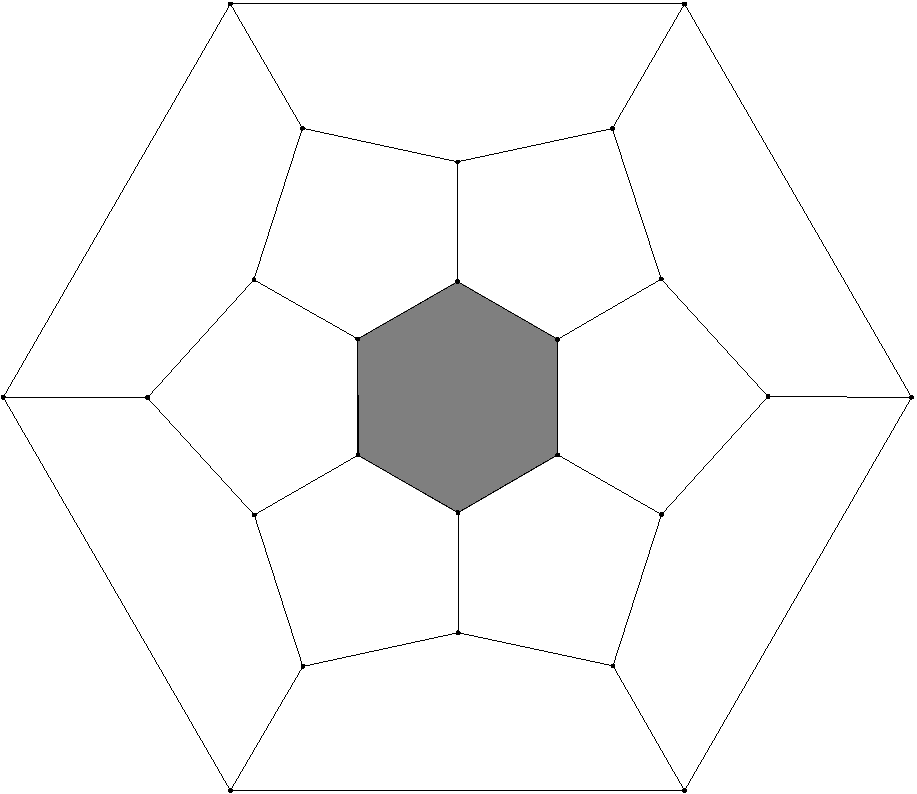
\includegraphics[bb=1 1 440 381, clip]{PictureAppli/F2sec.pdf}}\par
%24
%\end{minipage}
%\begin{minipage}[b]{2.3cm}
%\centering
%\resizebox{20mm}{!}{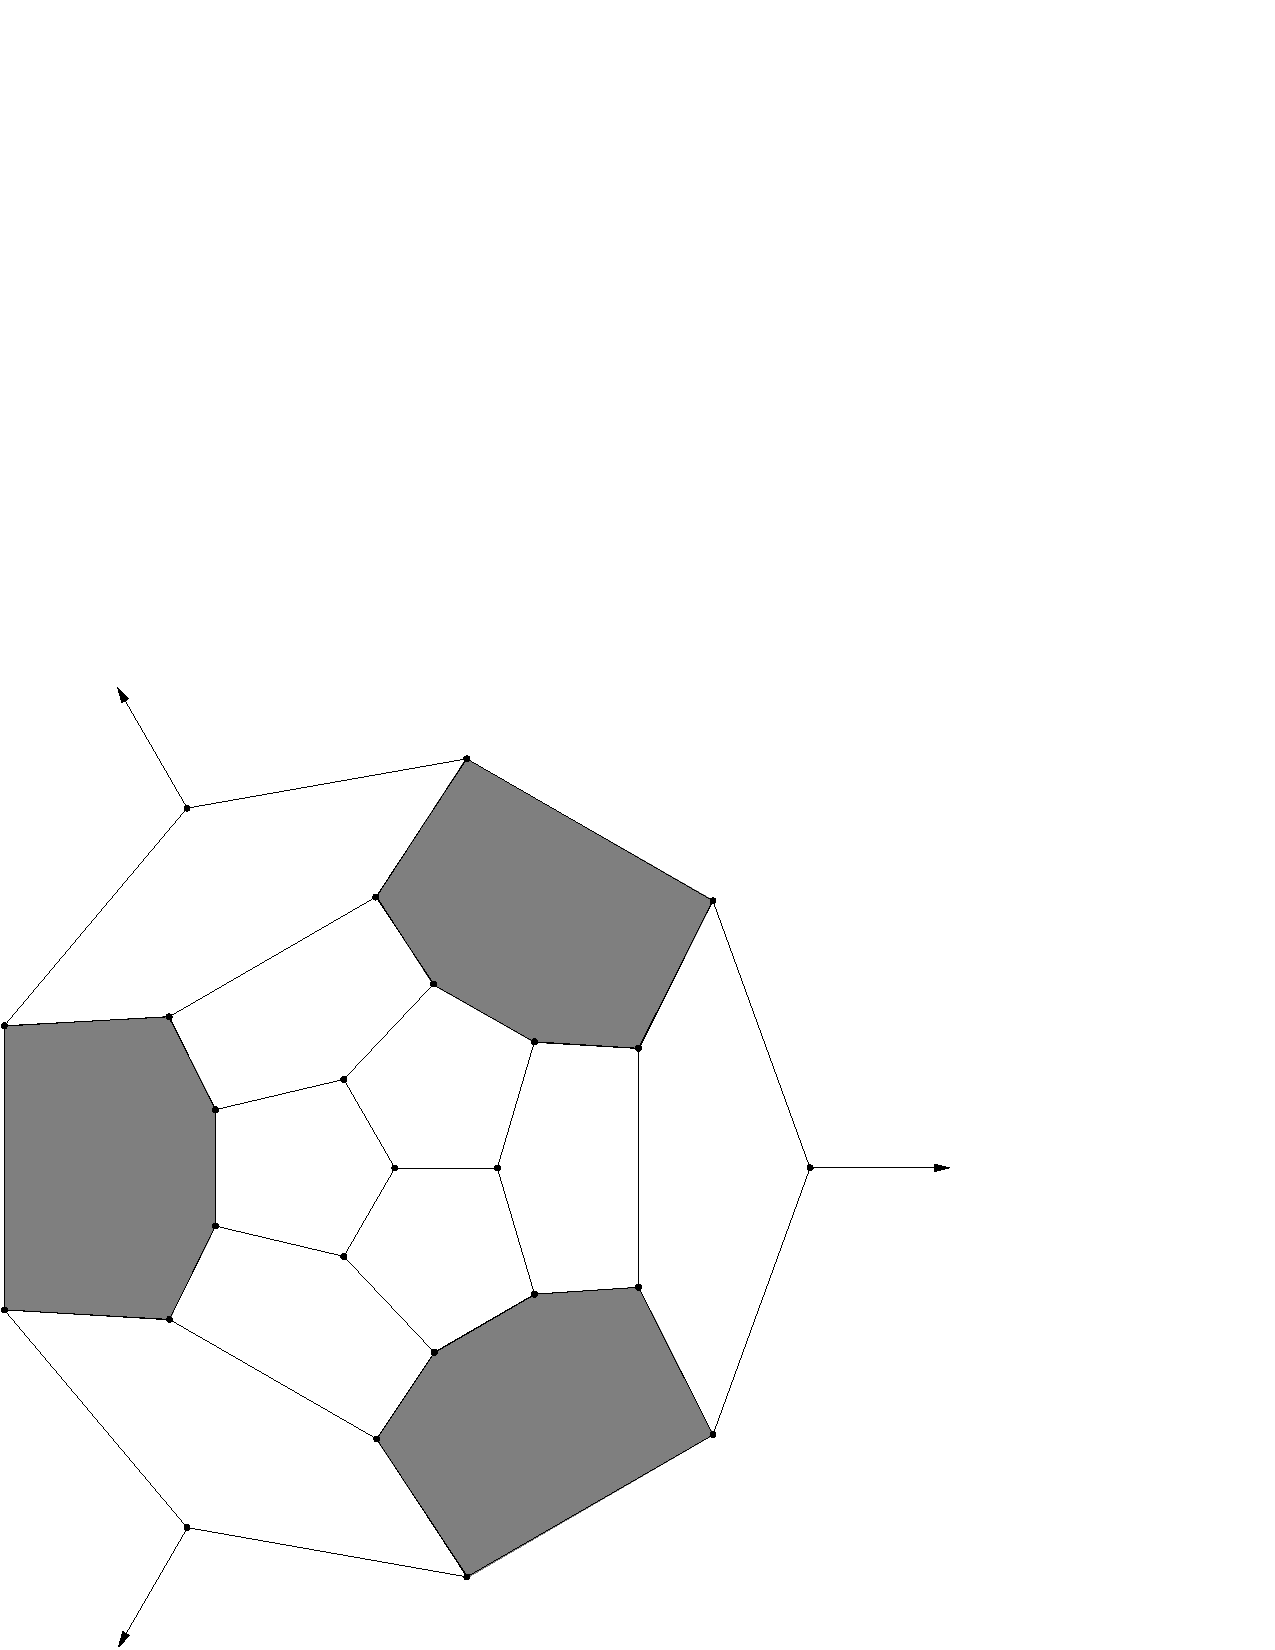
\includegraphics[bb=1 1 457 464, clip]{FullPresPic/Picture2.pdf}}\par
%26
%\end{minipage}
\begin{minipage}[b]{2.3cm}
  \centering
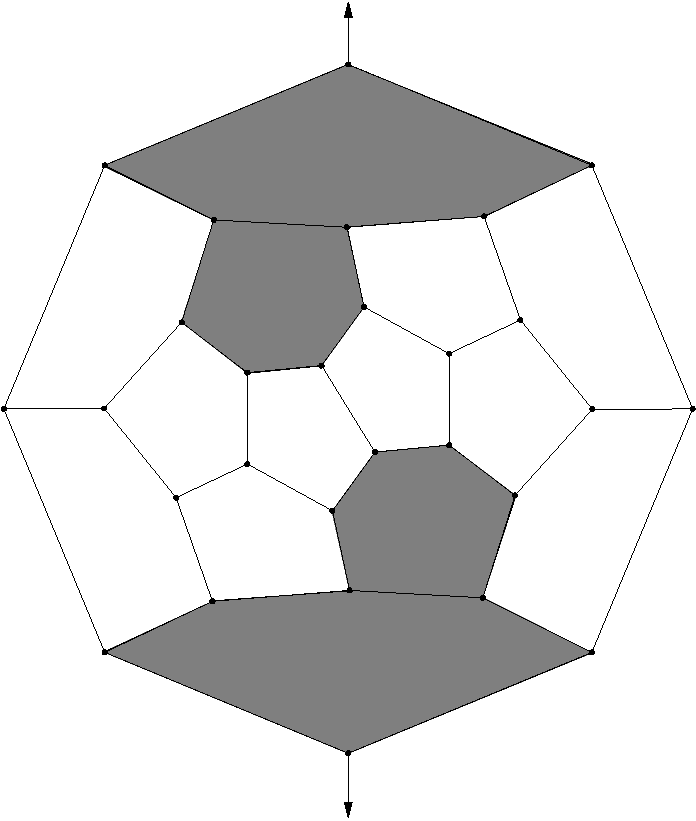
\epsfig{height=13mm, file=FullPresPic/Picture3-crop.pdf}\par
%\resizebox{13mm}{!}{\rotatebox{90}{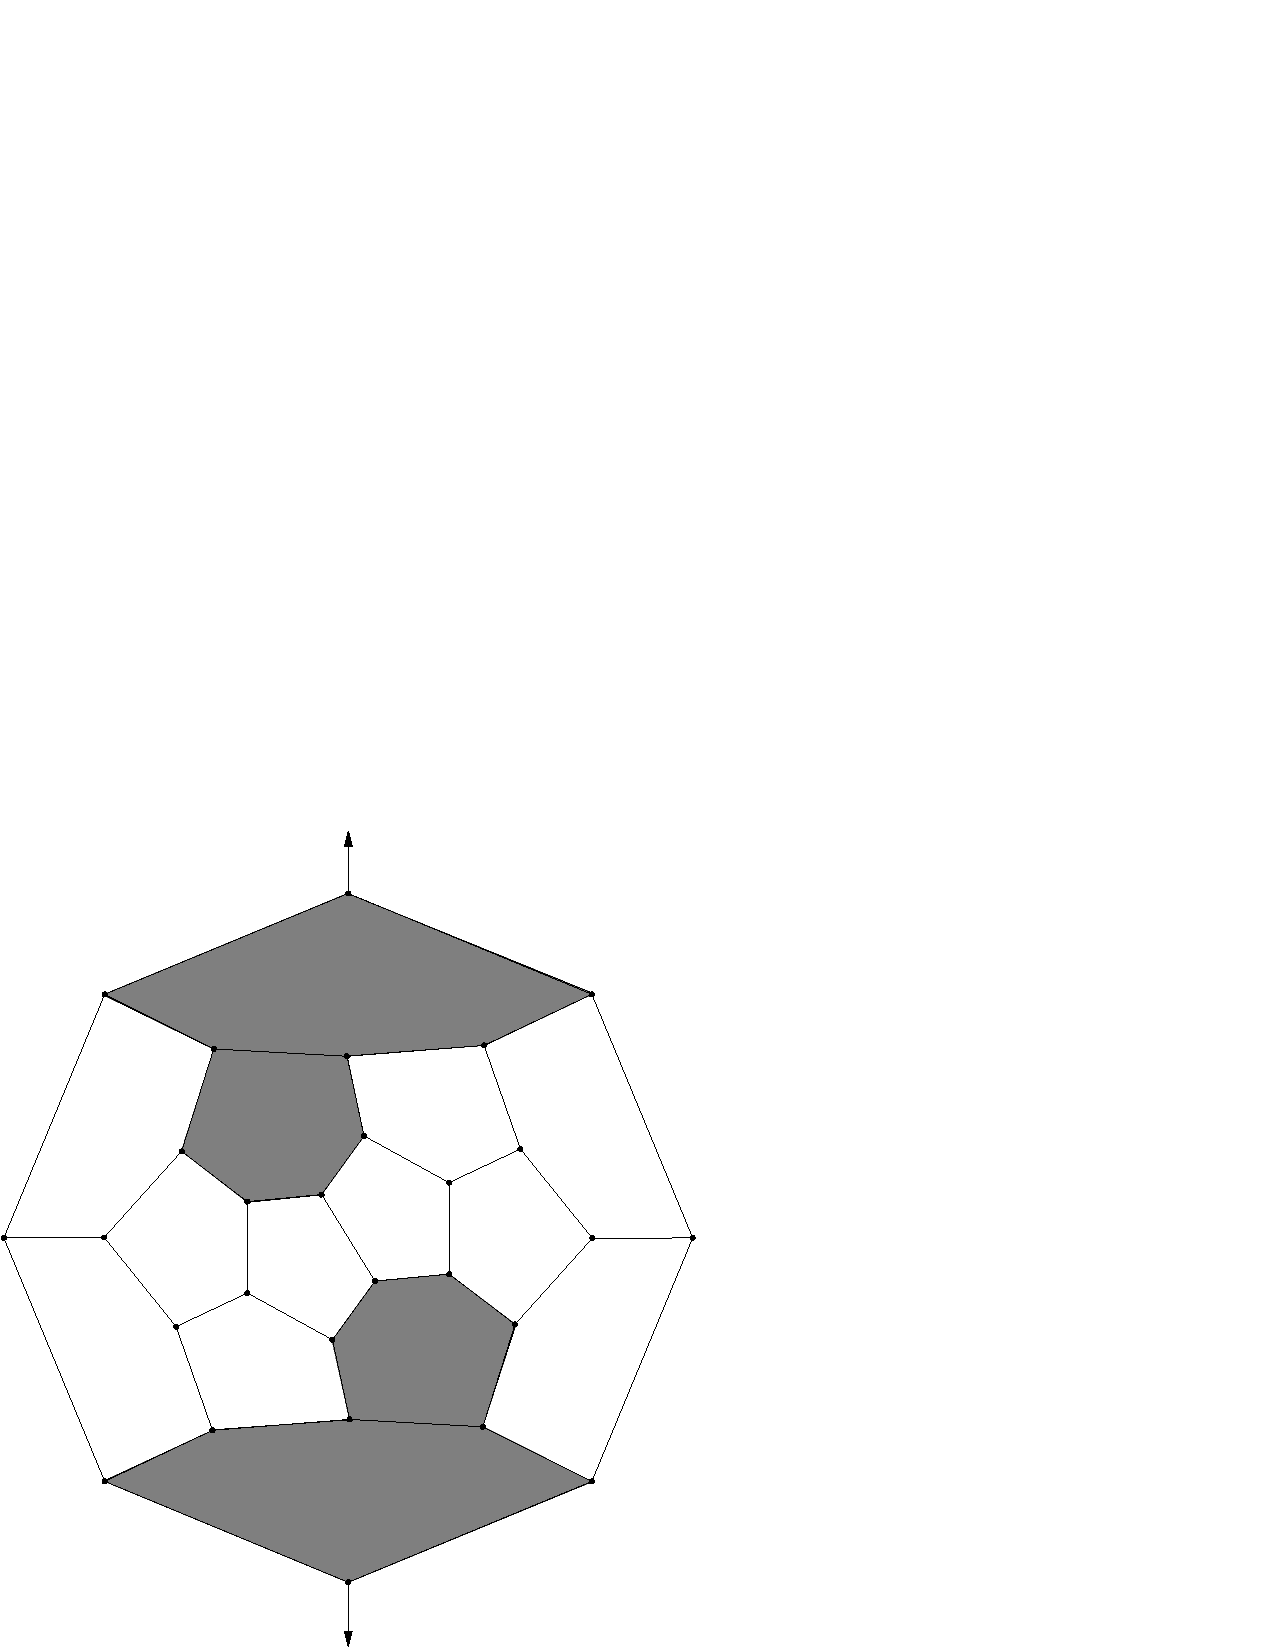
\includegraphics[bb=1 1 333 395, clip]{FullPresPic/Picture3.pdf}}}\par
\end{minipage}
%\begin{minipage}[b]{2.3cm}
%\centering
%\resizebox{20mm}{!}{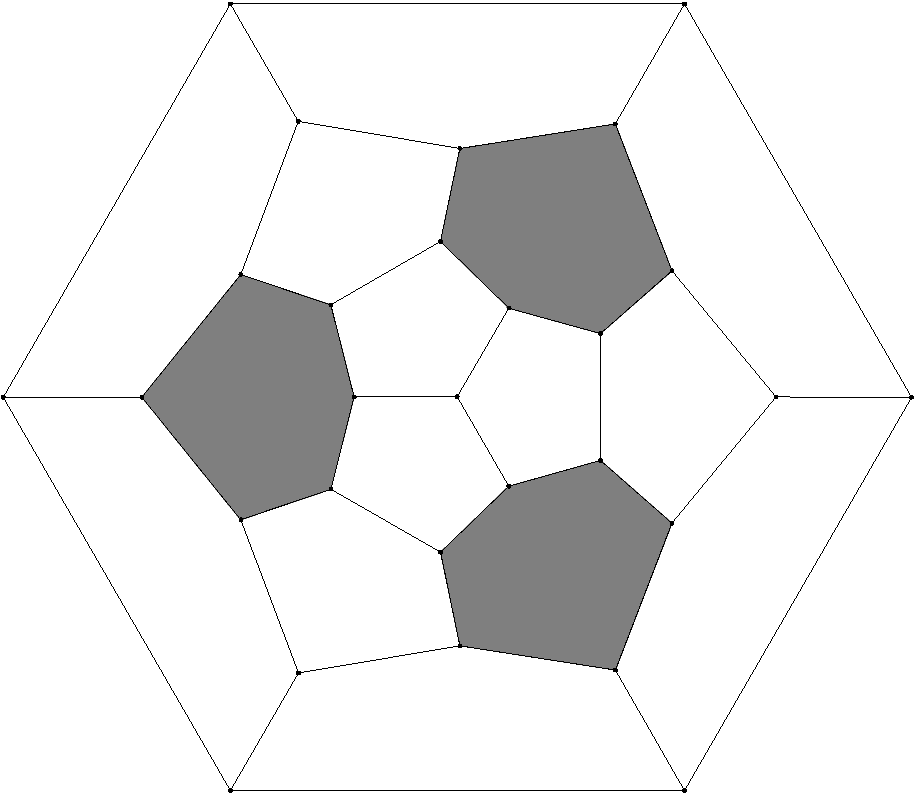
\includegraphics[bb=1 1 439 380, clip]{PictureAppli/F4sec.pdf}}\par
%28
%\end{minipage}
\begin{minipage}[b]{2.3cm}
\centering
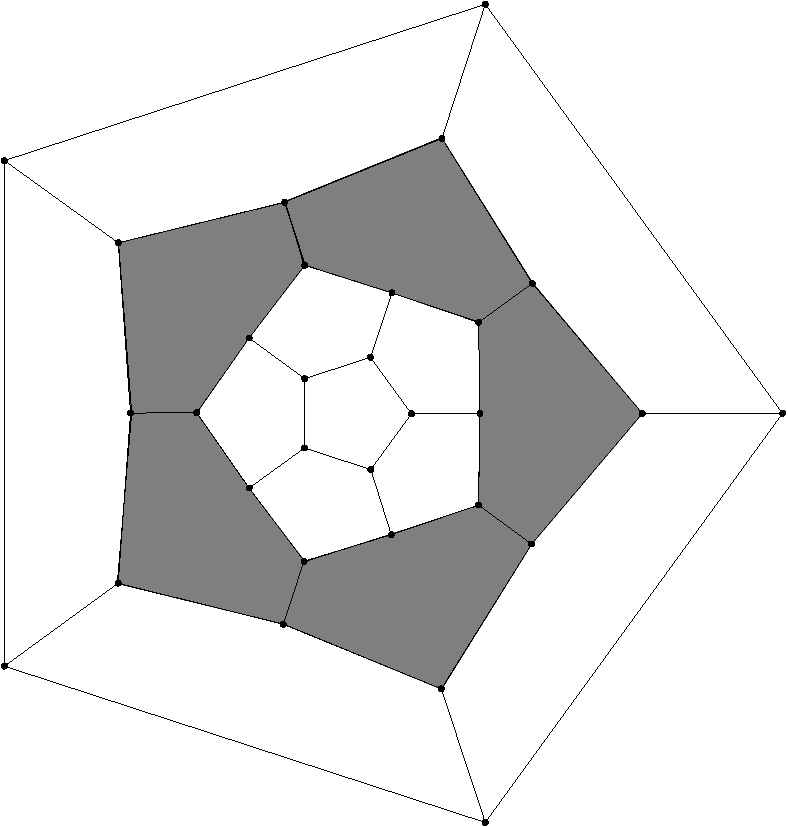
\epsfig{height=13mm, file=FullPresPic/Picture5-crop.pdf}\par
%\resizebox{11mm}{!}{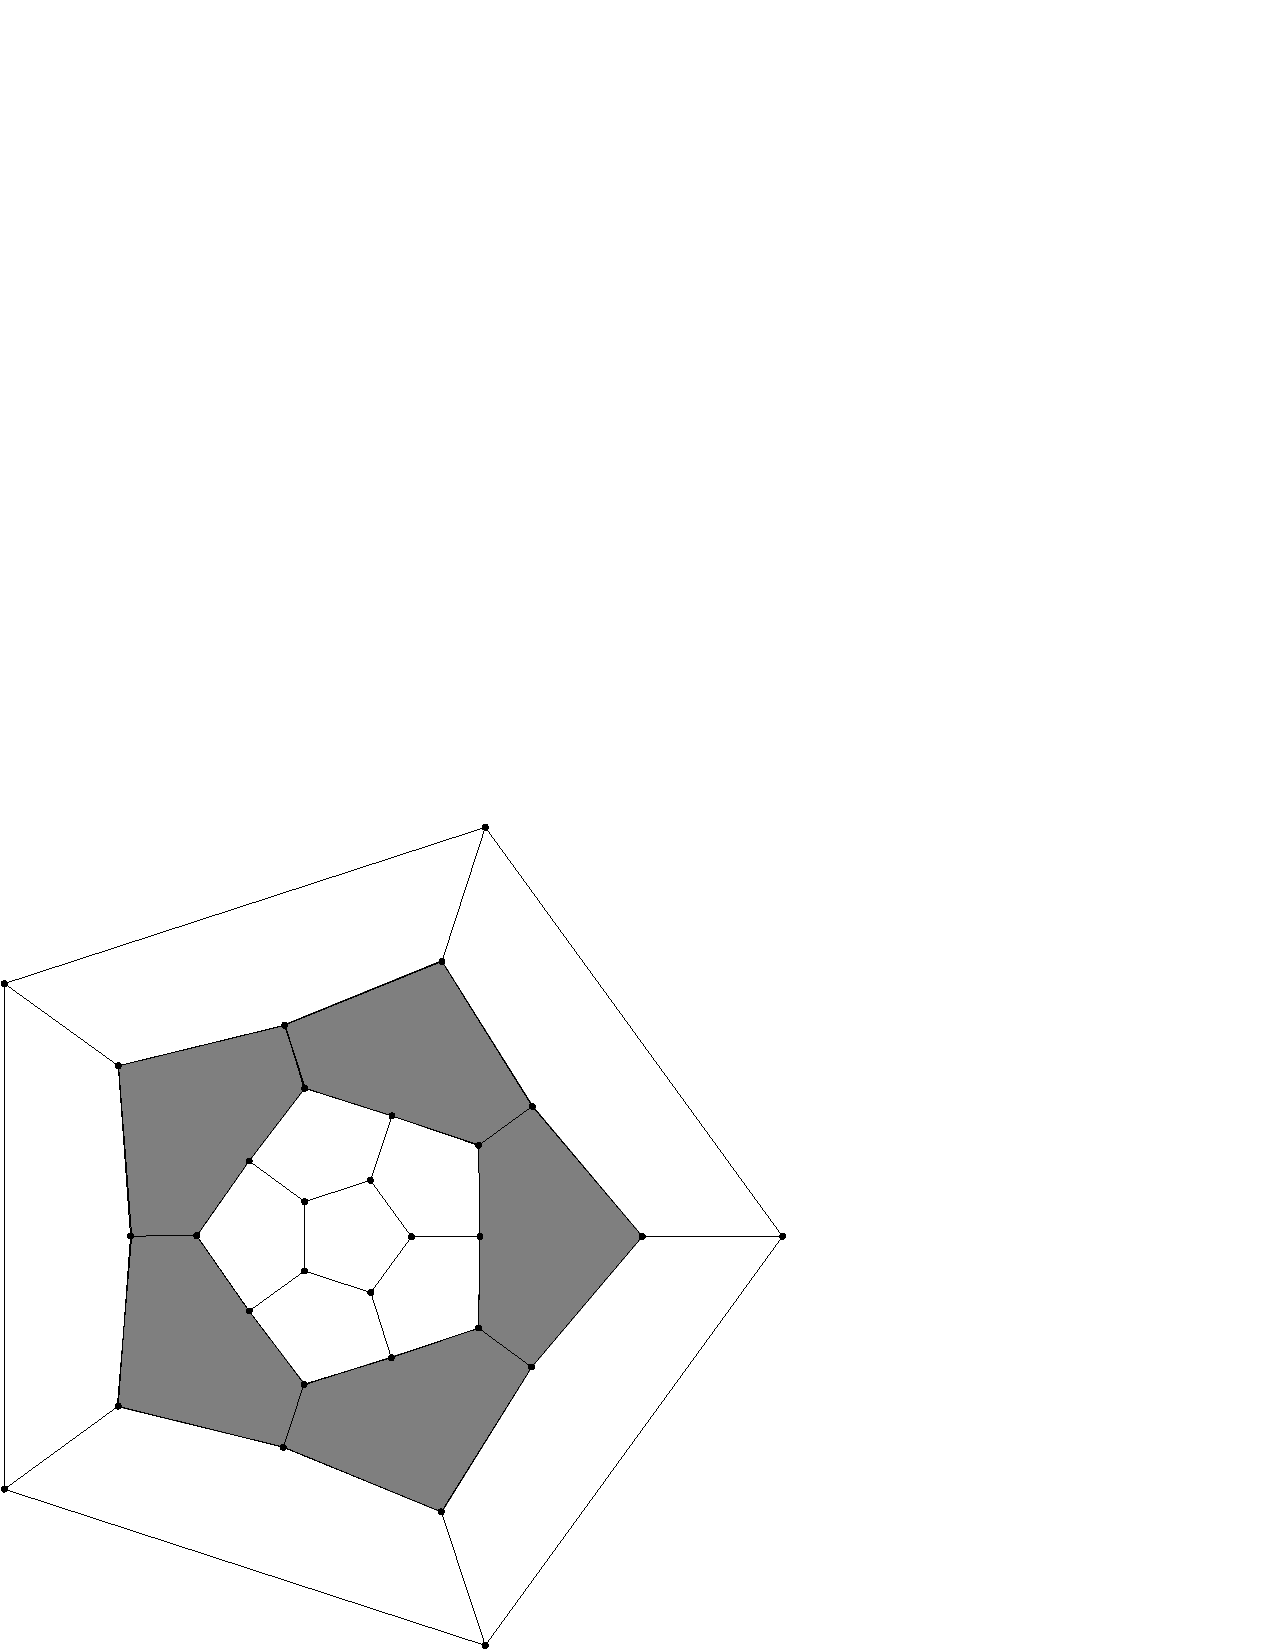
\includegraphics[bb=1 1 377 398, clip]{FullPresPic/Picture5.pdf}}\par
\end{minipage}
\begin{minipage}[b]{2.3cm}
\centering
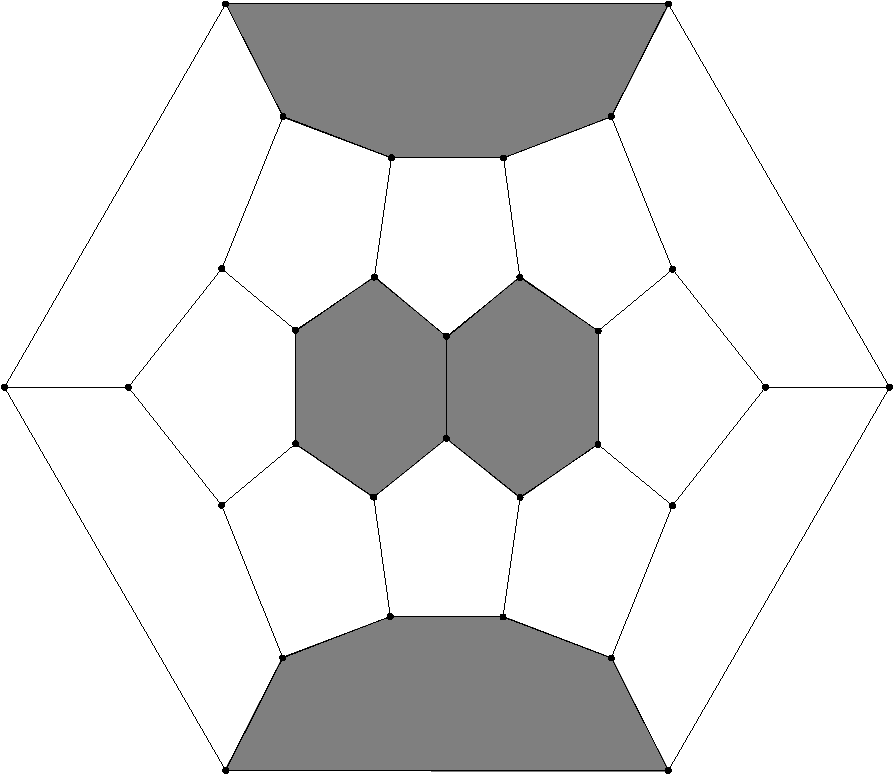
\epsfig{height=13mm, file=FullPresPic/Picture6-crop.pdf}\par
%\resizebox{13mm}{!}{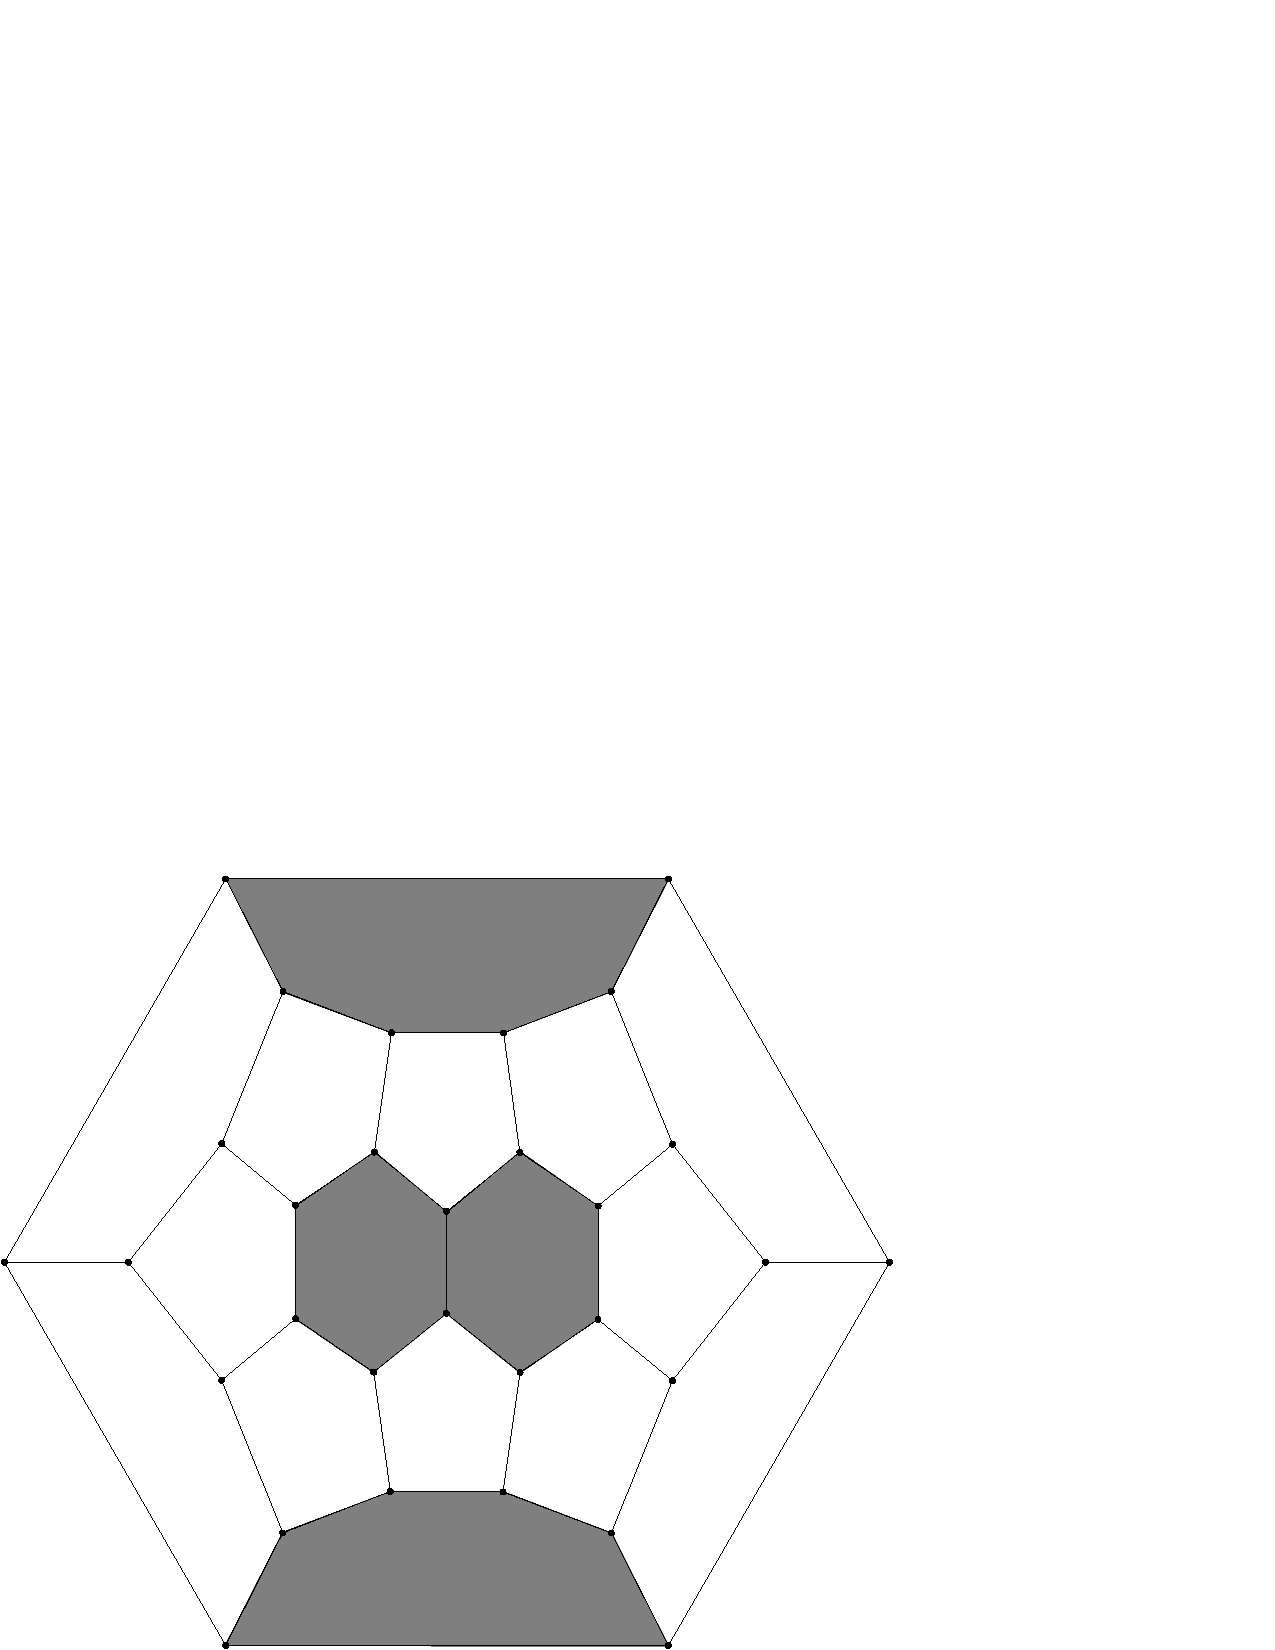
\includegraphics[bb=1 1 429 374, clip]{FullPresPic/Picture6.pdf}}\par
\end{minipage}
\begin{minipage}[b]{2.3cm}
\centering
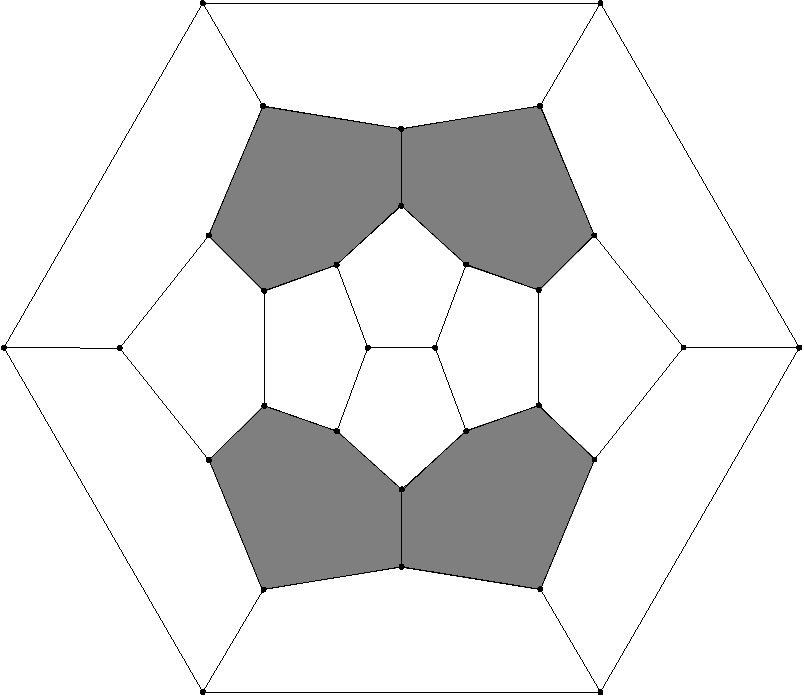
\epsfig{height=13mm, file=FullPresPic/Picture7-crop.pdf}\par
%\resizebox{13mm}{!}{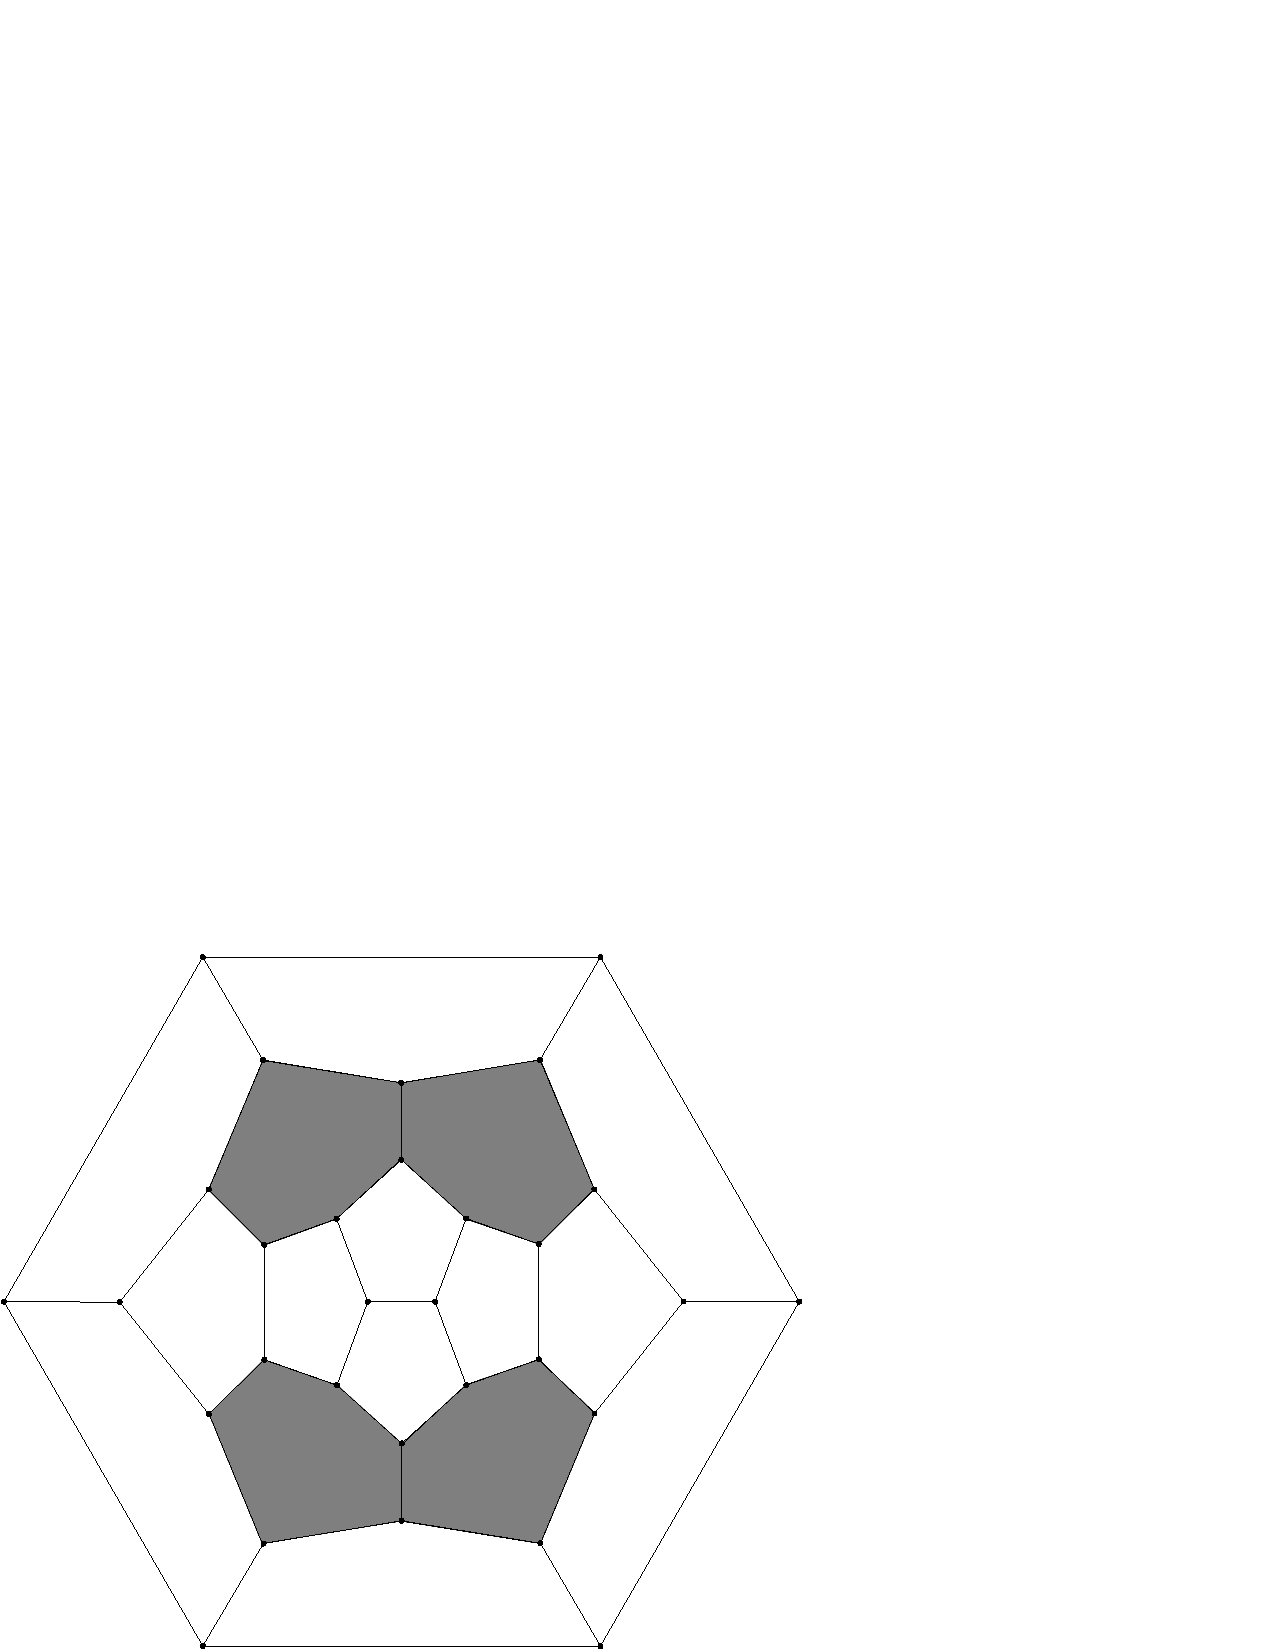
\includegraphics[bb=1 1 385 335, clip]{FullPresPic/Picture7.pdf}}\par
\end{minipage}
\end{center}
\item There exist extremely efficient programs to enumerate them (\textcolor{red}{FullGen} by G. Brinkman, \textcolor{red}{CPF} by T. Harmuth)
\item Fullerenes with isolated pentagons have $n\geq 60$. The smallest one:
\begin{center}
\begin{minipage}{4.5cm}
\centering
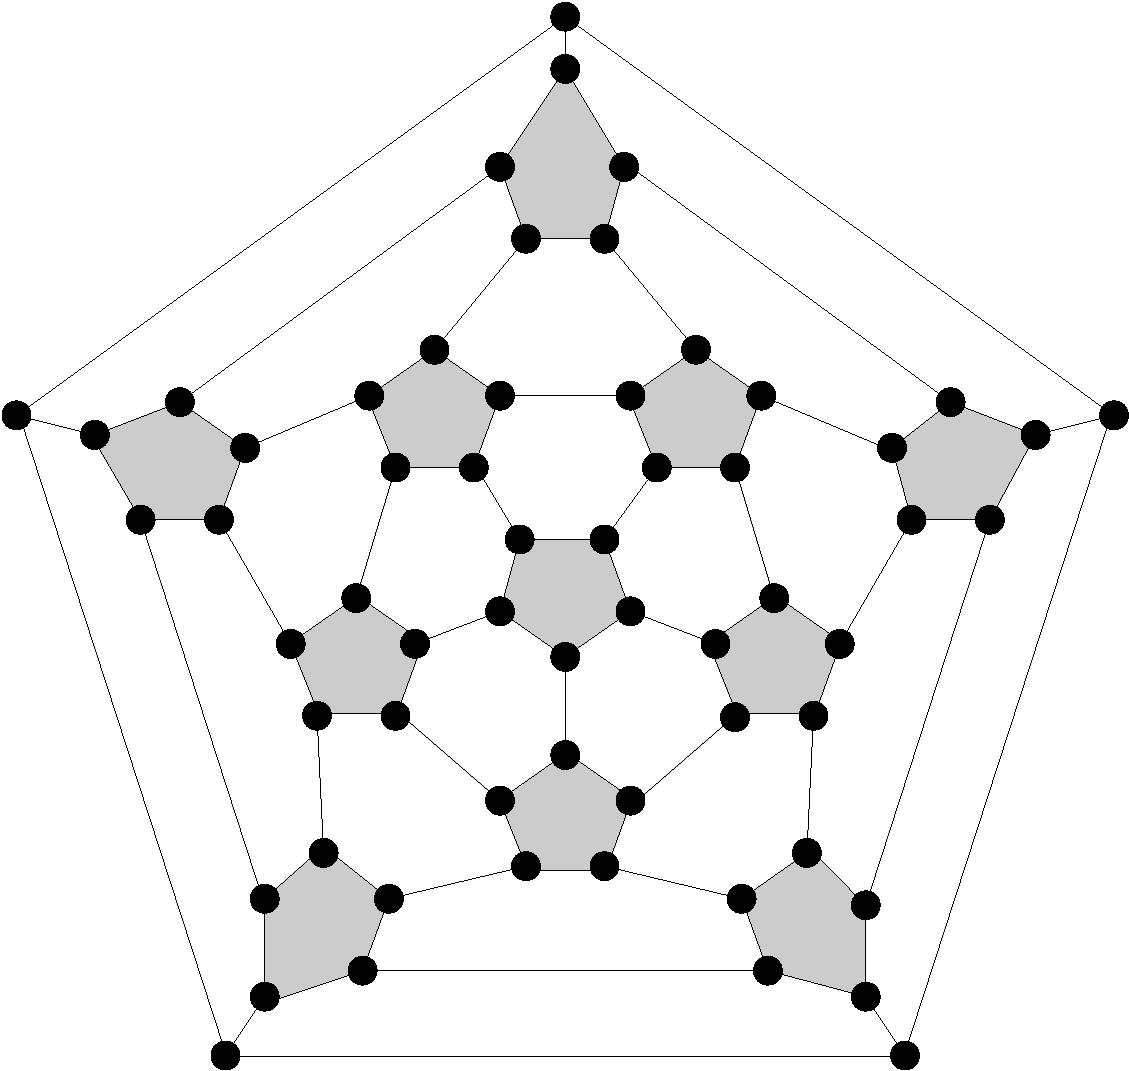
\epsfig{height=30mm, file=DRAW/PS/C60-crop.pdf}\par
%\resizebox{30mm}{!}{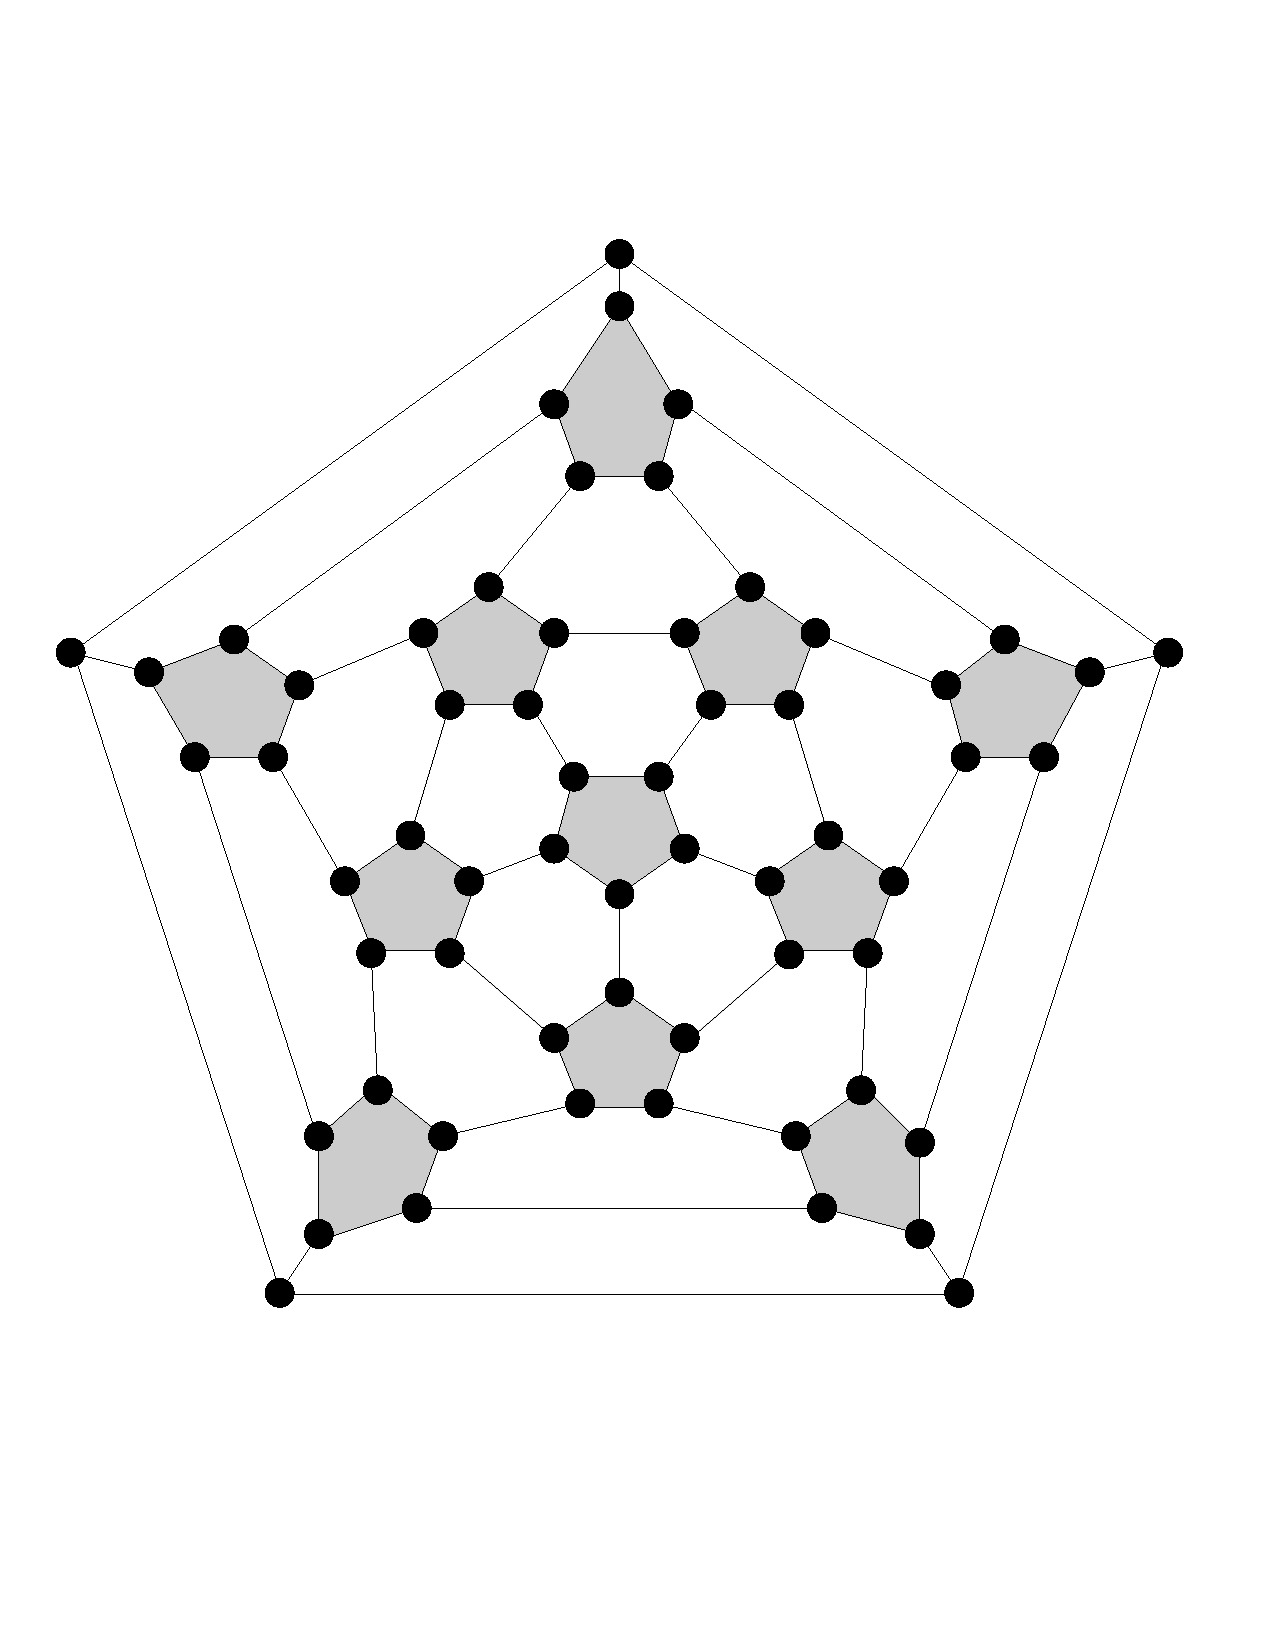
\includegraphics[bb=26 165 568 678, clip]{DRAW/PS/C60.pdf}}\par
\end{minipage}
\begin{minipage}{4.5cm}
\centering
{\em Truncated icosahedron},\par
{\em soccer ball},\par
{\em Buckminsterfullerene}
\end{minipage}


\end{center}
\end{itemize}
}






\frame{
  \frametitle{Frank Kasper structures}

\begin{itemize}
\item There are exactly $4$ fullerenes with isolated hexagons:
\begin{center}
\begin{minipage}[b]{24mm}
\centering
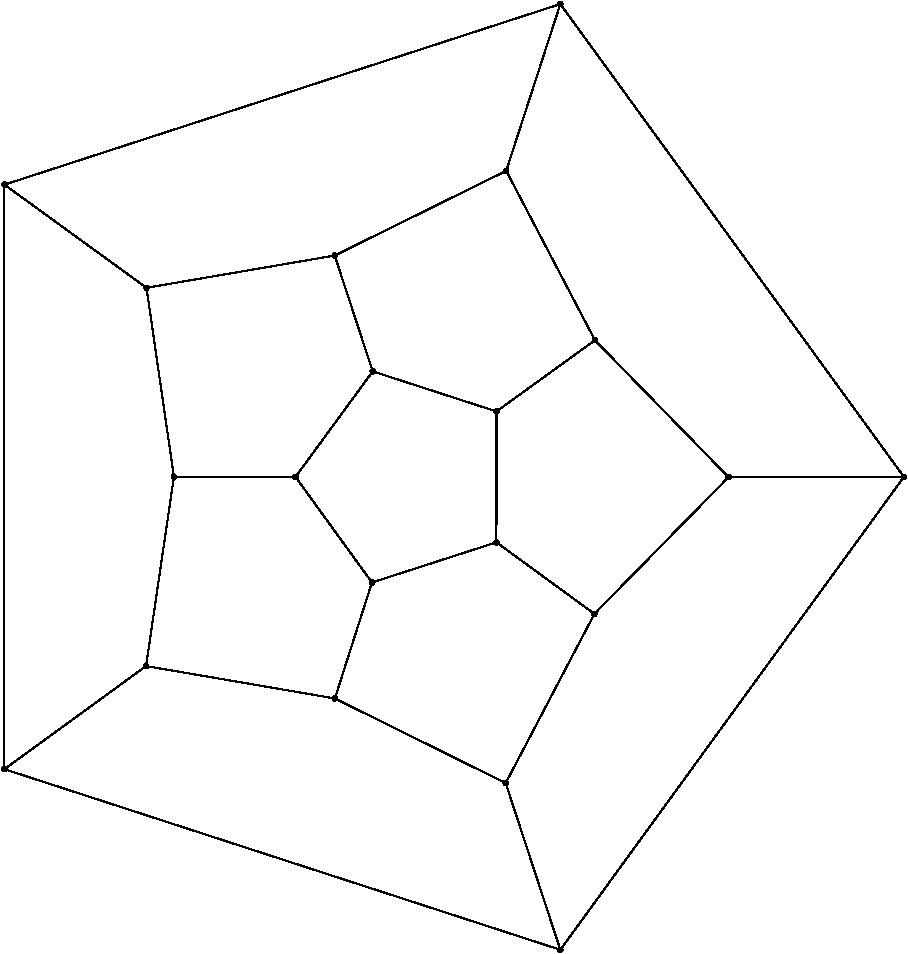
\epsfig{height=18mm, file=SpaceFullPicture/F1-crop.pdf}\par
%\resizebox{18mm}{!}{\rotatebox{90}{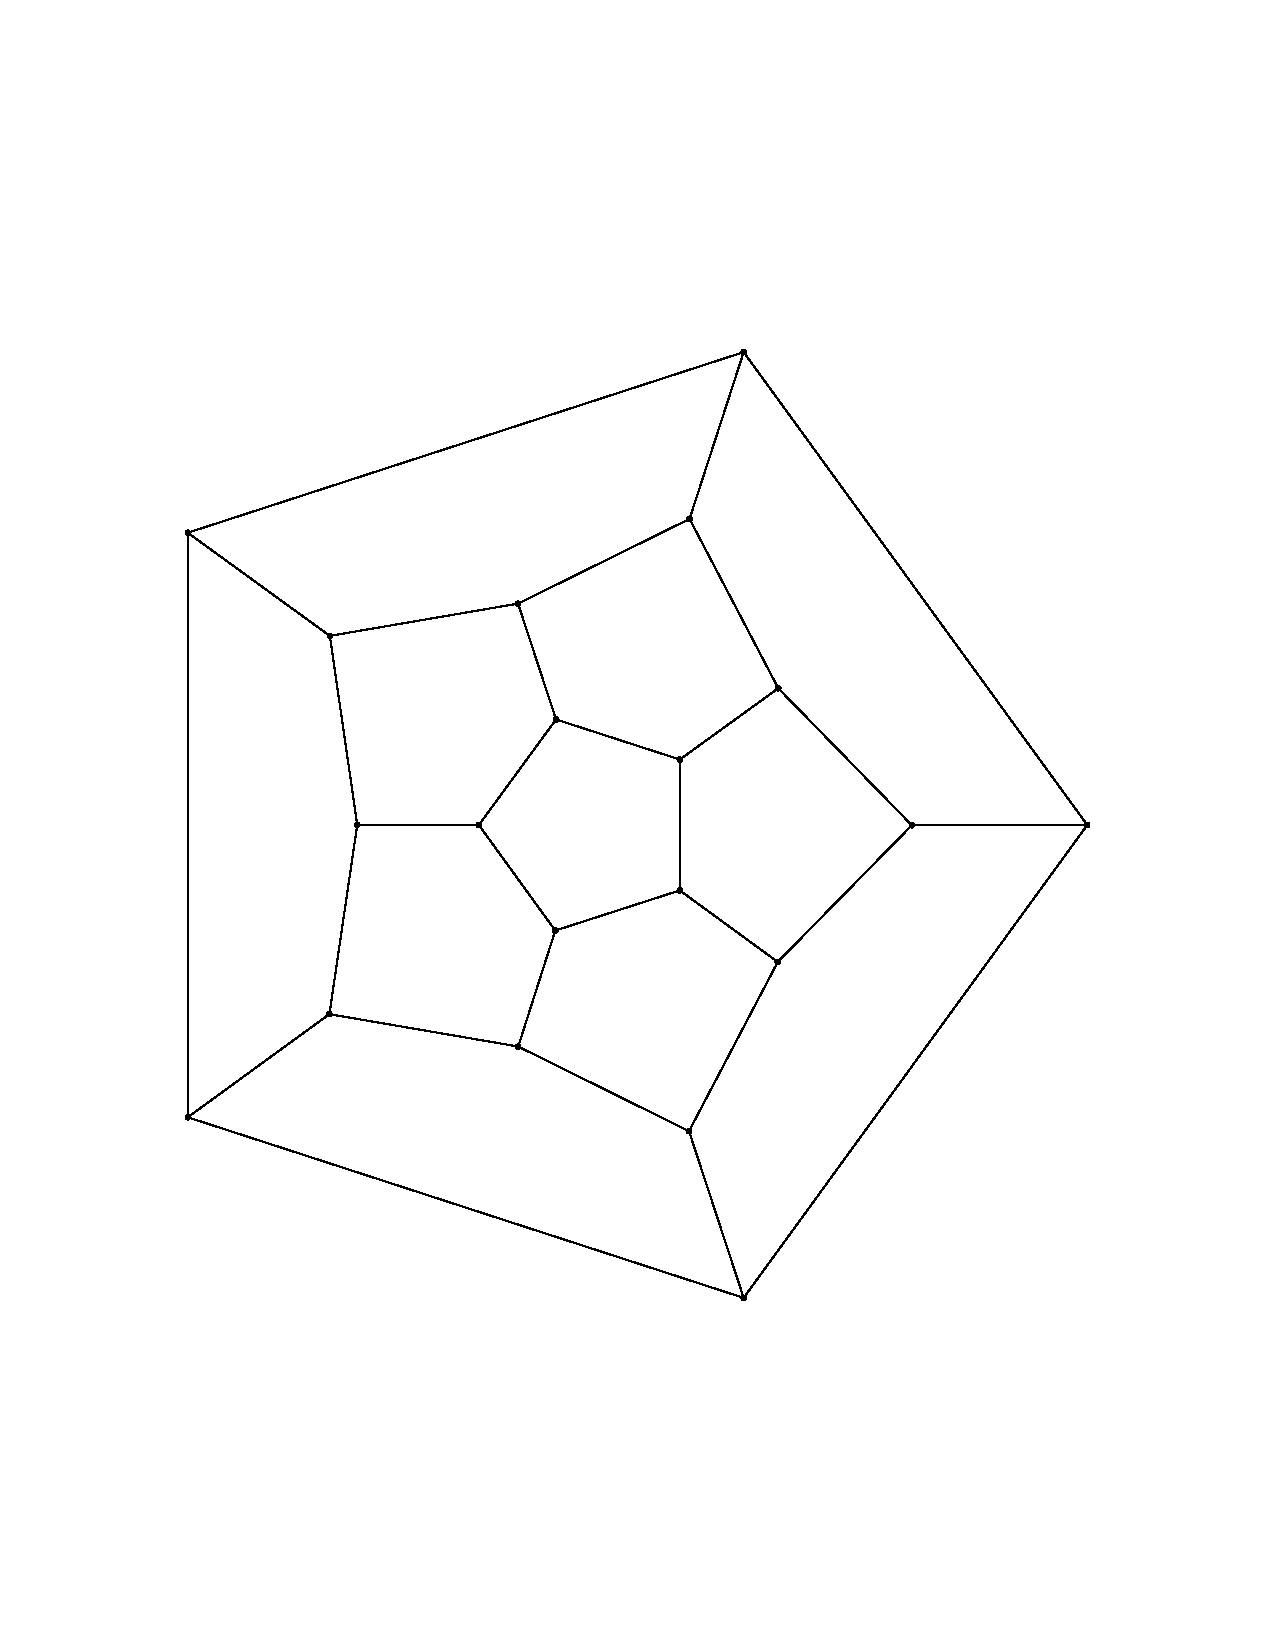
\includegraphics[bb=86 165 524 626,clip]{SpaceFullPicture/F1.pdf}}}\par
20, $I_h$
\end{minipage}
\begin{minipage}[b]{24mm}
\centering
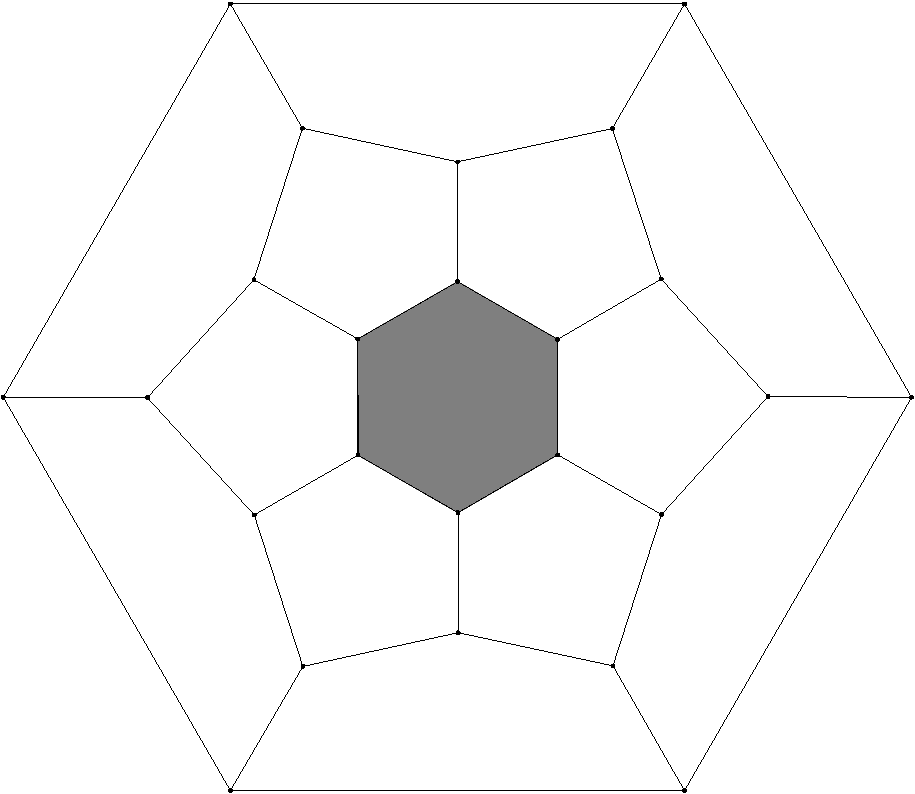
\epsfig{height=18mm, file=PictureAppli/F2sec-crop.pdf}\par
%\resizebox{20mm}{!}{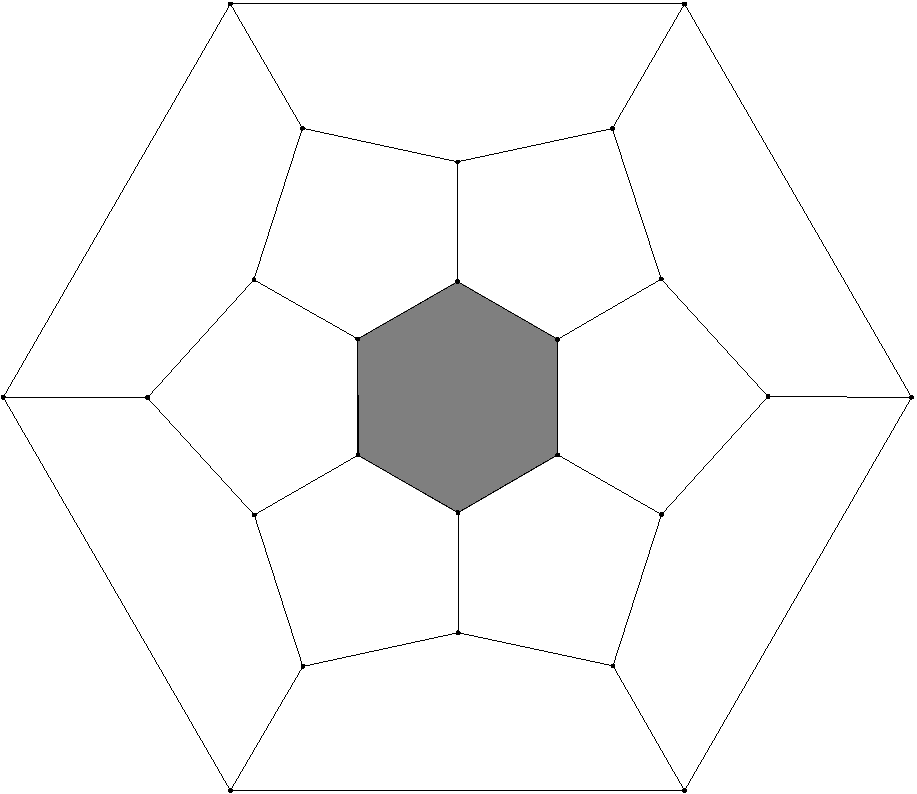
\includegraphics[bb=1 1 440 381, clip]{PictureAppli/F2sec.pdf}}\par
%\resizebox{18mm}{!}{\rotatebox{0}{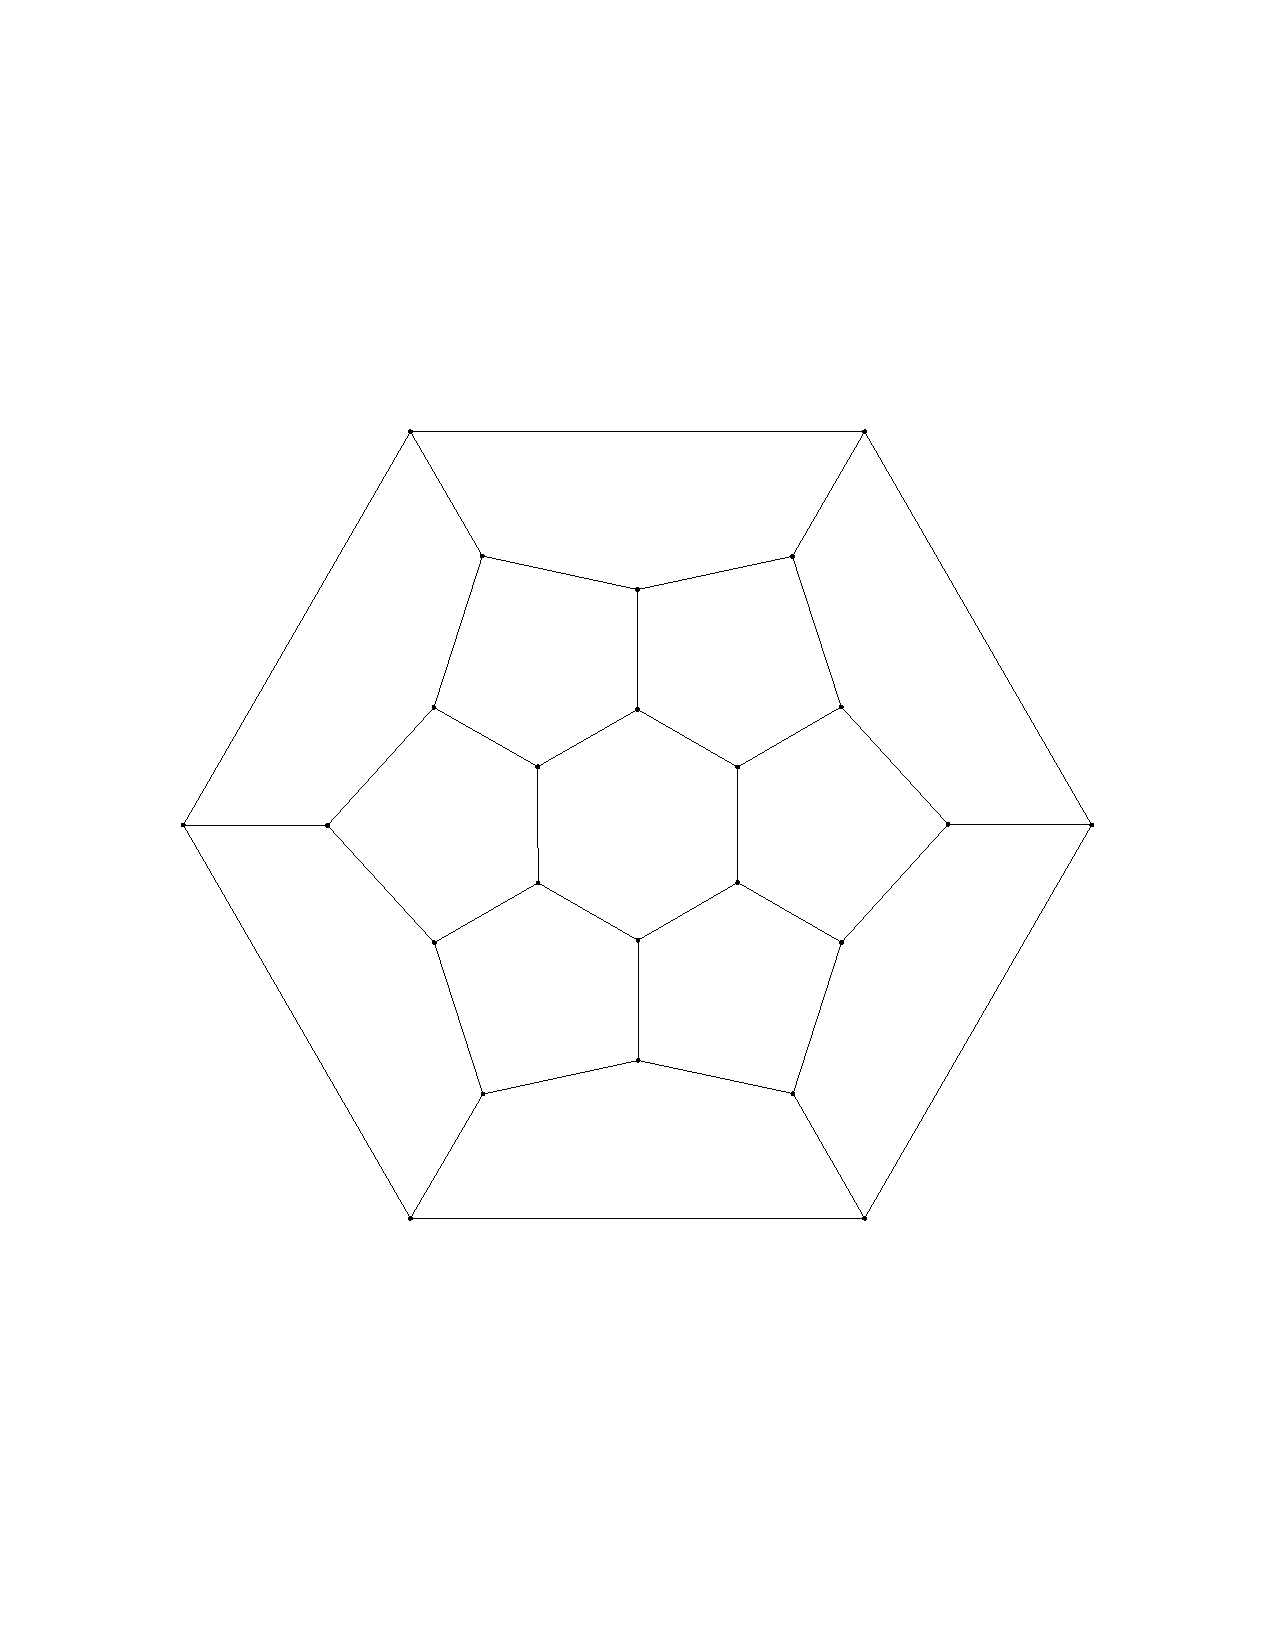
\includegraphics[bb=86 206 524 590,clip]{SpaceFullPicture/F2.pdf}}}\par
24 $D_{6d}$
\end{minipage}
\begin{minipage}[b]{24mm}
  \centering
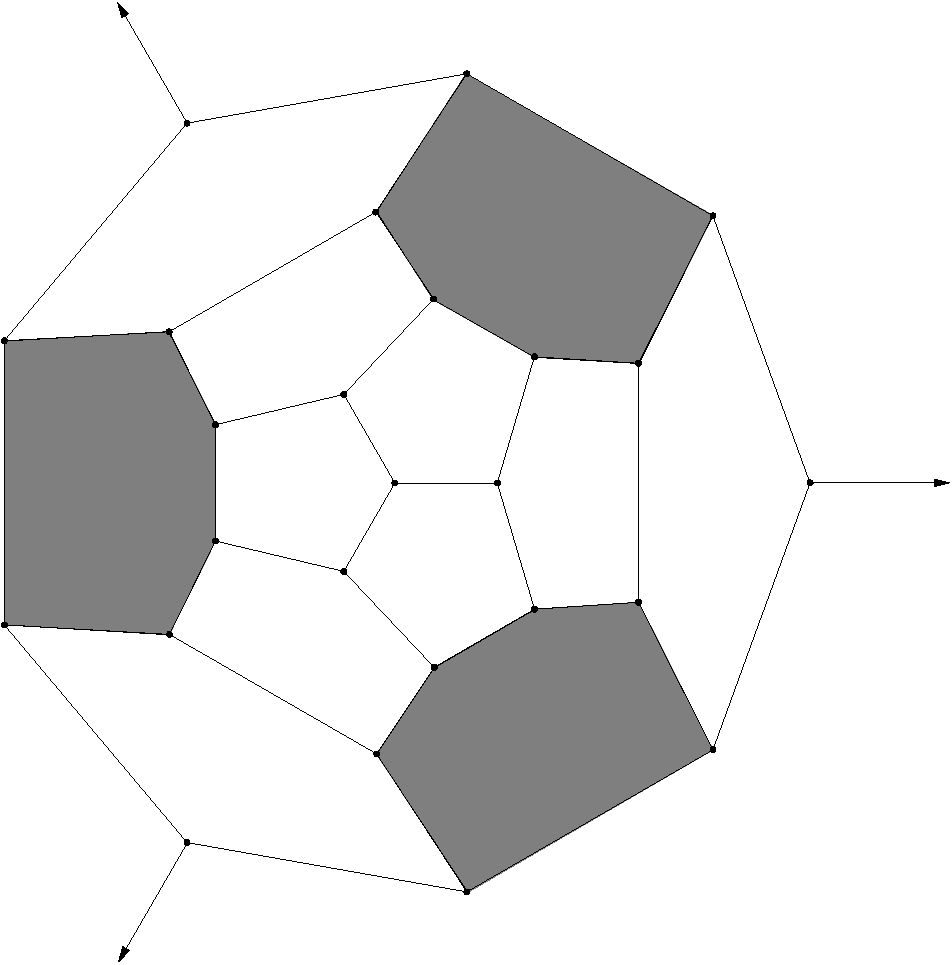
\epsfig{height=18mm, file=FullPresPic/Picture2-crop.pdf}\par
%\resizebox{20mm}{!}{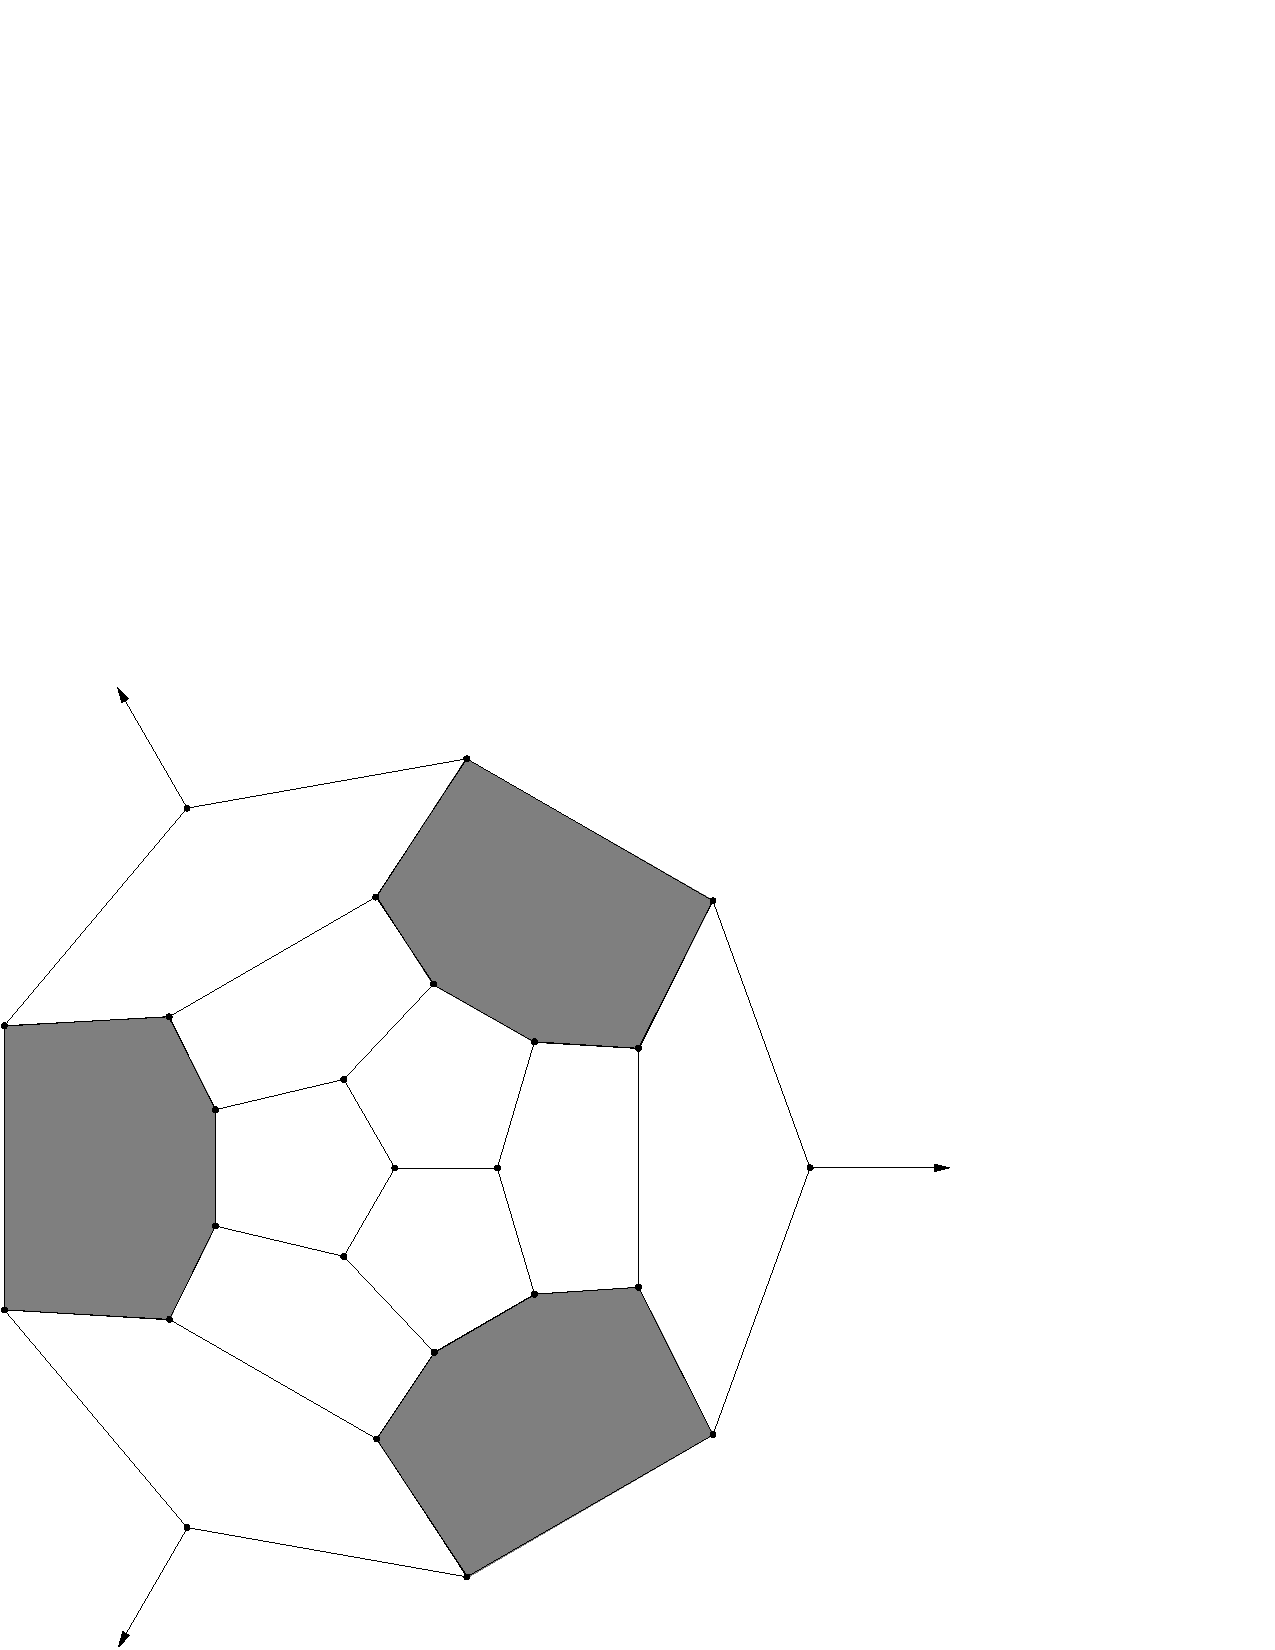
\includegraphics[bb=1 1 457 464, clip]{FullPresPic/Picture2.pdf}}\par
%\resizebox{18mm}{!}{\rotatebox{0}{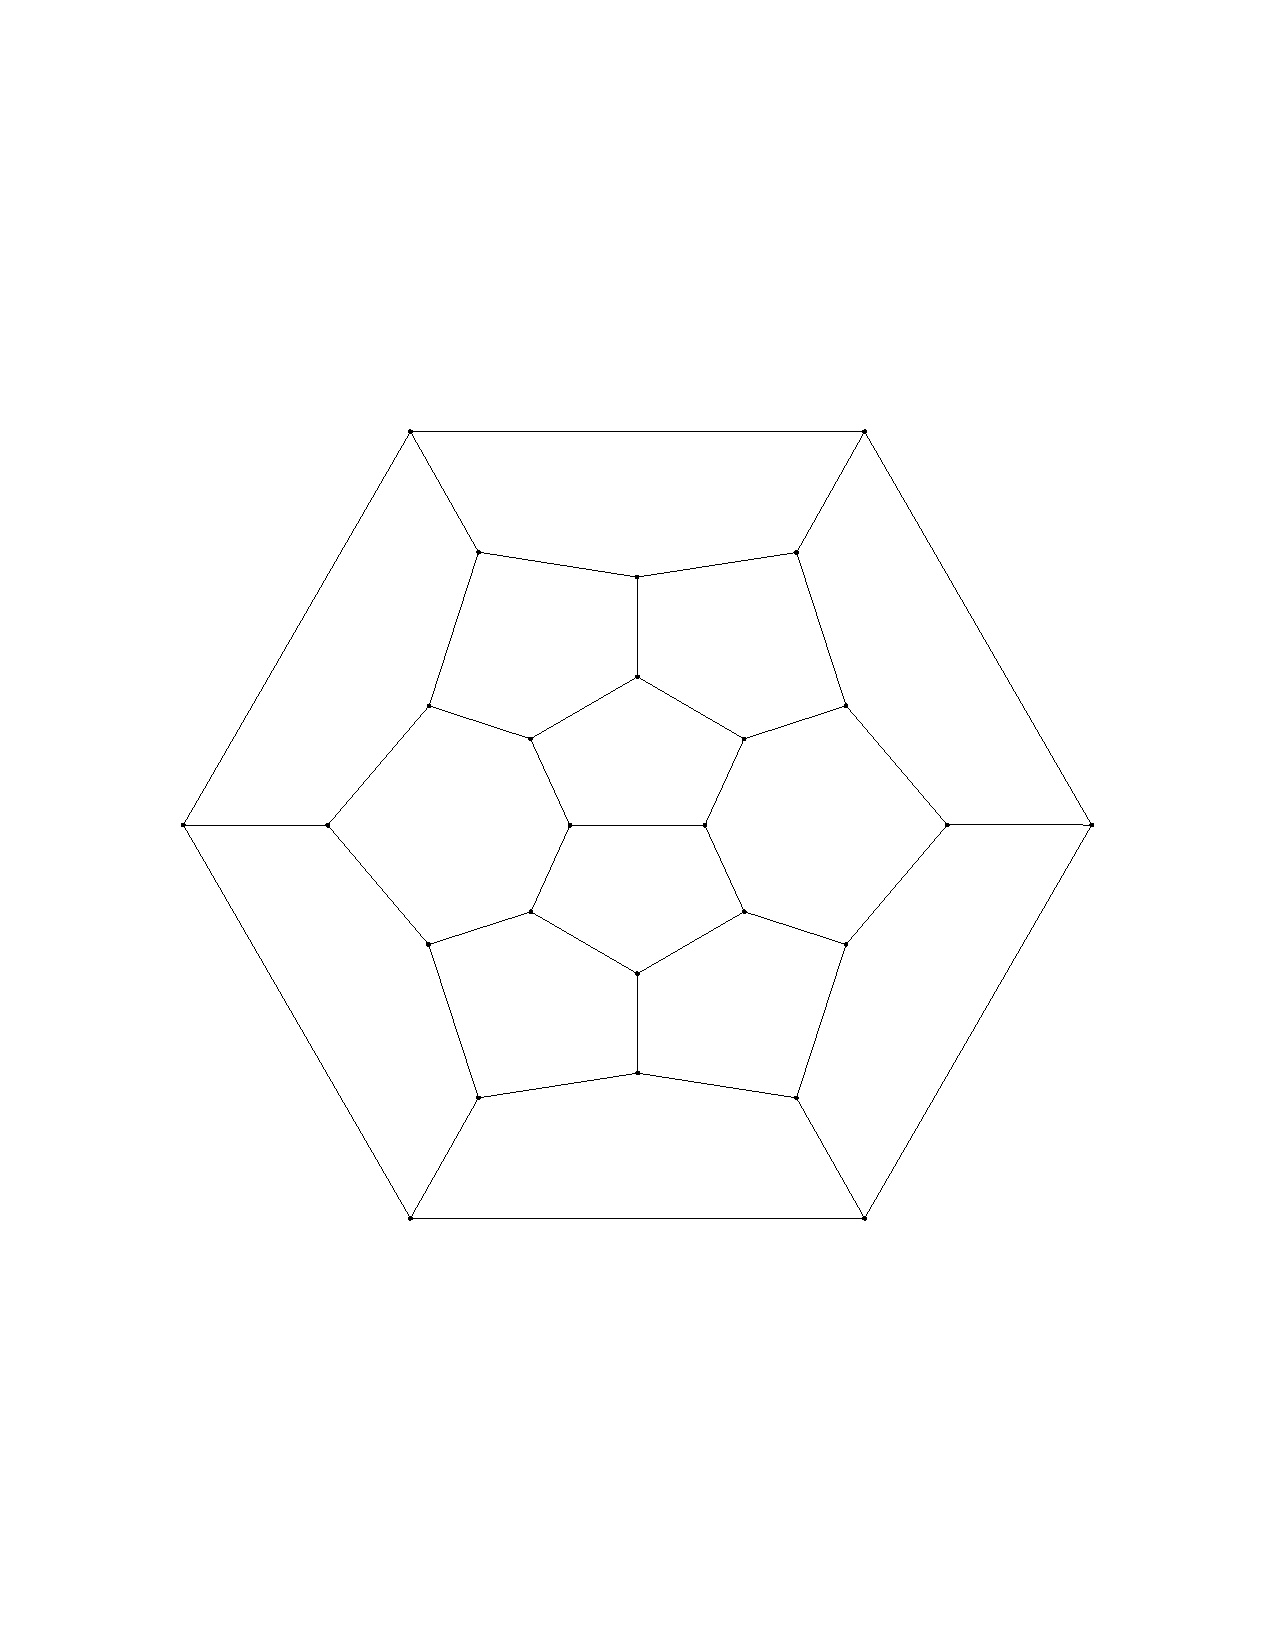
\includegraphics[bb=86 206 524 590,clip]{SpaceFullPicture/F3.pdf}}}\par
26, $D_{3h}$
\end{minipage}
\begin{minipage}[b]{24mm}
  \centering
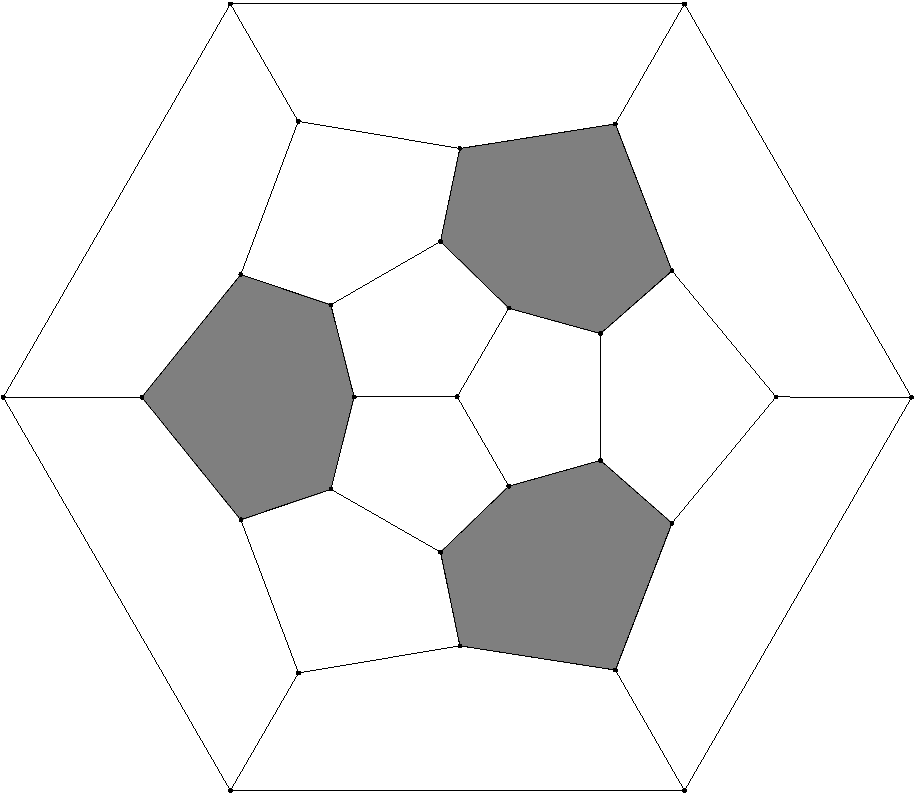
\epsfig{height=18mm, file=PictureAppli/F4sec-crop.pdf}\par
%\resizebox{20mm}{!}{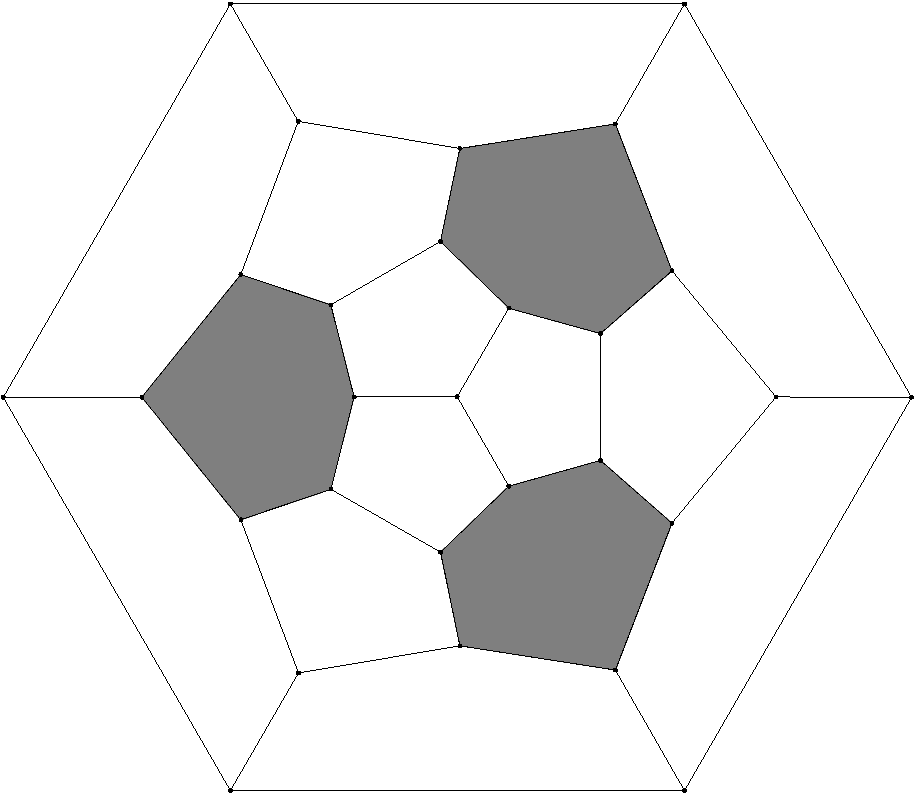
\includegraphics[bb=1 1 439 380, clip]{PictureAppli/F4sec.pdf}}\par
%\resizebox{18mm}{!}{\rotatebox{0}{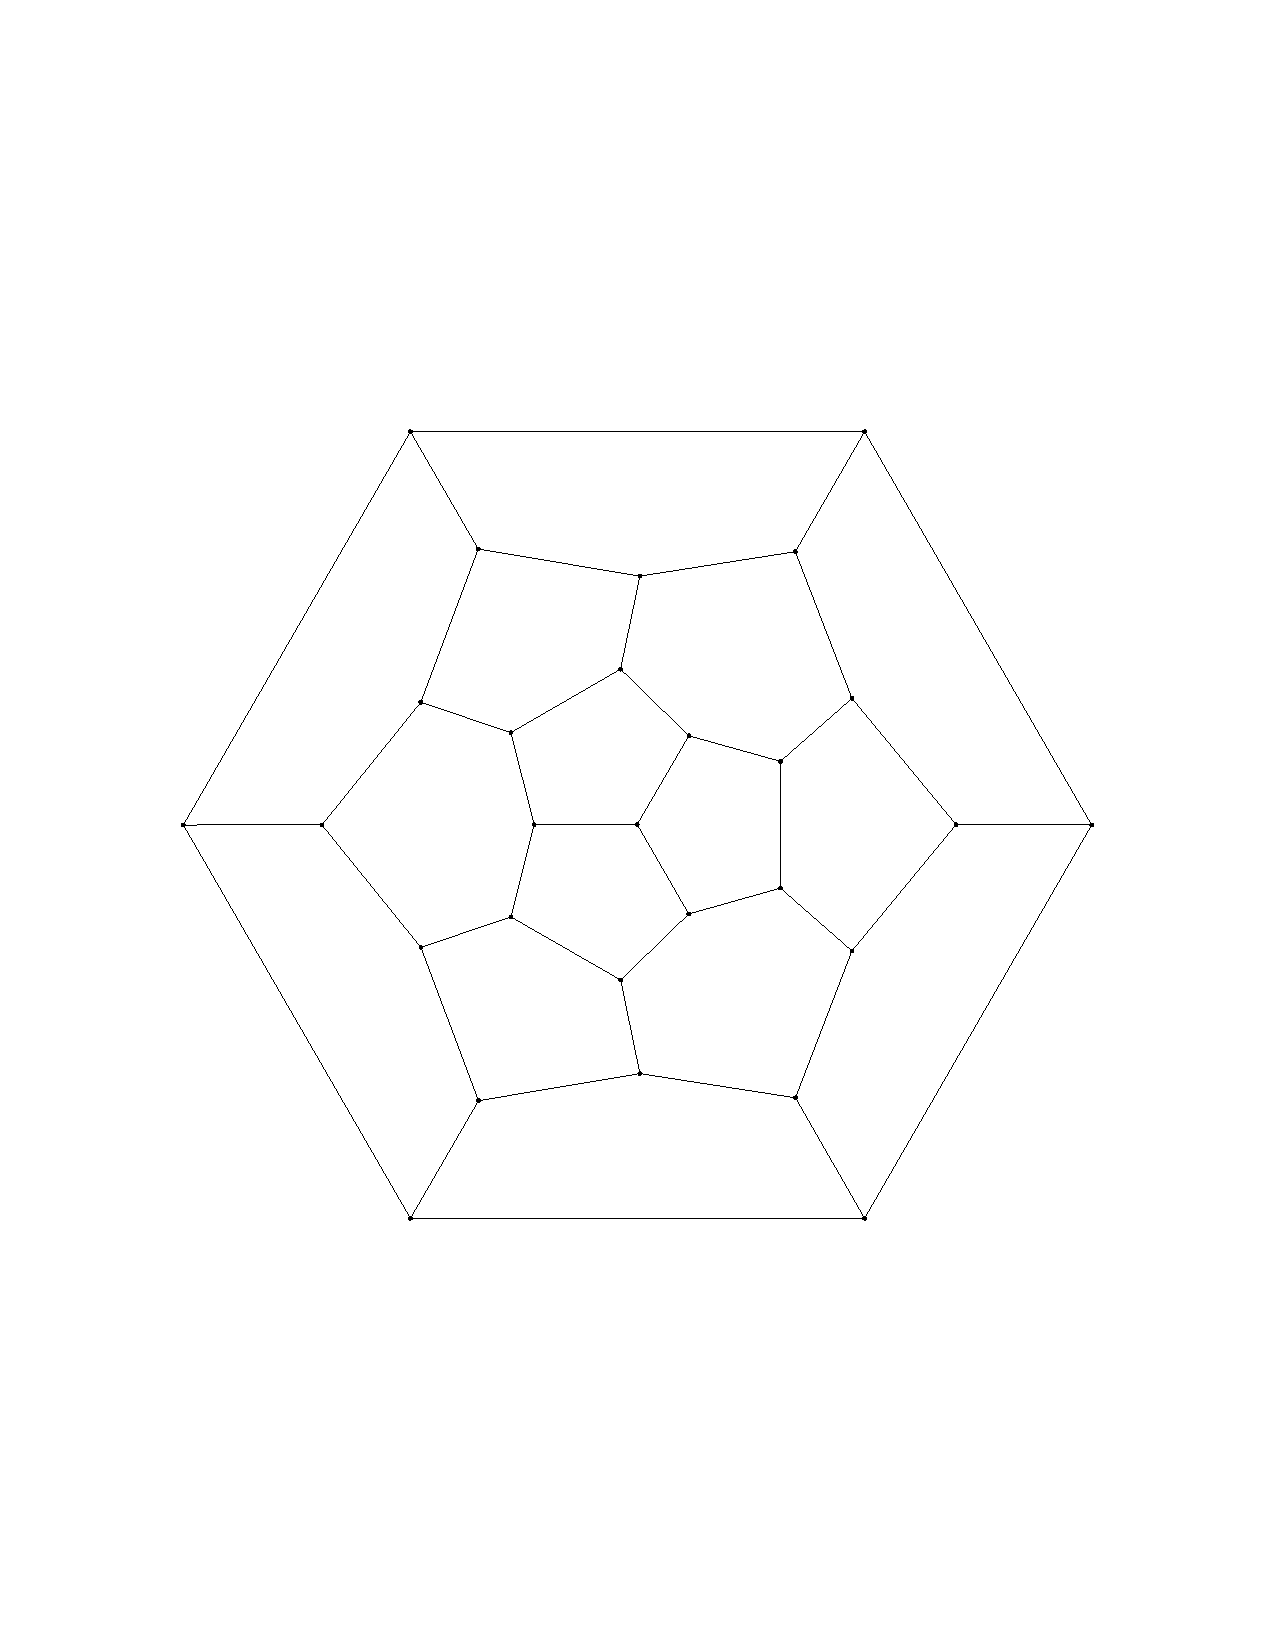
\includegraphics[bb=86 206 524 590,clip]{SpaceFullPicture/F4.pdf}}}\par
28, $T_{d}$
\end{minipage}
\end{center}
\item A \textcolor{red}{Space-fullerene} structure is a $4$-valent $3$-periodic tiling of $\RR^3$ by those $4$ fullerenes.
\item They were introduced by Frank \& Kasper in two papers in 1958, 1959 in order to explain a variety of crystallographic structures in a unified way.
\item The basic problems are:
\begin{itemize}
\item Find the possible structures, they are very rare.
\item Find some general constructions.
\item Find structural properties.
\end{itemize}

\end{itemize}
}


\frame{
  \frametitle{Known Physical phases I}

\begin{itemize}
\item \textcolor{red}{group} is the space group according to the crystallographic tables
\item \textcolor{red}{fund. dom.} is the number of cells in a fundamental domain.
\item \textcolor{red}{fraction} $(x_{20}, x_{24}, x_{26}, x_{28})$ is the relative number of $20$-, $24$-, $26$- and $28$-cells in 
\end{itemize}
\begin{center}
{\small
\begin{tabular}{|c|c|c|c|c|}
\cline{1-5}
phase & rep. alloy & group & fund. dom. & fraction\\
\cline{1-5}
$C_{14}$ & ${\rm Mg} {\rm Zn}_{2}$ & $P6_3/mmc$ & $12$ & $(2,0,0,1)$\\
$C_{15}$ & ${\rm Mg} {\rm Cu}_{2}$ & $Fd\overline{3}m$ & $24$ & $(2,0,0,1)$\\
$C_{36}$ & ${\rm Mg} {\rm Ni}_{2}$ & $P6_3/mmc$ & $24$ &  $(2,0,0,1)$\\
$6$-layers & ${\rm Mg} {\rm Cu} {\rm Ni}$ & $P6_3/mmc$ & $36$ &  $(2,0,0,1)$\\
$8$-layers & ${\rm Mg} {\rm Zn}_2 + 0.03 {\rm Mg} {\rm Ag}_2$ & $P6_3/mmc$ & $48$ & $(2,0,0,1)$\\
$9$-layers & ${\rm Mg} {\rm Zn}_2 + 0.07 {\rm Mg} {\rm Ag}_2$ & $R\overline{3}m$ & $54$ & $(2,0,0,1)$\\
$10$-layers & ${\rm Mg} {\rm Zn}_2 + 0.1 {\rm Mg} {\rm Ag}_2$ & $P6_3/mmc$ & $60$ & $(2,0,0,1)$\\
$-$ & ${\rm Mg}_4{\rm Zn}_7$ & $C2/m$ & $110$ & $(35,2,2,16)$\\
$X$ & ${\rm Mn}_{45} {\rm Co}_{40} {\rm Si}_{15}$ & $Pnnm$ & $74$ & $(23,2,2,10)$\\
$T$ & ${\rm Mg}_{32}(Zn, Al)_{49}$ & $Im\overline{3}$ & $162$ & $(49,6,6,20)$\\
$C$ & ${\rm V}_{2} ({\rm Co}, {\rm Si})_{3}$ & $C2/m$ & $50$ & $(15,2,2,6)$\\
\cline{1-5}
\end{tabular}
}
\end{center}

}


\frame{
  \frametitle{Known Physical phases II}


\begin{center}
{\small
\begin{tabular}{|c|c|c|c|c|}
\cline{1-5}
phase & rep. alloy & group & fund. dom. & fraction\\
\cline{1-5}
$-^{\star}$ & ${\rm K}_{7} {\rm Cs}_{6}$ & $P6_3/mmc$ & $26$ & $(7,2,2,2)$\\
$p\sigma$ & ${\rm Th}_{6} {\rm Cd}_{7}$ & $Pbam$ & $26$ & $(7,2,2,2)$\\
$\mu$ & ${\rm Mo}_{6} {\rm Co}_{7}$ & $R\overline{3}m$ & $39$ & $(7,2,2,2)$\\
$M$ & ${\rm Nb}_{48} {\rm Ni}_{39} {\rm Al}_{13}$ & $Pnma$ & $52$ & $(7,2,2,2)$\\
$R$ & ${\rm Mo}_{31} {\rm Co}_{51} {\rm Cr}_{18}$ & $R\overline{3}$ & $159$ & $(27,12,6,8)$\\
$K^{\star}$ & ${\rm Mn}_{77} {\rm Fe}_{4} {\rm Si}_{19}$ & $C2$ & $110$ & $(25,19,4,7)$\\
$Z$ & ${\rm Zr}_{4} {\rm Al}_{3}$ & $P6/mmm$ & $7$ & $(3,2,2,0)$\\
$P$ & ${\rm Mo}_{42} {\rm Cr}_{18} {\rm Ni}_{40}$ & $Pnma$ & $56$ & $(6,5,2,1)$\\
$\delta$ & ${\rm Mo} {\rm Ni}$ & $P2_12_12_1$ & $56$ & $(6,5,2,1)$\\
$\nu$ & ${\rm Mn}_{81.5} {\rm Si}_{18.5}$ & $Immm$ & $186$ & $(37,40,10,6)$\\
$J$ & complex & $Pmmm$ & $22$ & $(4,5,2,0)$\\
$F$ & complex & $P6/mmm$ & $52$ & $(9,13,4,0)$\\
$K$ & complex & $Pmmm$ & $82$ & $(14,21,6,0)$\\
$H$ & complex & $Cmmm$ & $30$ & $(5,8,2,0)$\\
$\sigma$ & ${\rm Cr}_{46} {\rm Fe}_{54}$ & $P4_2/mnm$ & $30$ & $(5,8,2,0)$\\
$A_{15}$ & ${\rm Cr}_{3} {\rm Si}$ & $Pm\overline{3}n$ & $8$ & $(1,3,0,0)$\\
\cline{1-5}
\end{tabular}
}
\end{center}

}





\frame{
  \frametitle{The Laves phases}

\begin{itemize}
\item Laves phases are structures defined by stacking different layers of $F_{28}$ together with two choices at every step. Thus a symbol $(x_{i})_{-\infty\leq i\leq \infty}$ with $x_i=\pm 1$ describes them.\\
\item All structures with $x_{26}=x_{24}=0$ are Laves phases and a great many compounds are of this type.
\item Frank \& Kasper, 1959 generalize the construction to sequence with $x_i=0, \pm 1$.
\end{itemize}
\begin{center}
\begin{minipage}[b]{3.1cm}
\centering
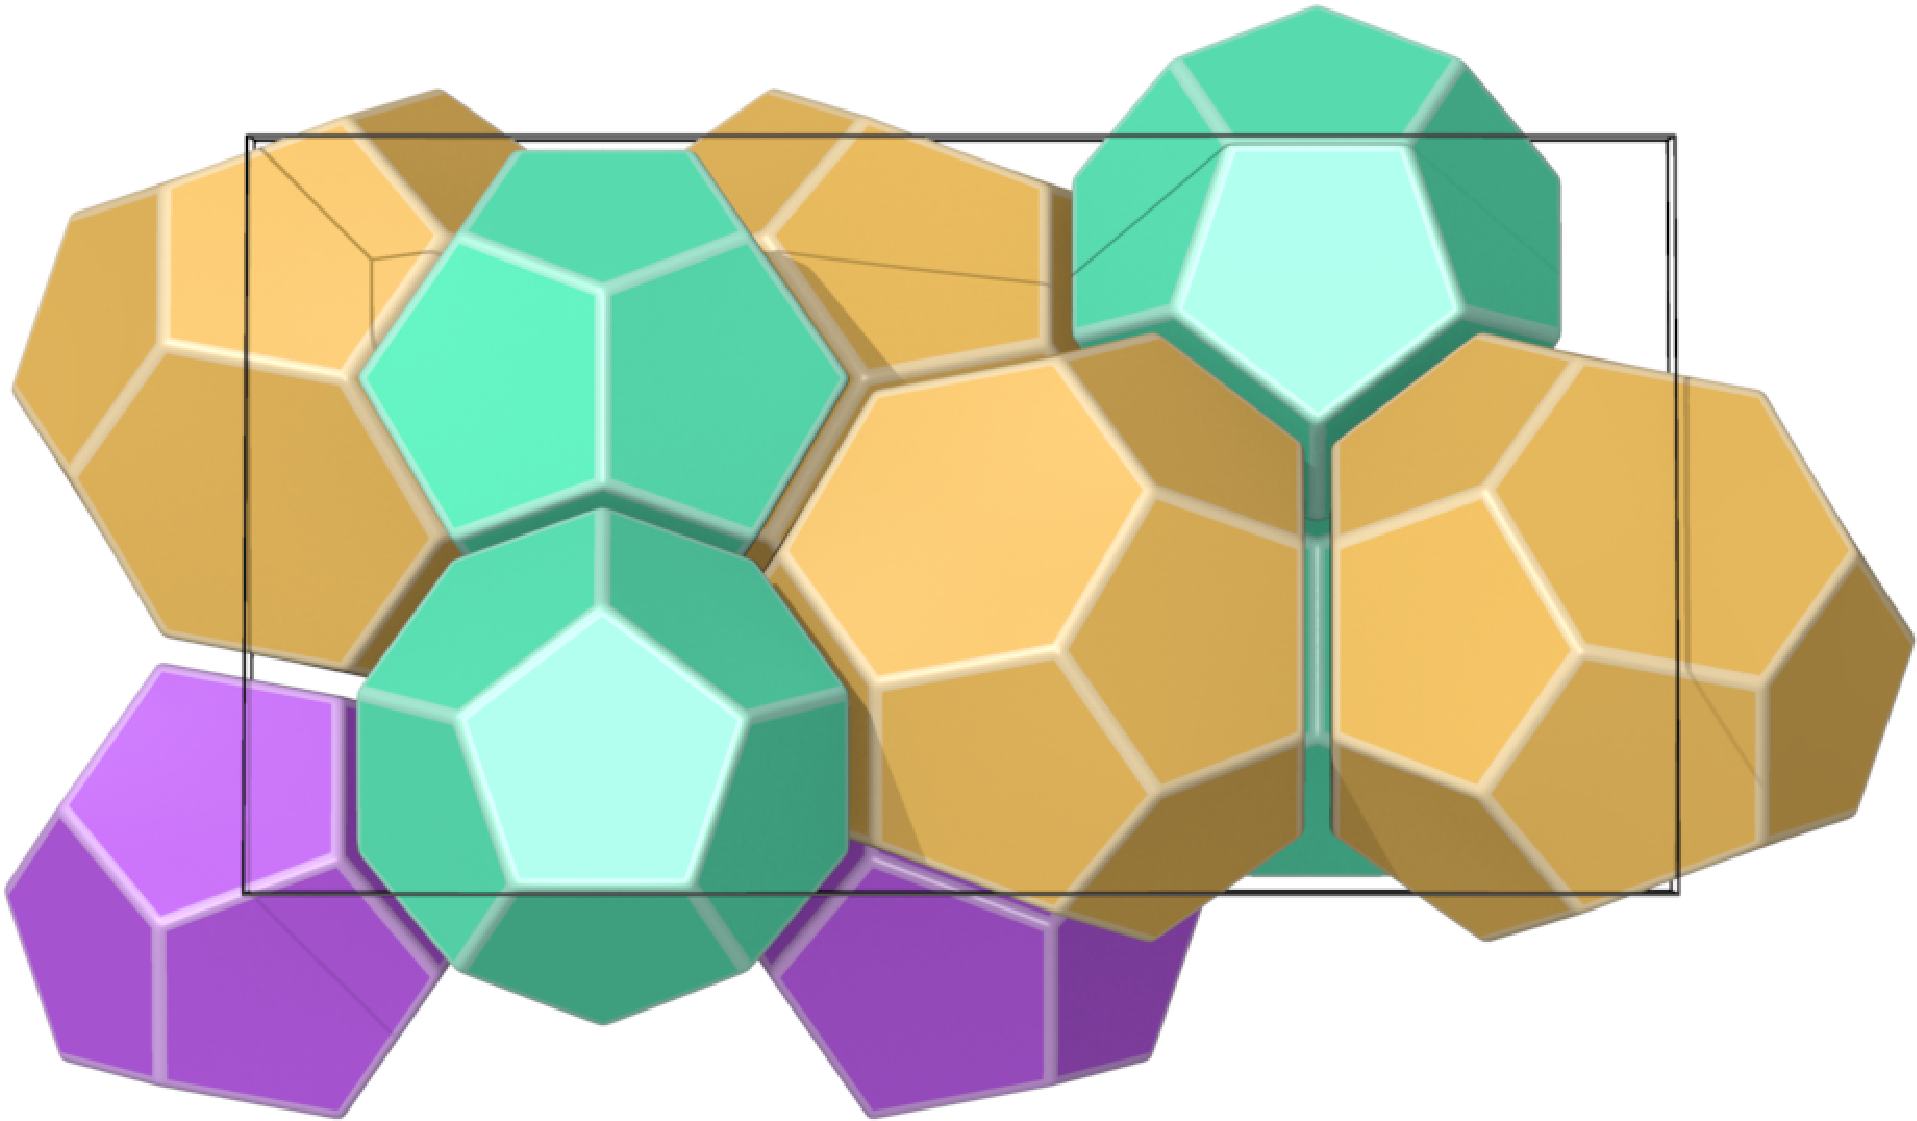
\epsfig{width=2.8cm, file=SpaceFullPicture/PIC20_84_V2/30_68-crop.pdf}\par
%\resizebox{2.8cm}{!}{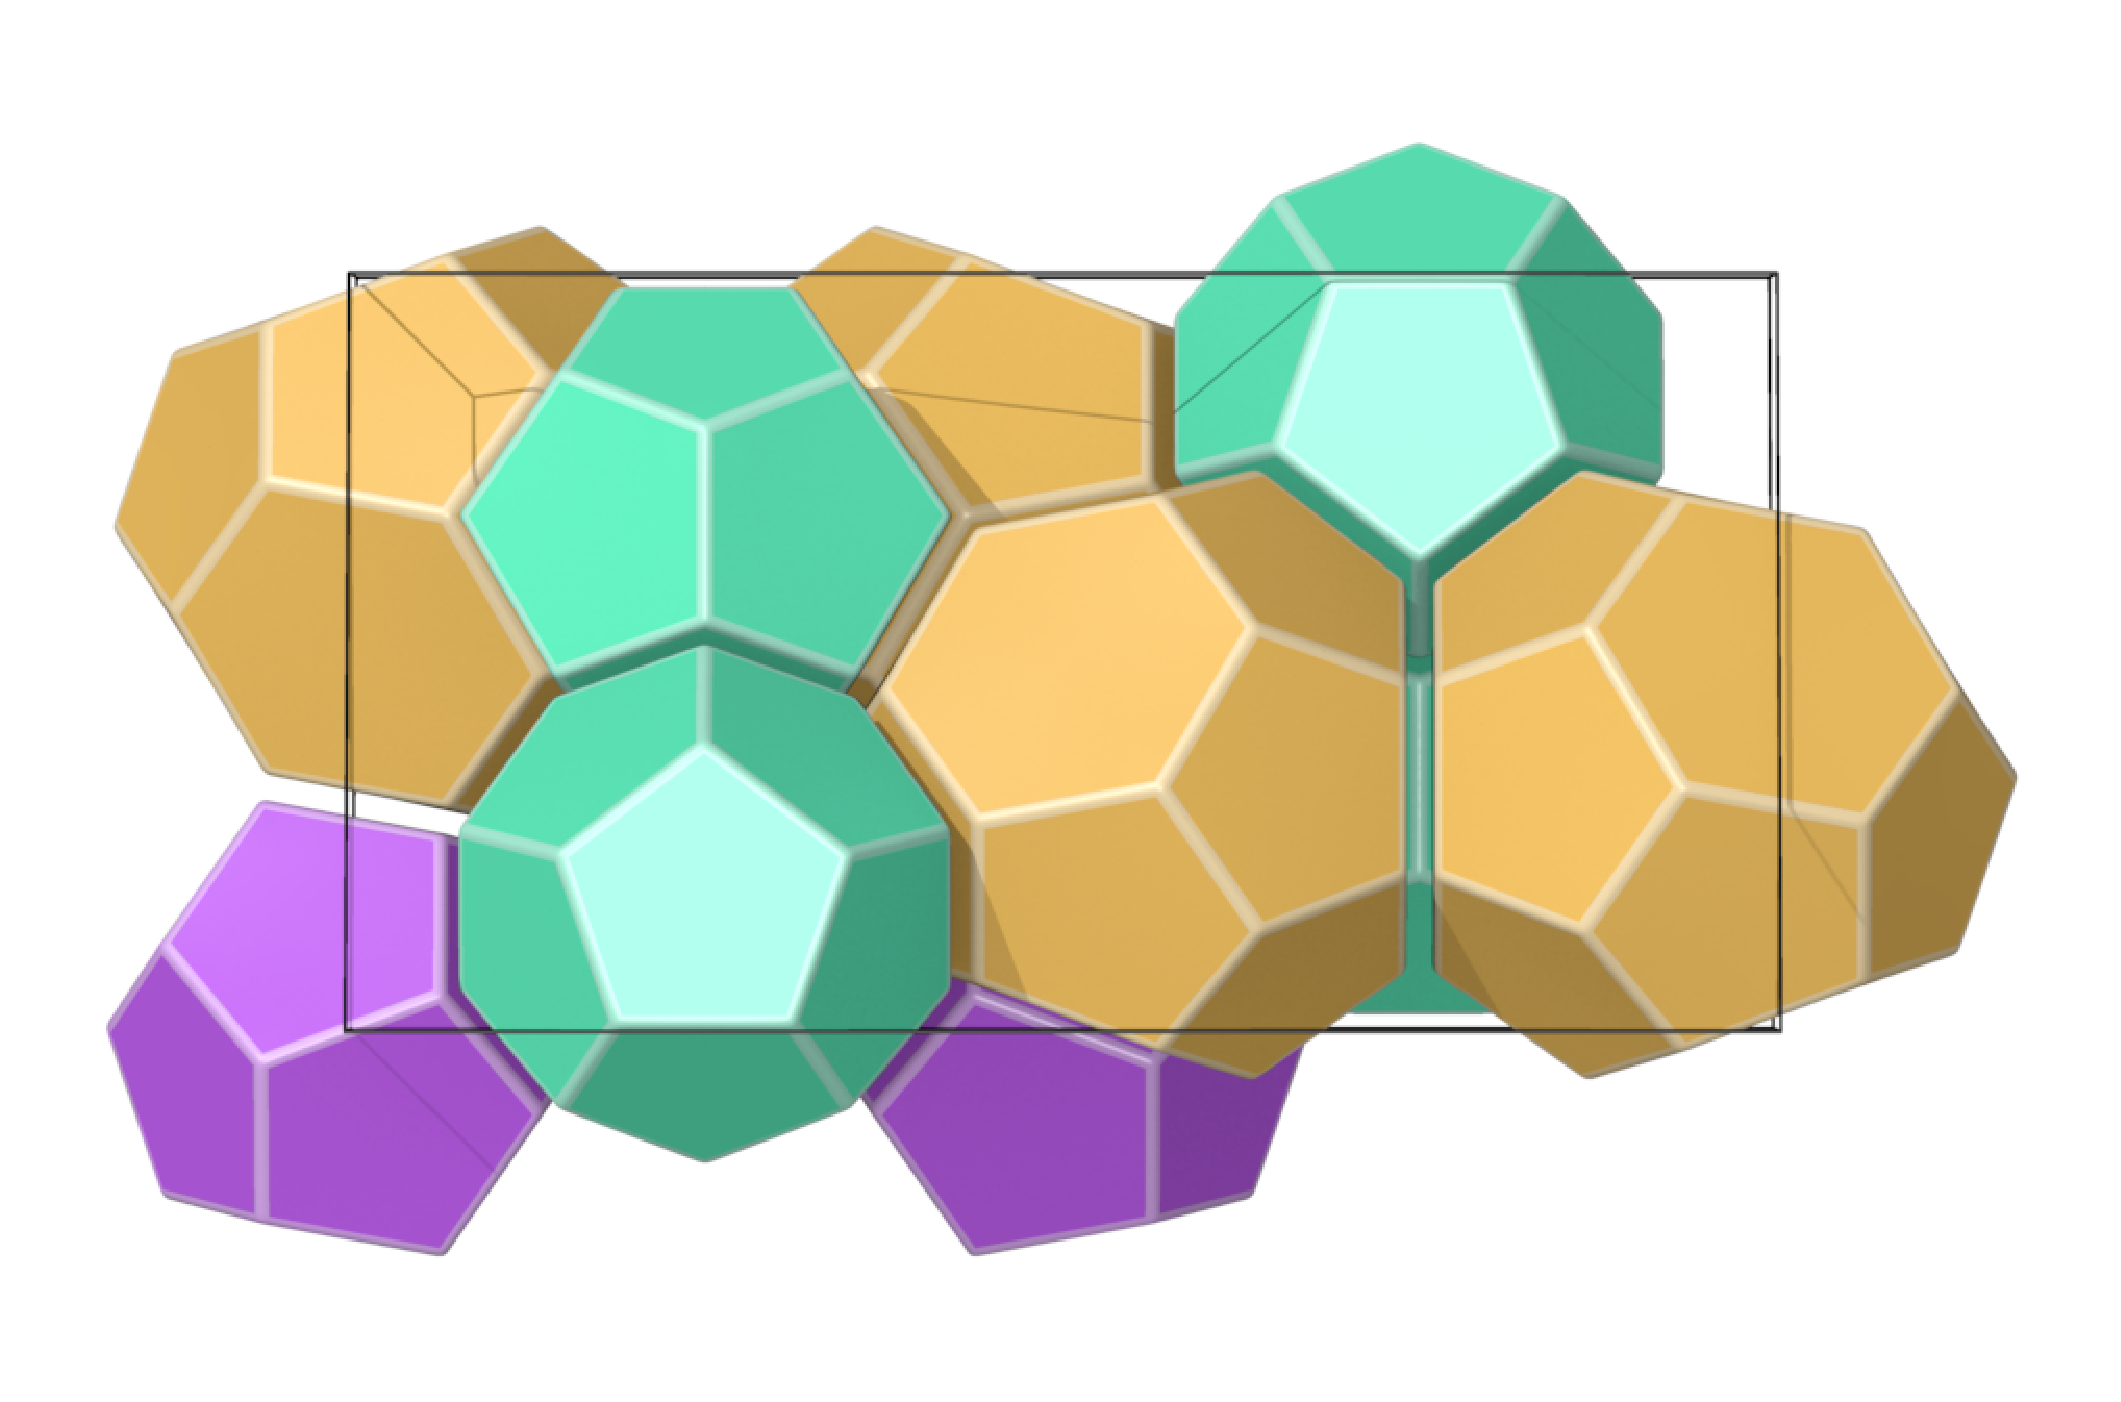
\includegraphics[bb=49 69 969 607,clip]{SpaceFullPicture/PIC20_84_V2/30_68.pdf}}\par
$P6_3/mmc$, $12$
\end{minipage}
\begin{minipage}[b]{3.1cm}
\centering
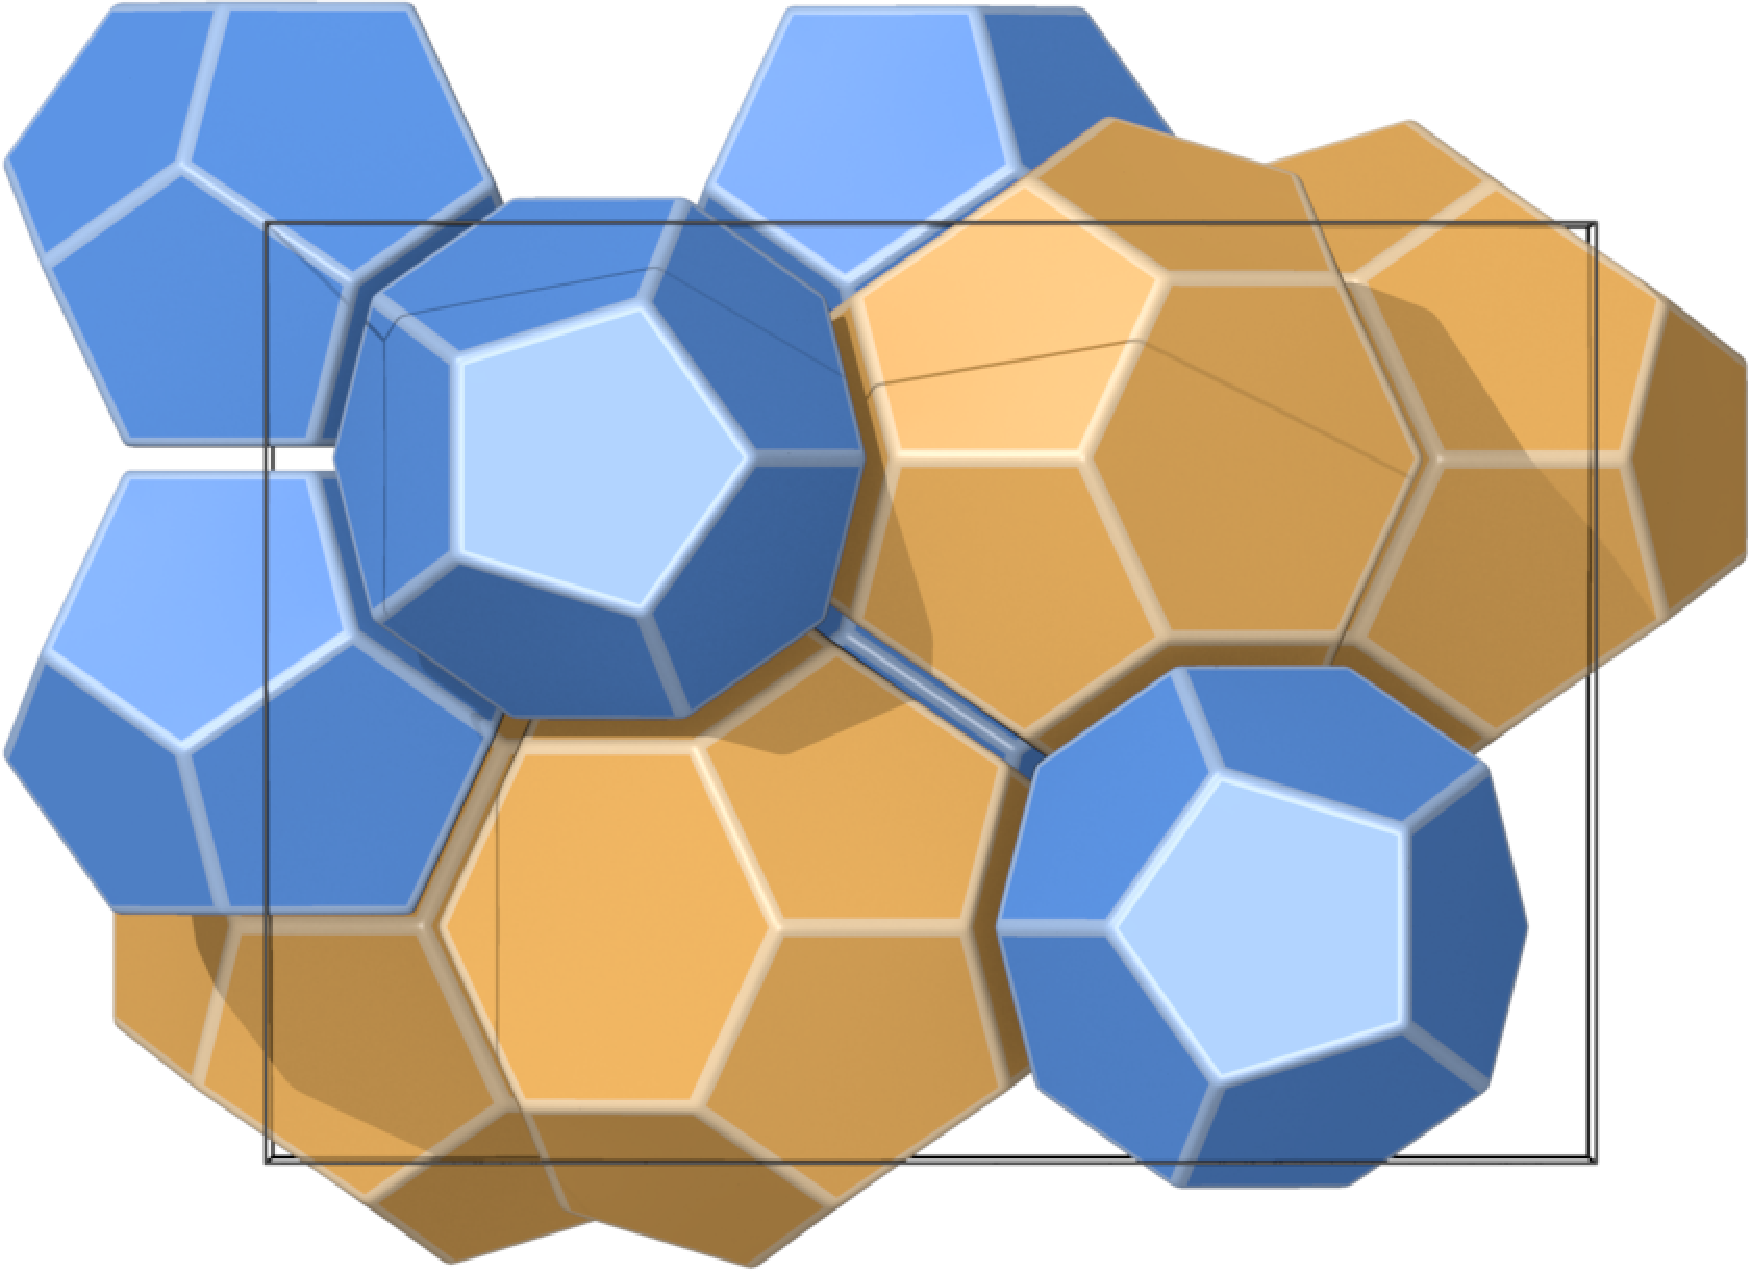
\epsfig{width=2.8cm, file=SpaceFullPicture/PIC20_84_V2/30_19-crop.pdf}\par
%\resizebox{2.8cm}{!}{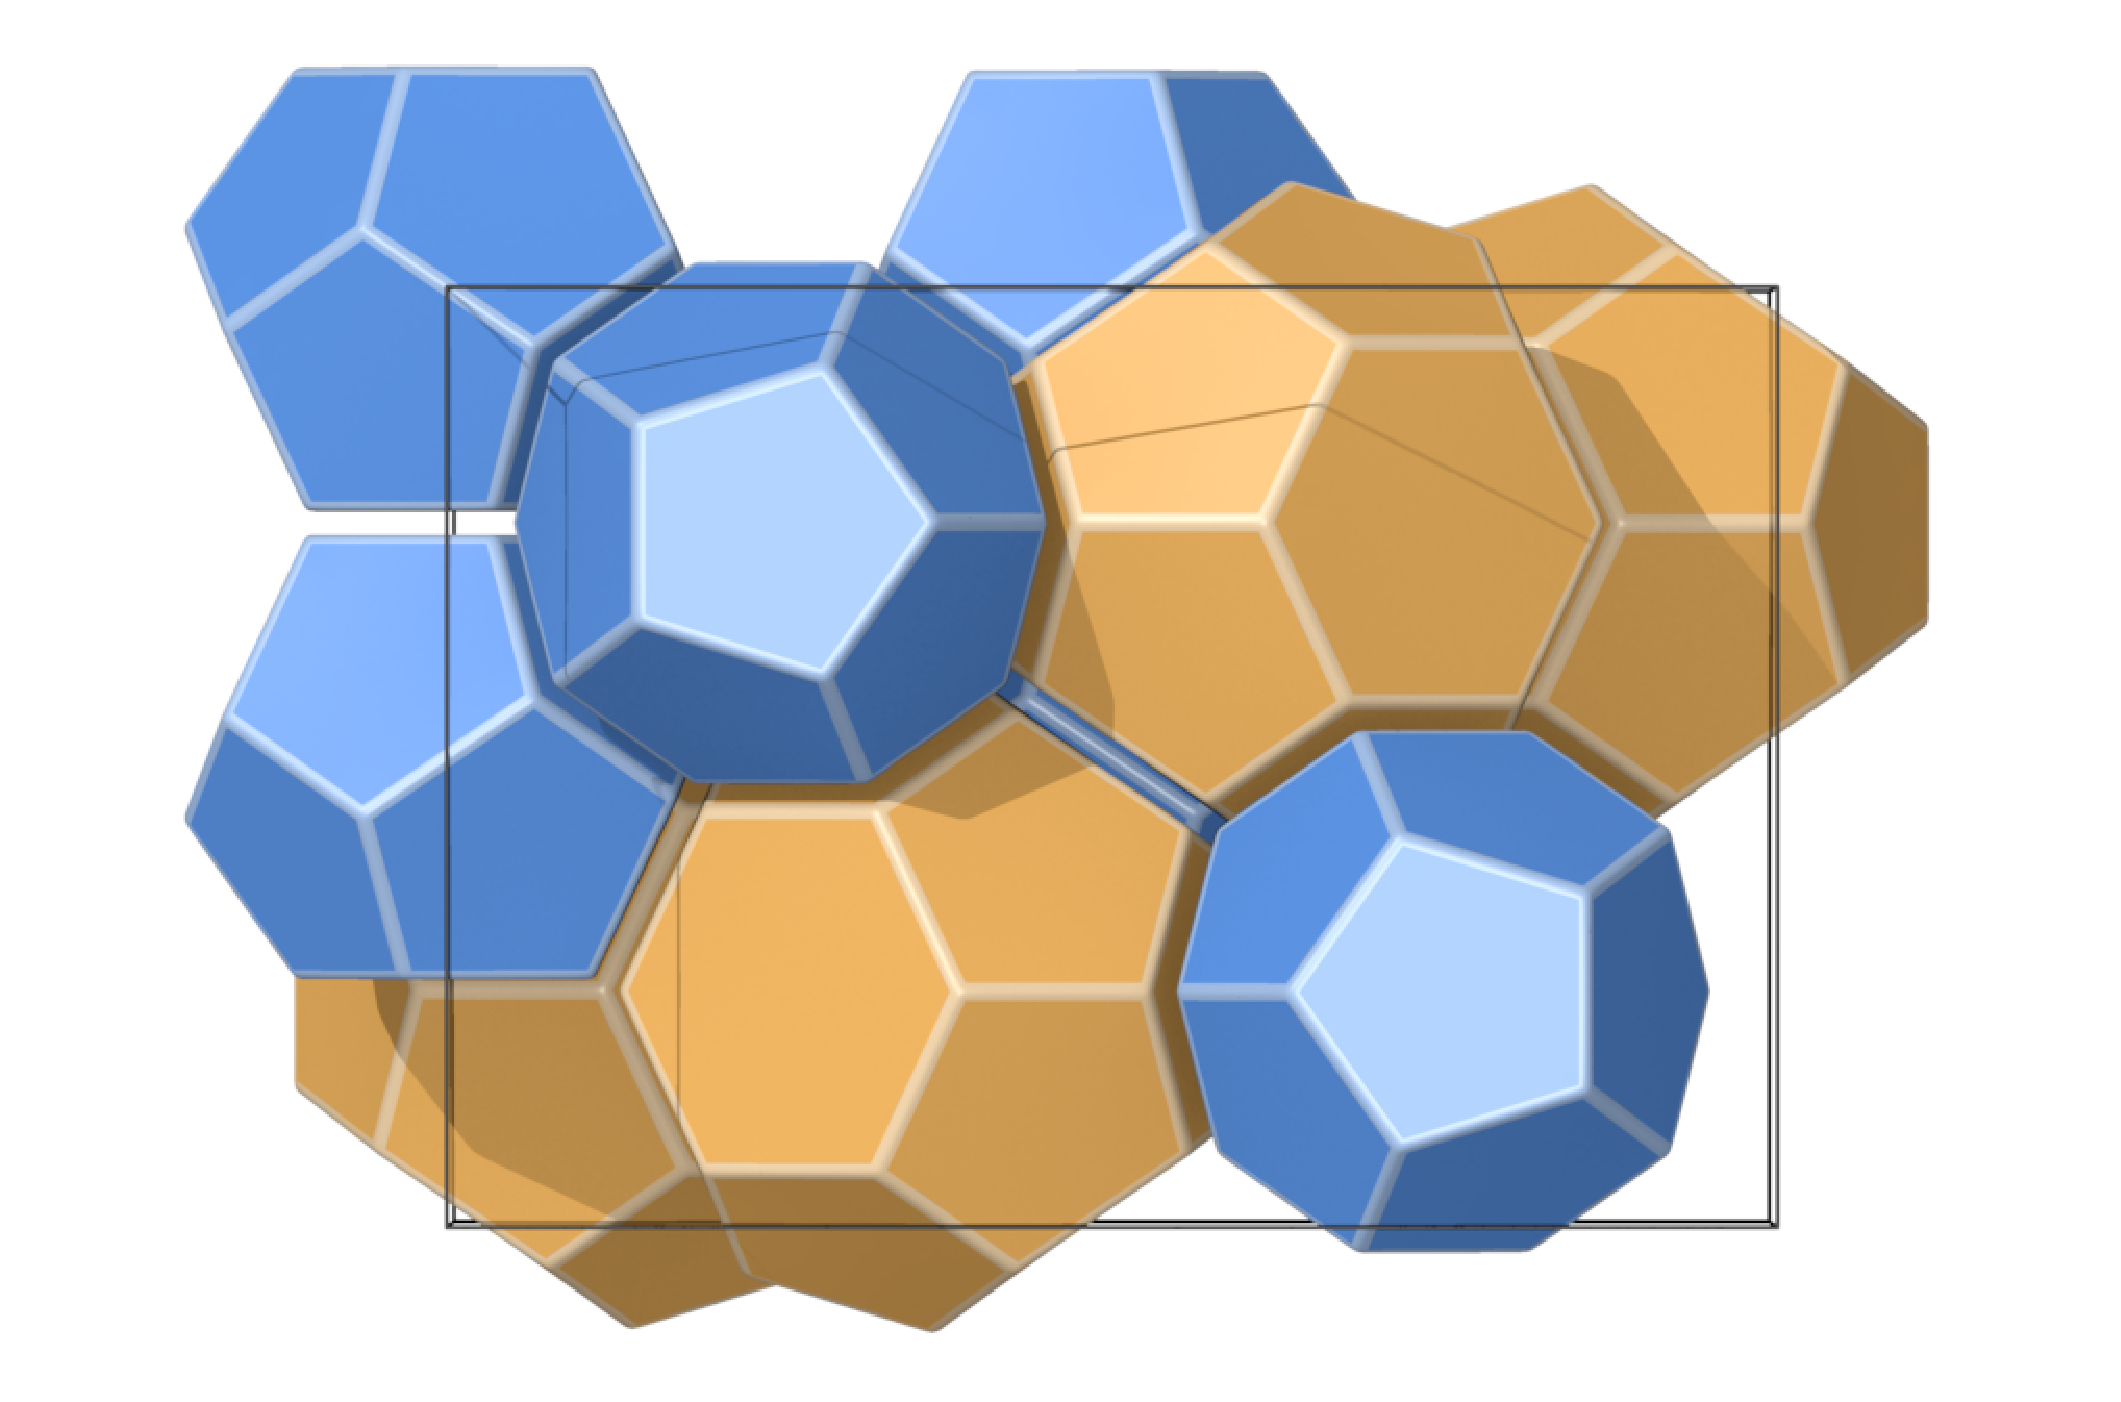
\includegraphics[bb=87 32 926 642, clip]{SpaceFullPicture/PIC20_84_V2/30_19.pdf}}\par
$Fd\overline{3}m$, $24$
\end{minipage}
\begin{minipage}[b]{3.1cm}
\centering
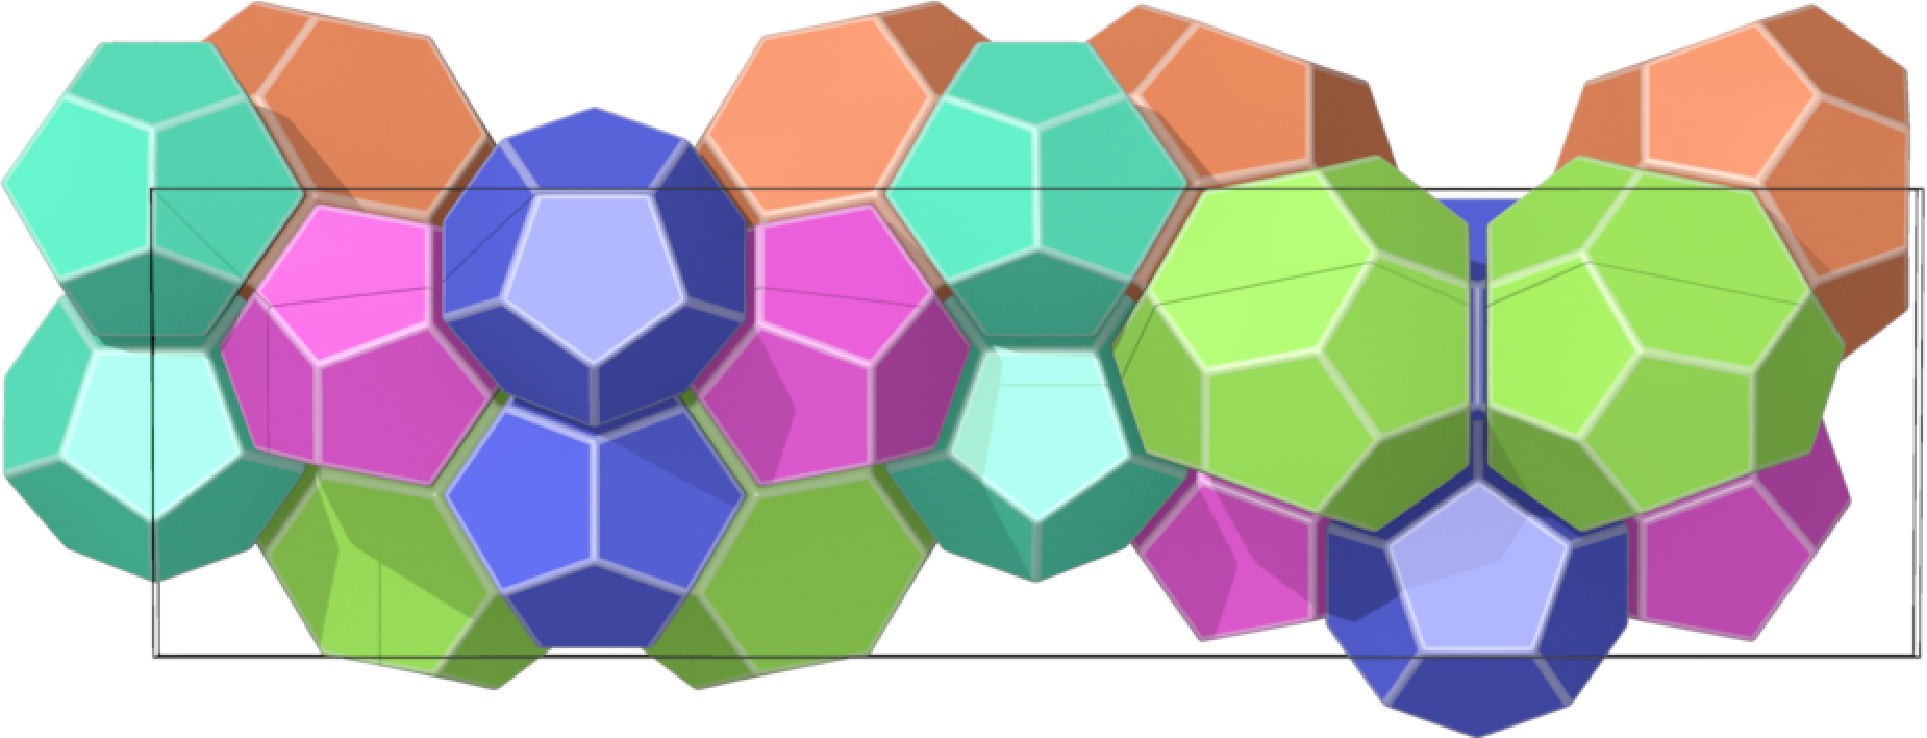
\epsfig{width=2.8cm, file=SpaceFullPicture/PIC20_84_V2/30_04-crop.pdf}\par
%\resizebox{2.8cm}{!}{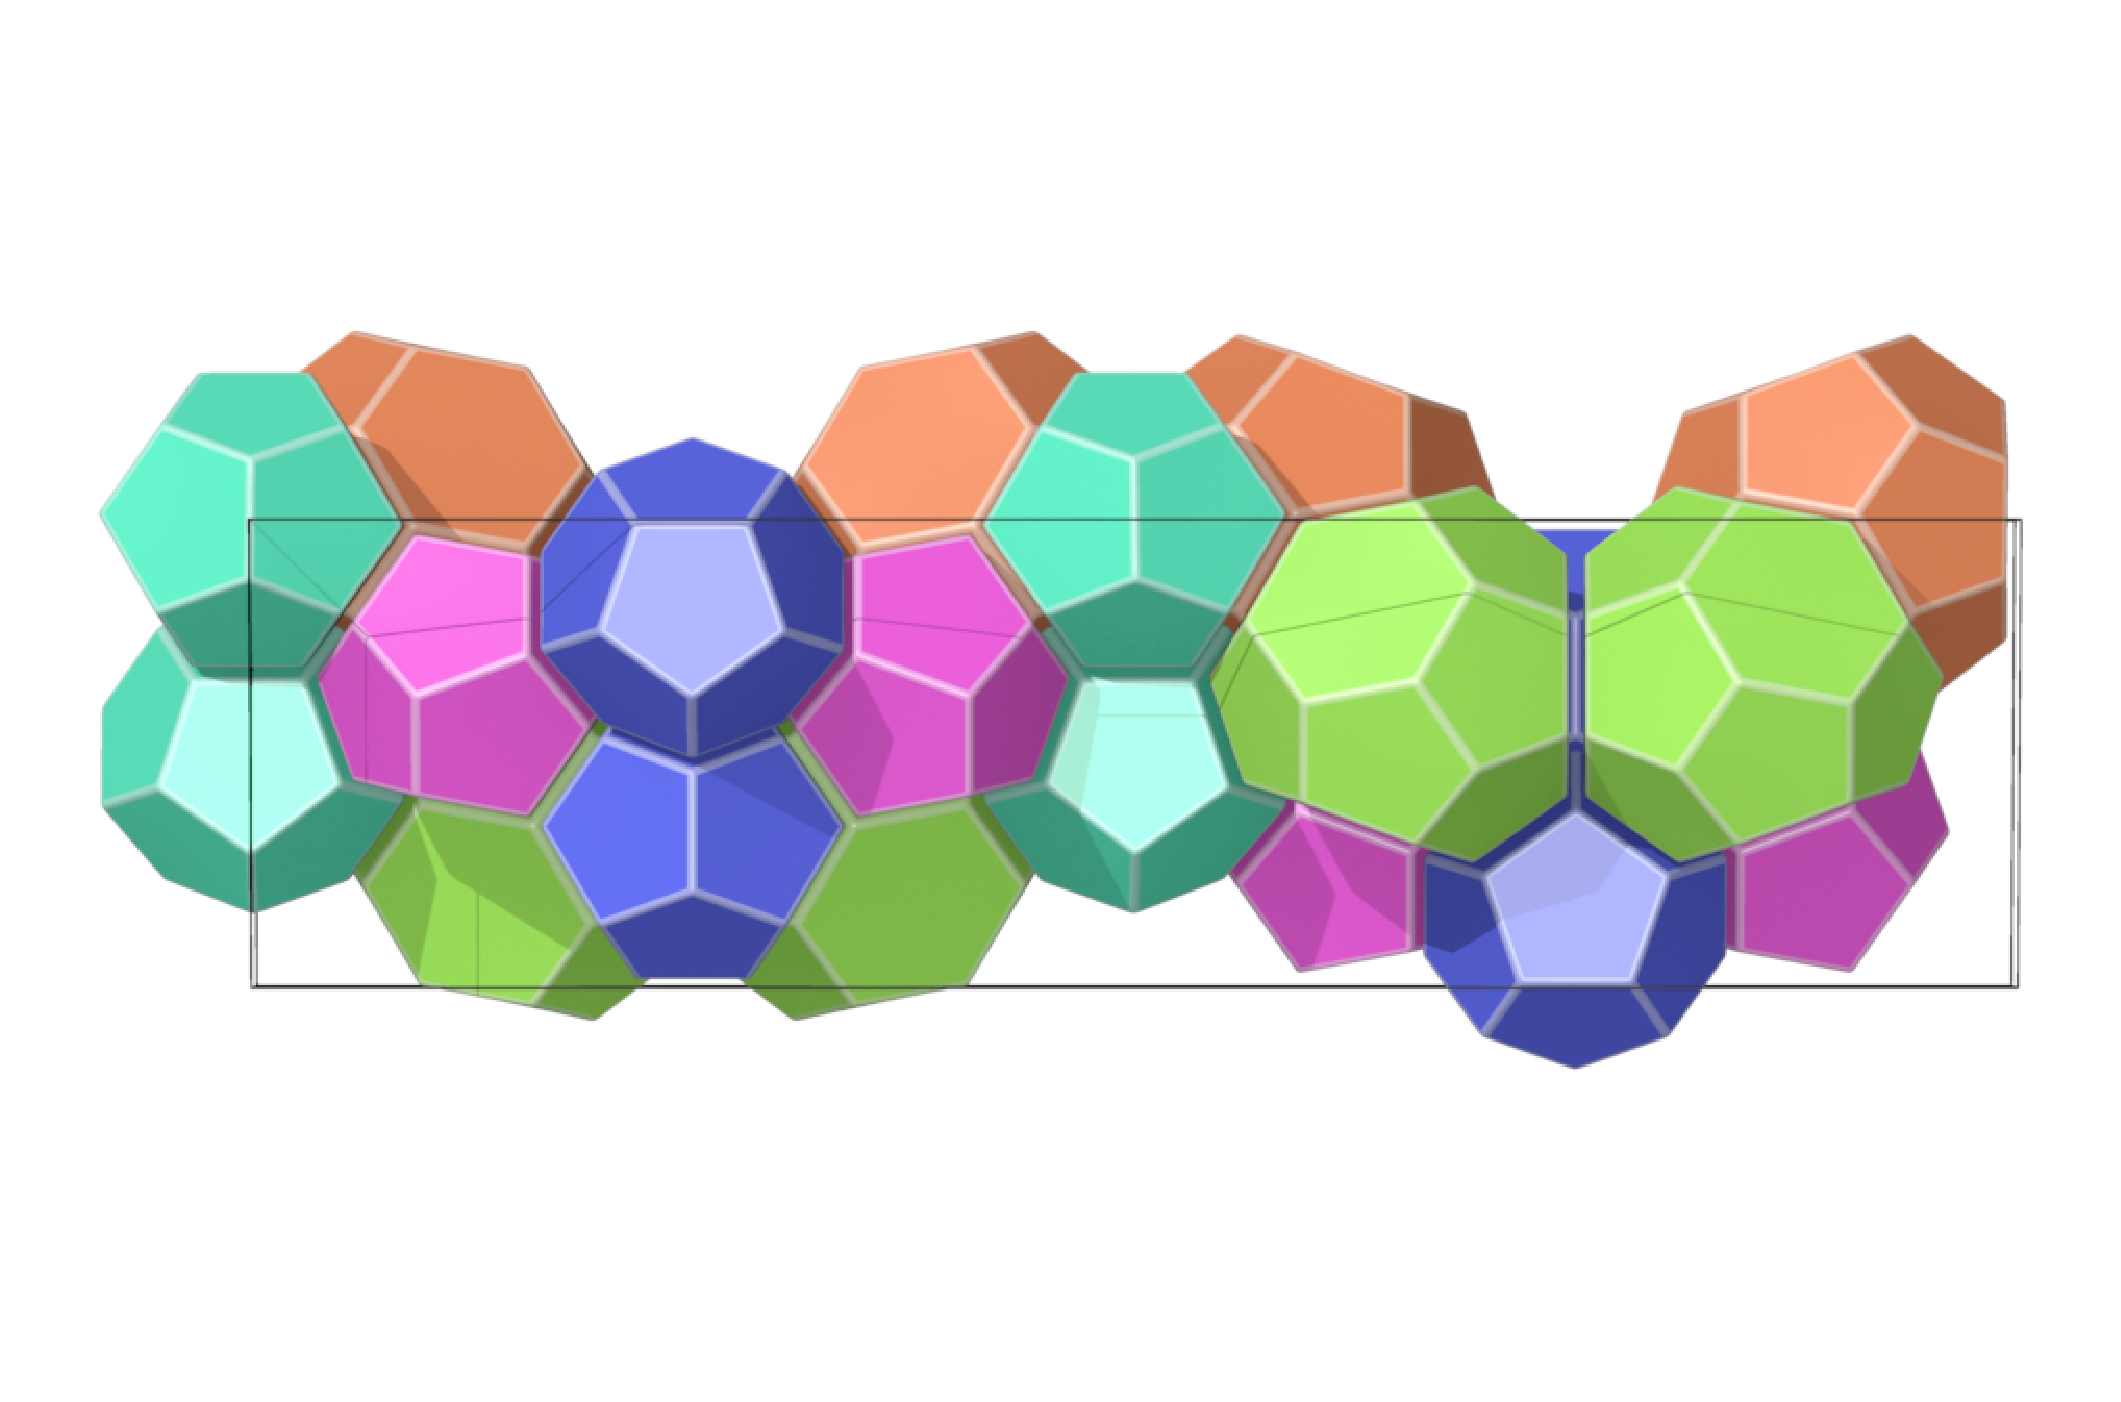
\includegraphics[bb=47 160 972 514, clip]{SpaceFullPicture/PIC20_84_V2/30_04.pdf}}\par
$P6_3/mmc$, $24$
\end{minipage}
\begin{minipage}[b]{3.1cm}
\centering
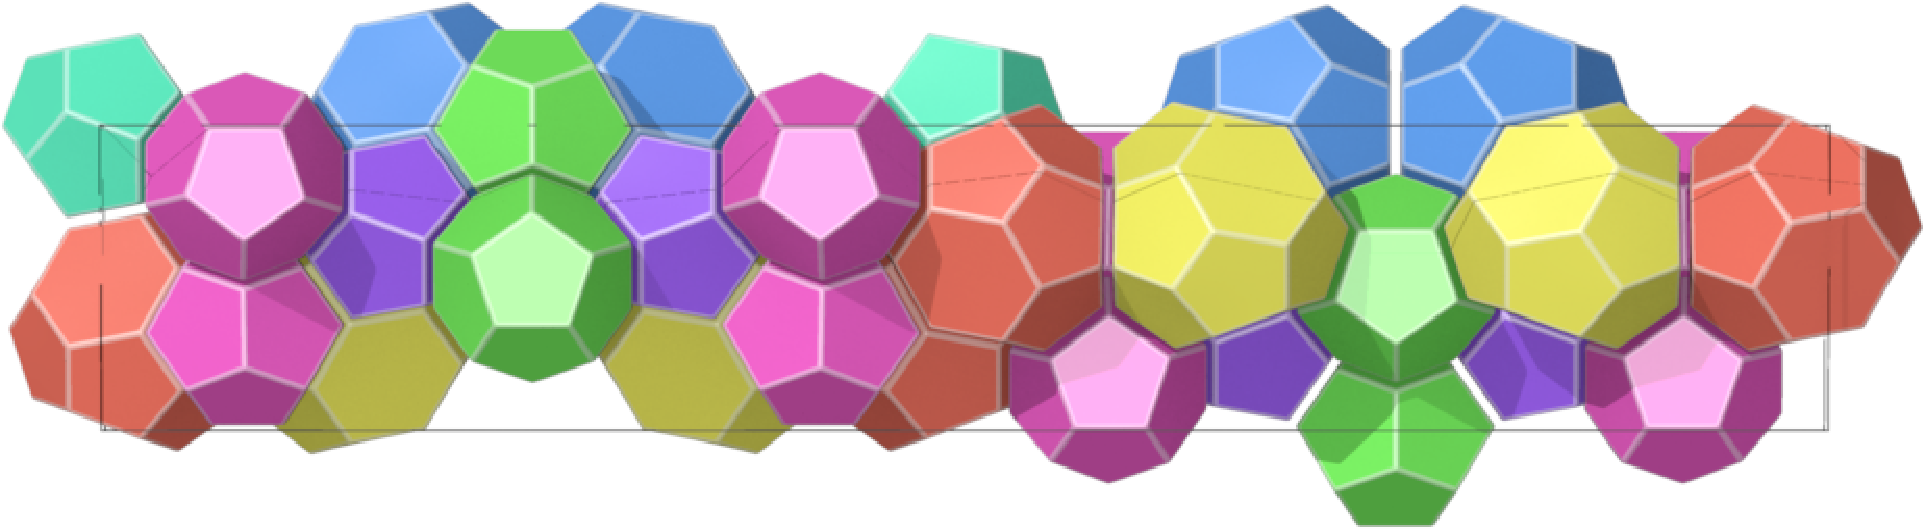
\epsfig{width=2.8cm, file=SpaceFullPicture/PIC20_84_V2/30_24-crop.pdf}\par
%\resizebox{2.8cm}{!}{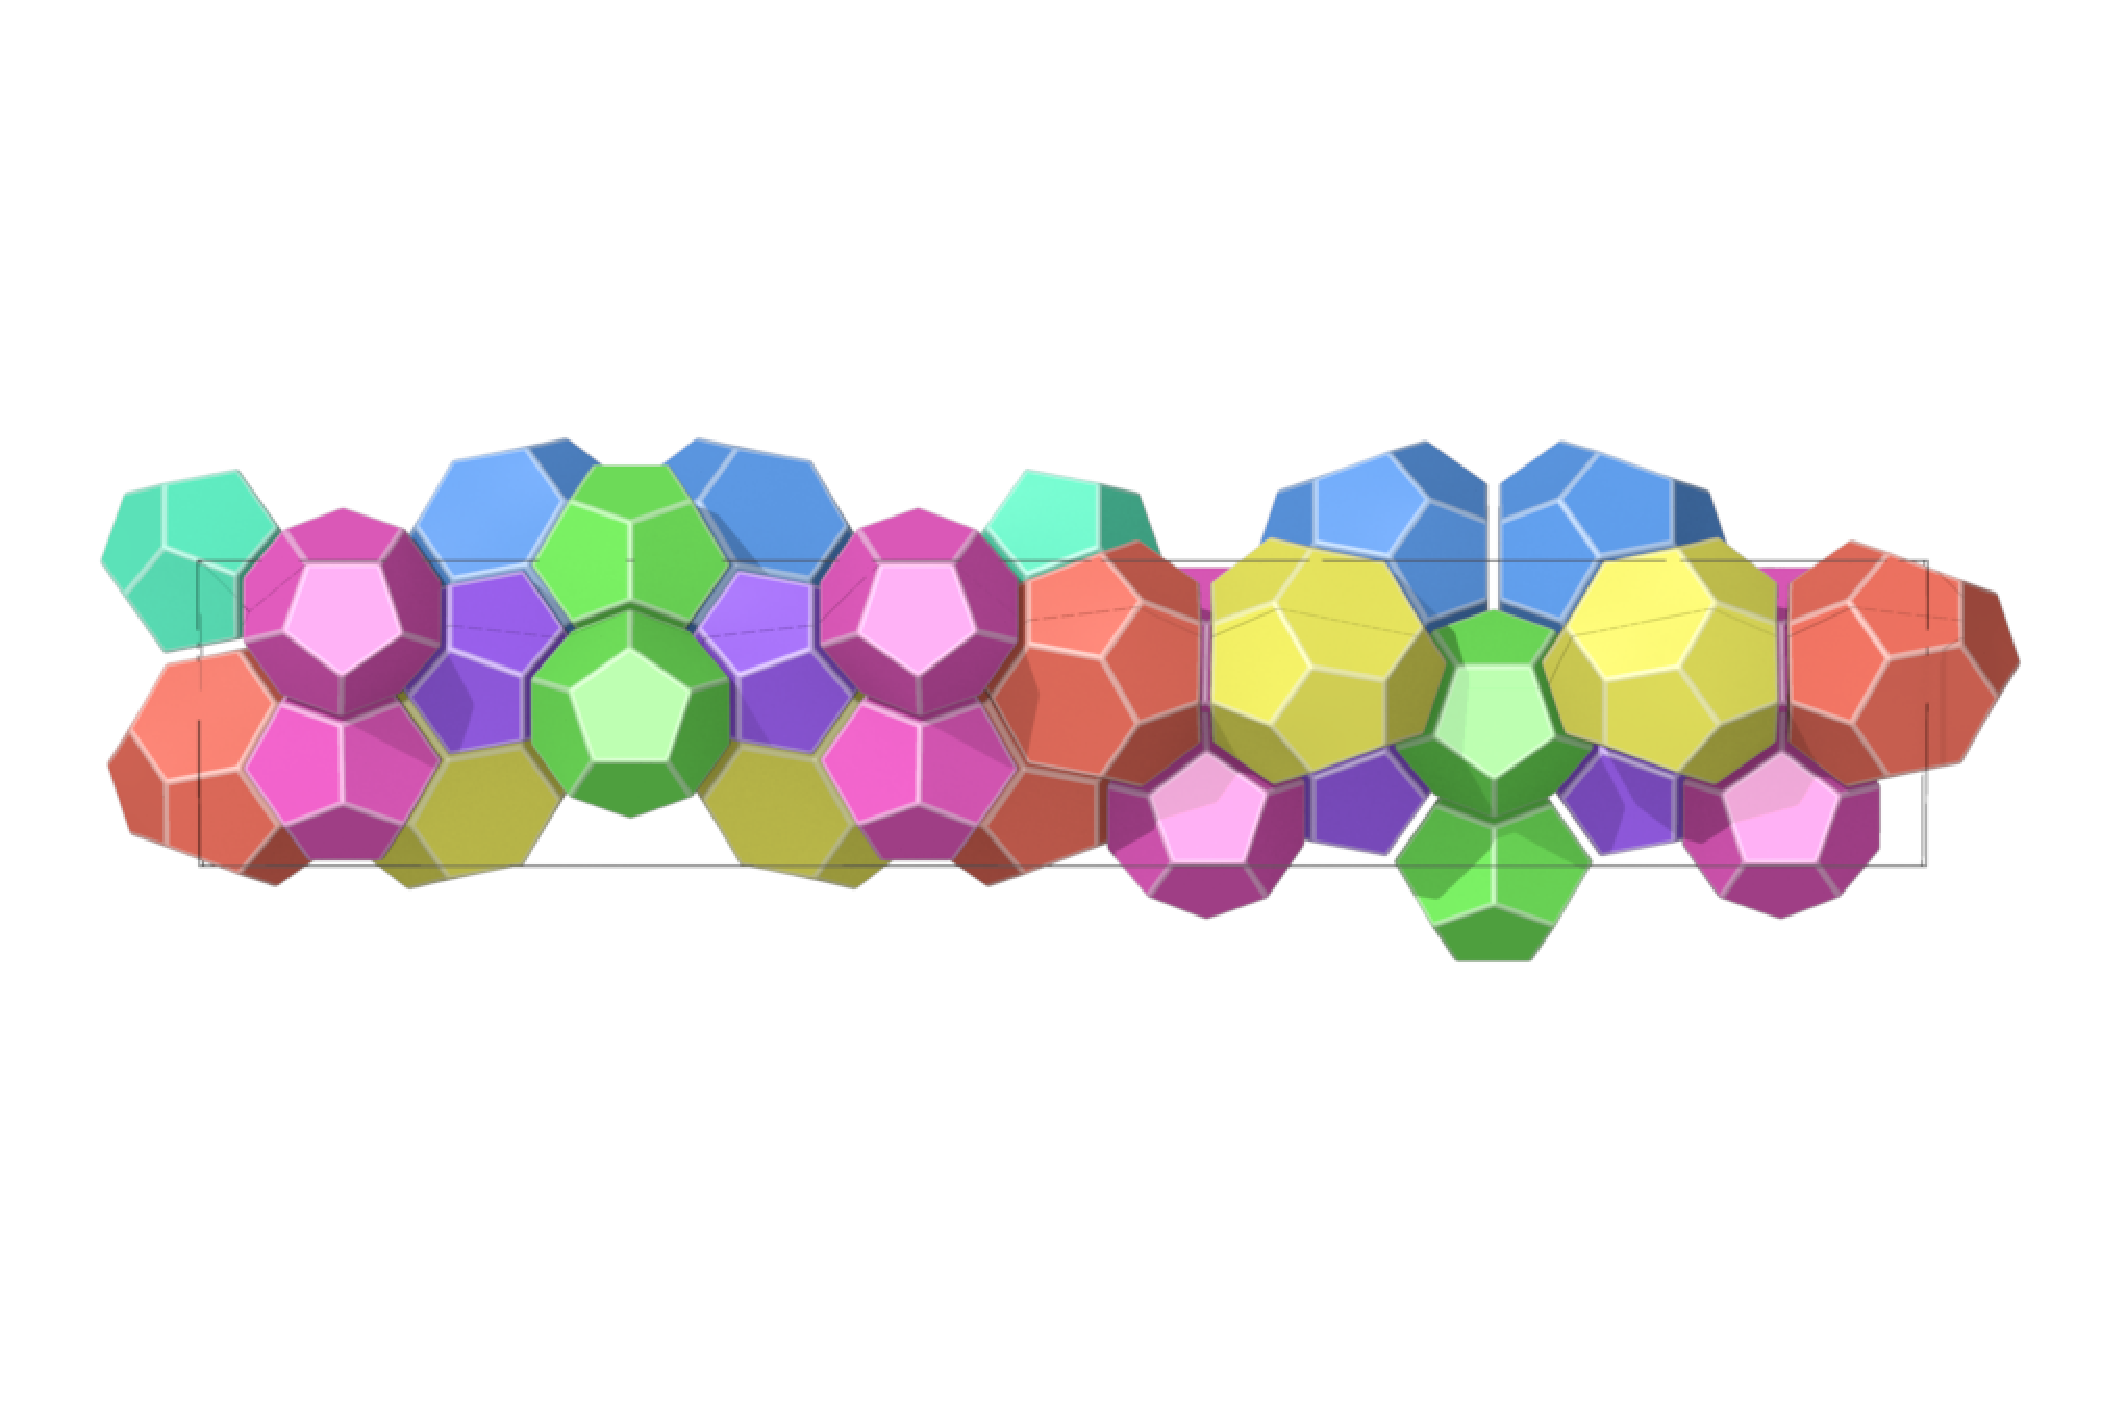
\includegraphics[bb=47 210 970 464, clip]{SpaceFullPicture/PIC20_84_V2/30_24.pdf}}\par
$P6_3/mmc$, $36$
\end{minipage}
\begin{minipage}[b]{3.1cm}
\centering
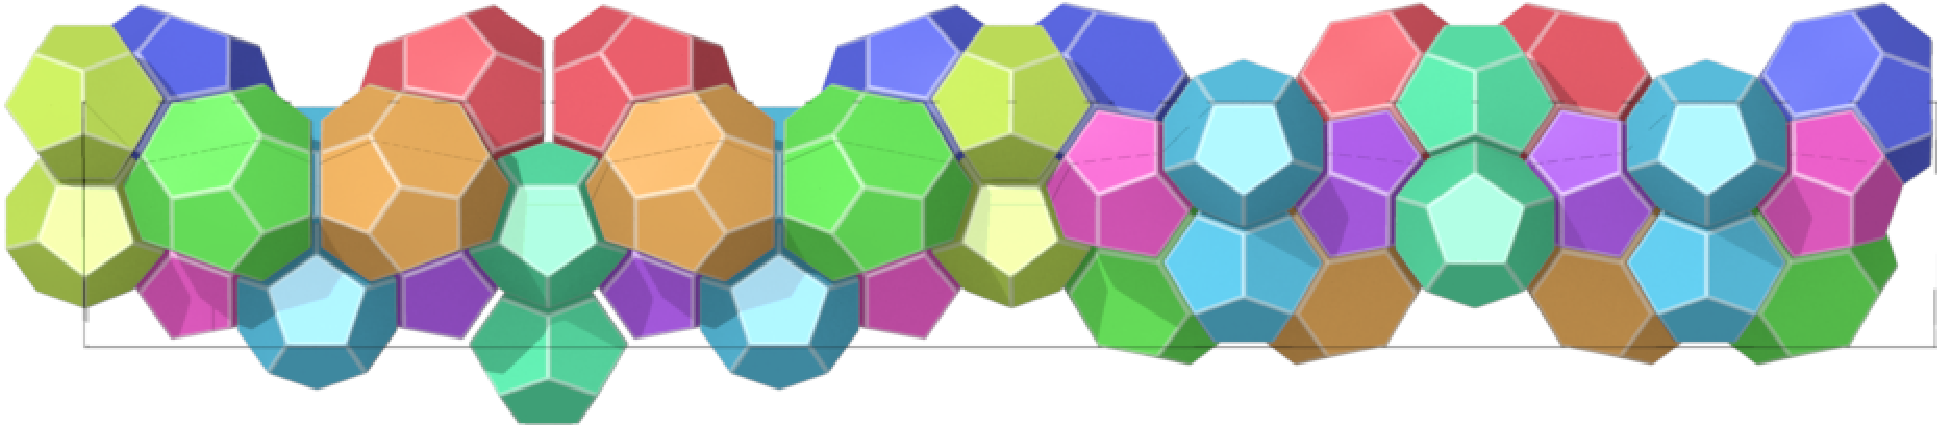
\epsfig{width=2.8cm, file=SpaceFullPicture/PHYS/MgZn2_0d03MgAg2-crop.pdf}\par
%\resizebox{2.8cm}{!}{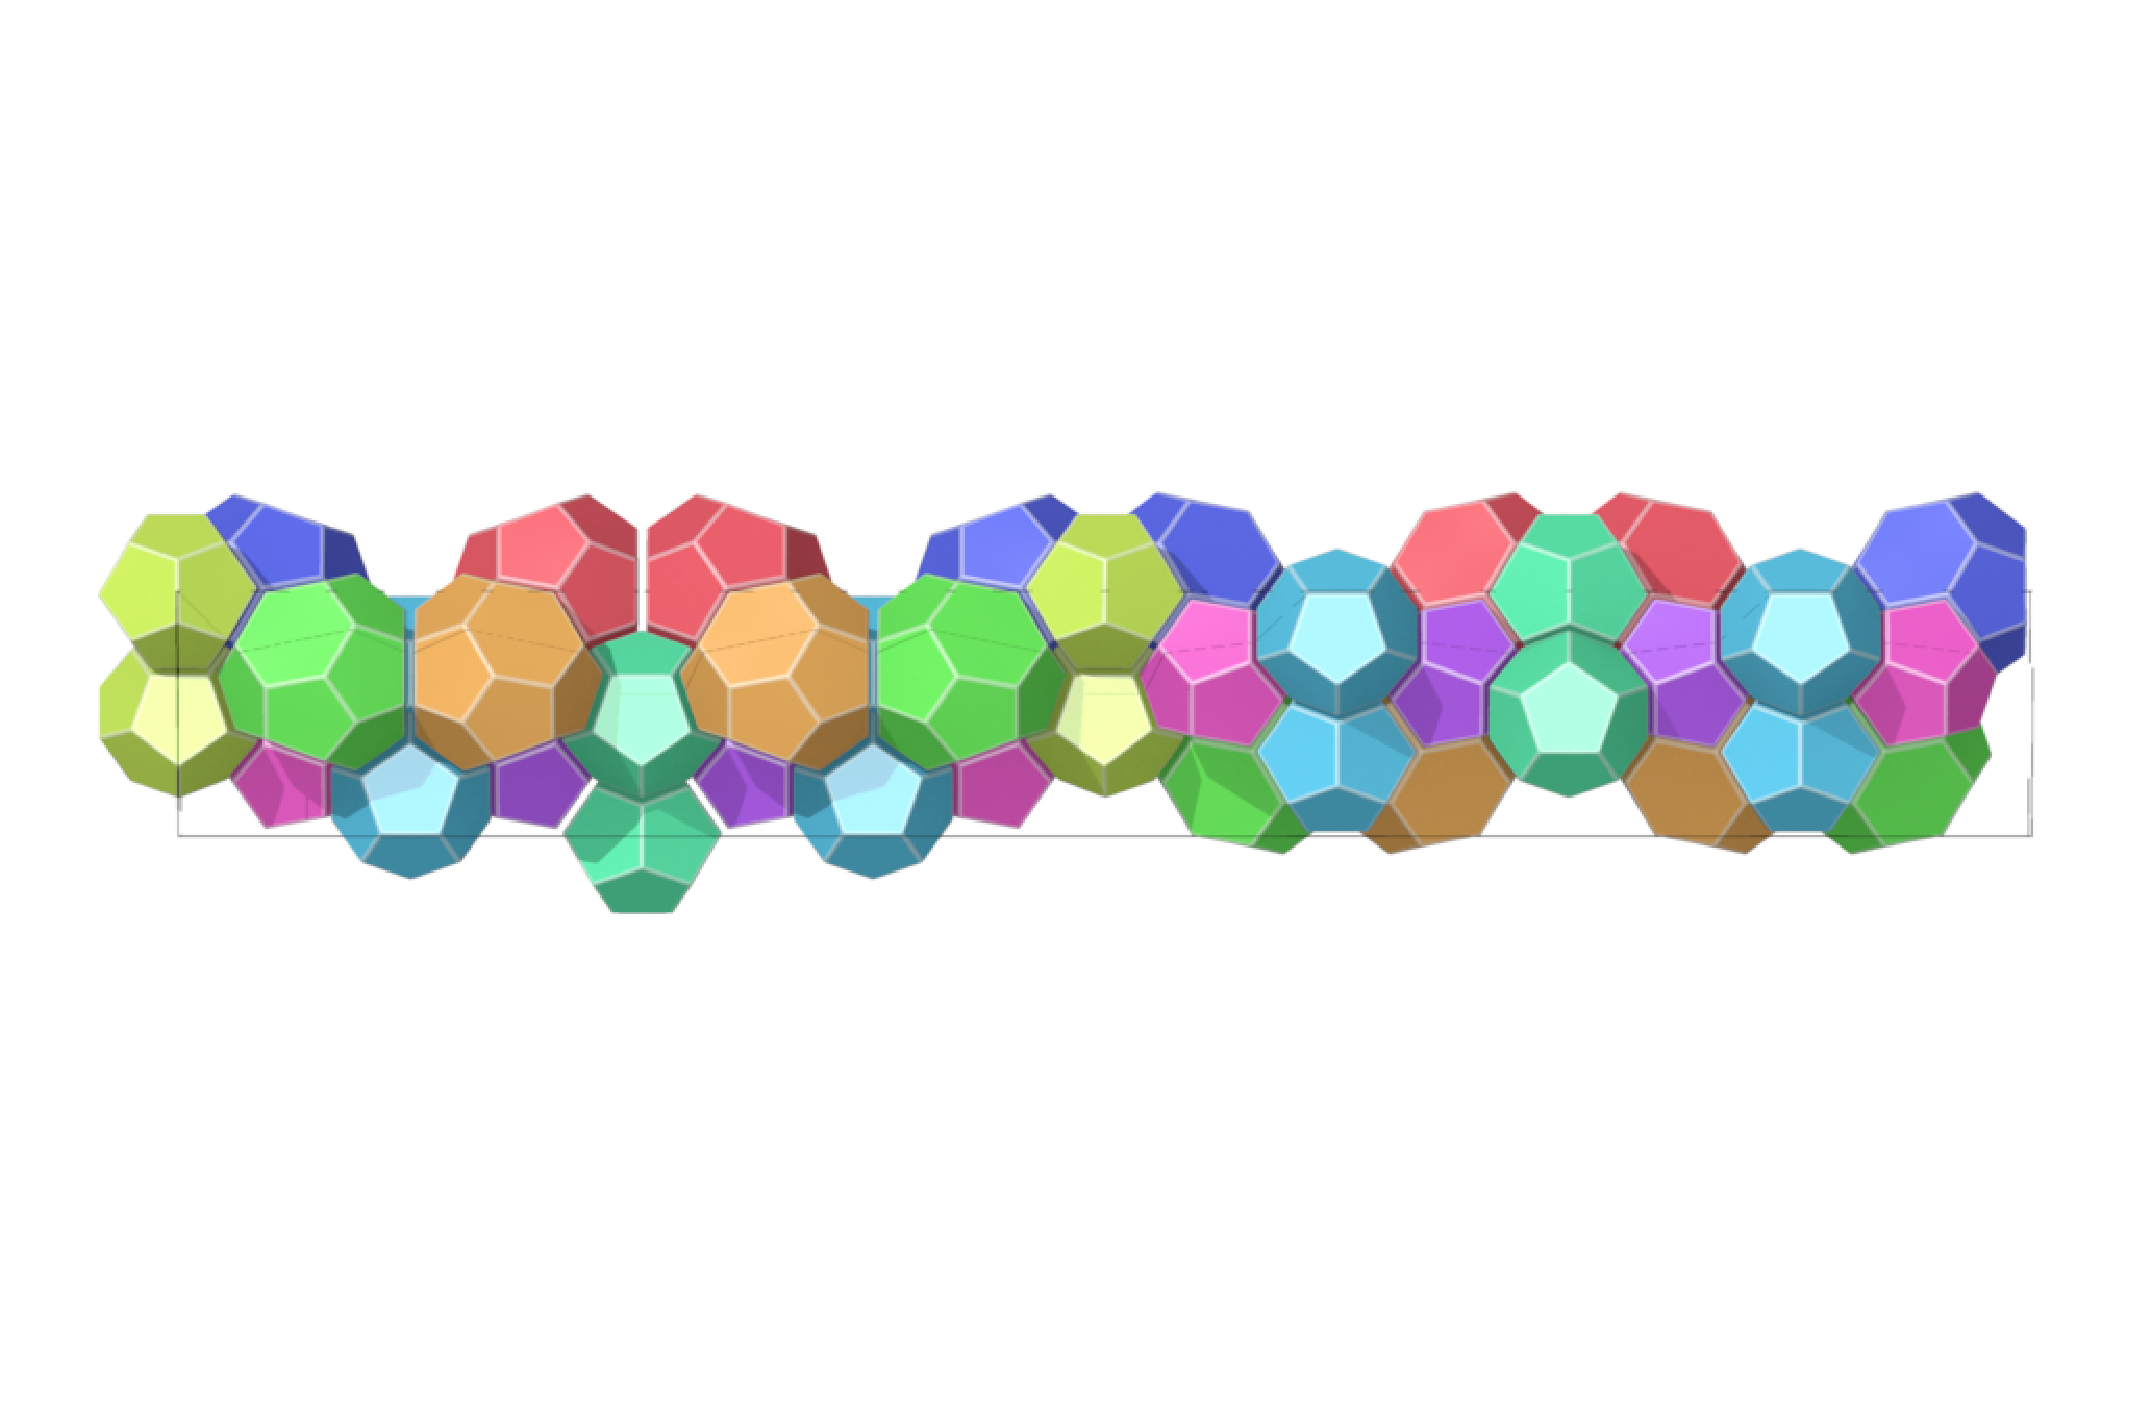
\includegraphics[bb=45 237 975 441, clip]{SpaceFullPicture/PHYS/MgZn2_0d03MgAg2.pdf}}\par
$P6_3/mmc$, $48$
\end{minipage}
\begin{minipage}[b]{3.1cm}
\centering
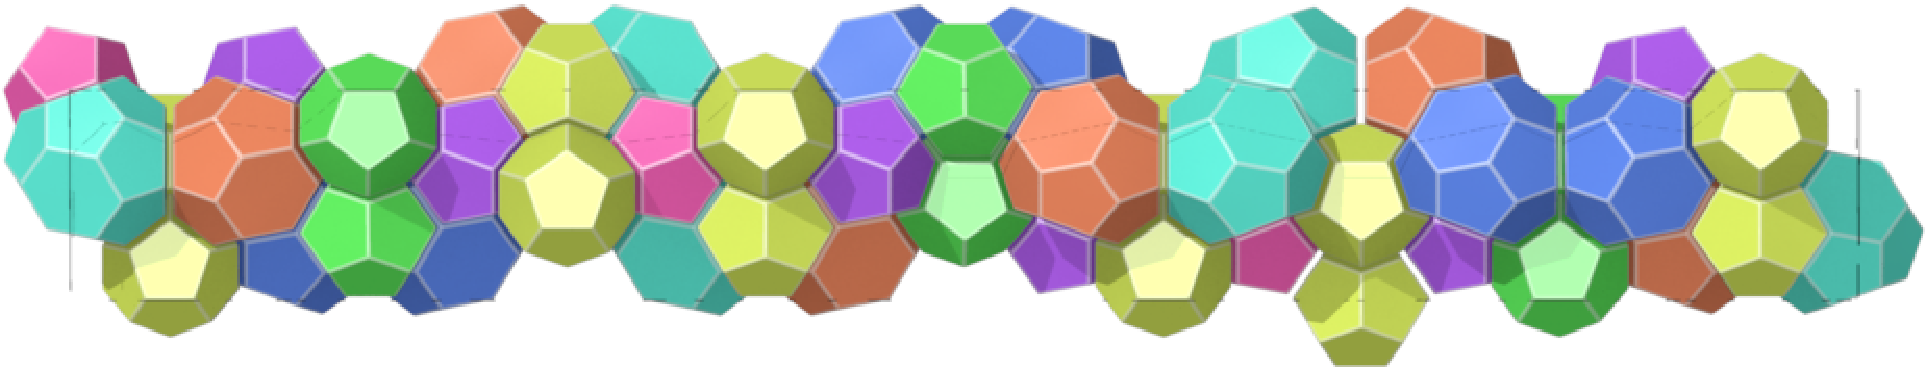
\epsfig{width=2.8cm, file=SpaceFullPicture/PIC20_84_V2/30_25-crop.pdf}\par
%\resizebox{2.8cm}{!}{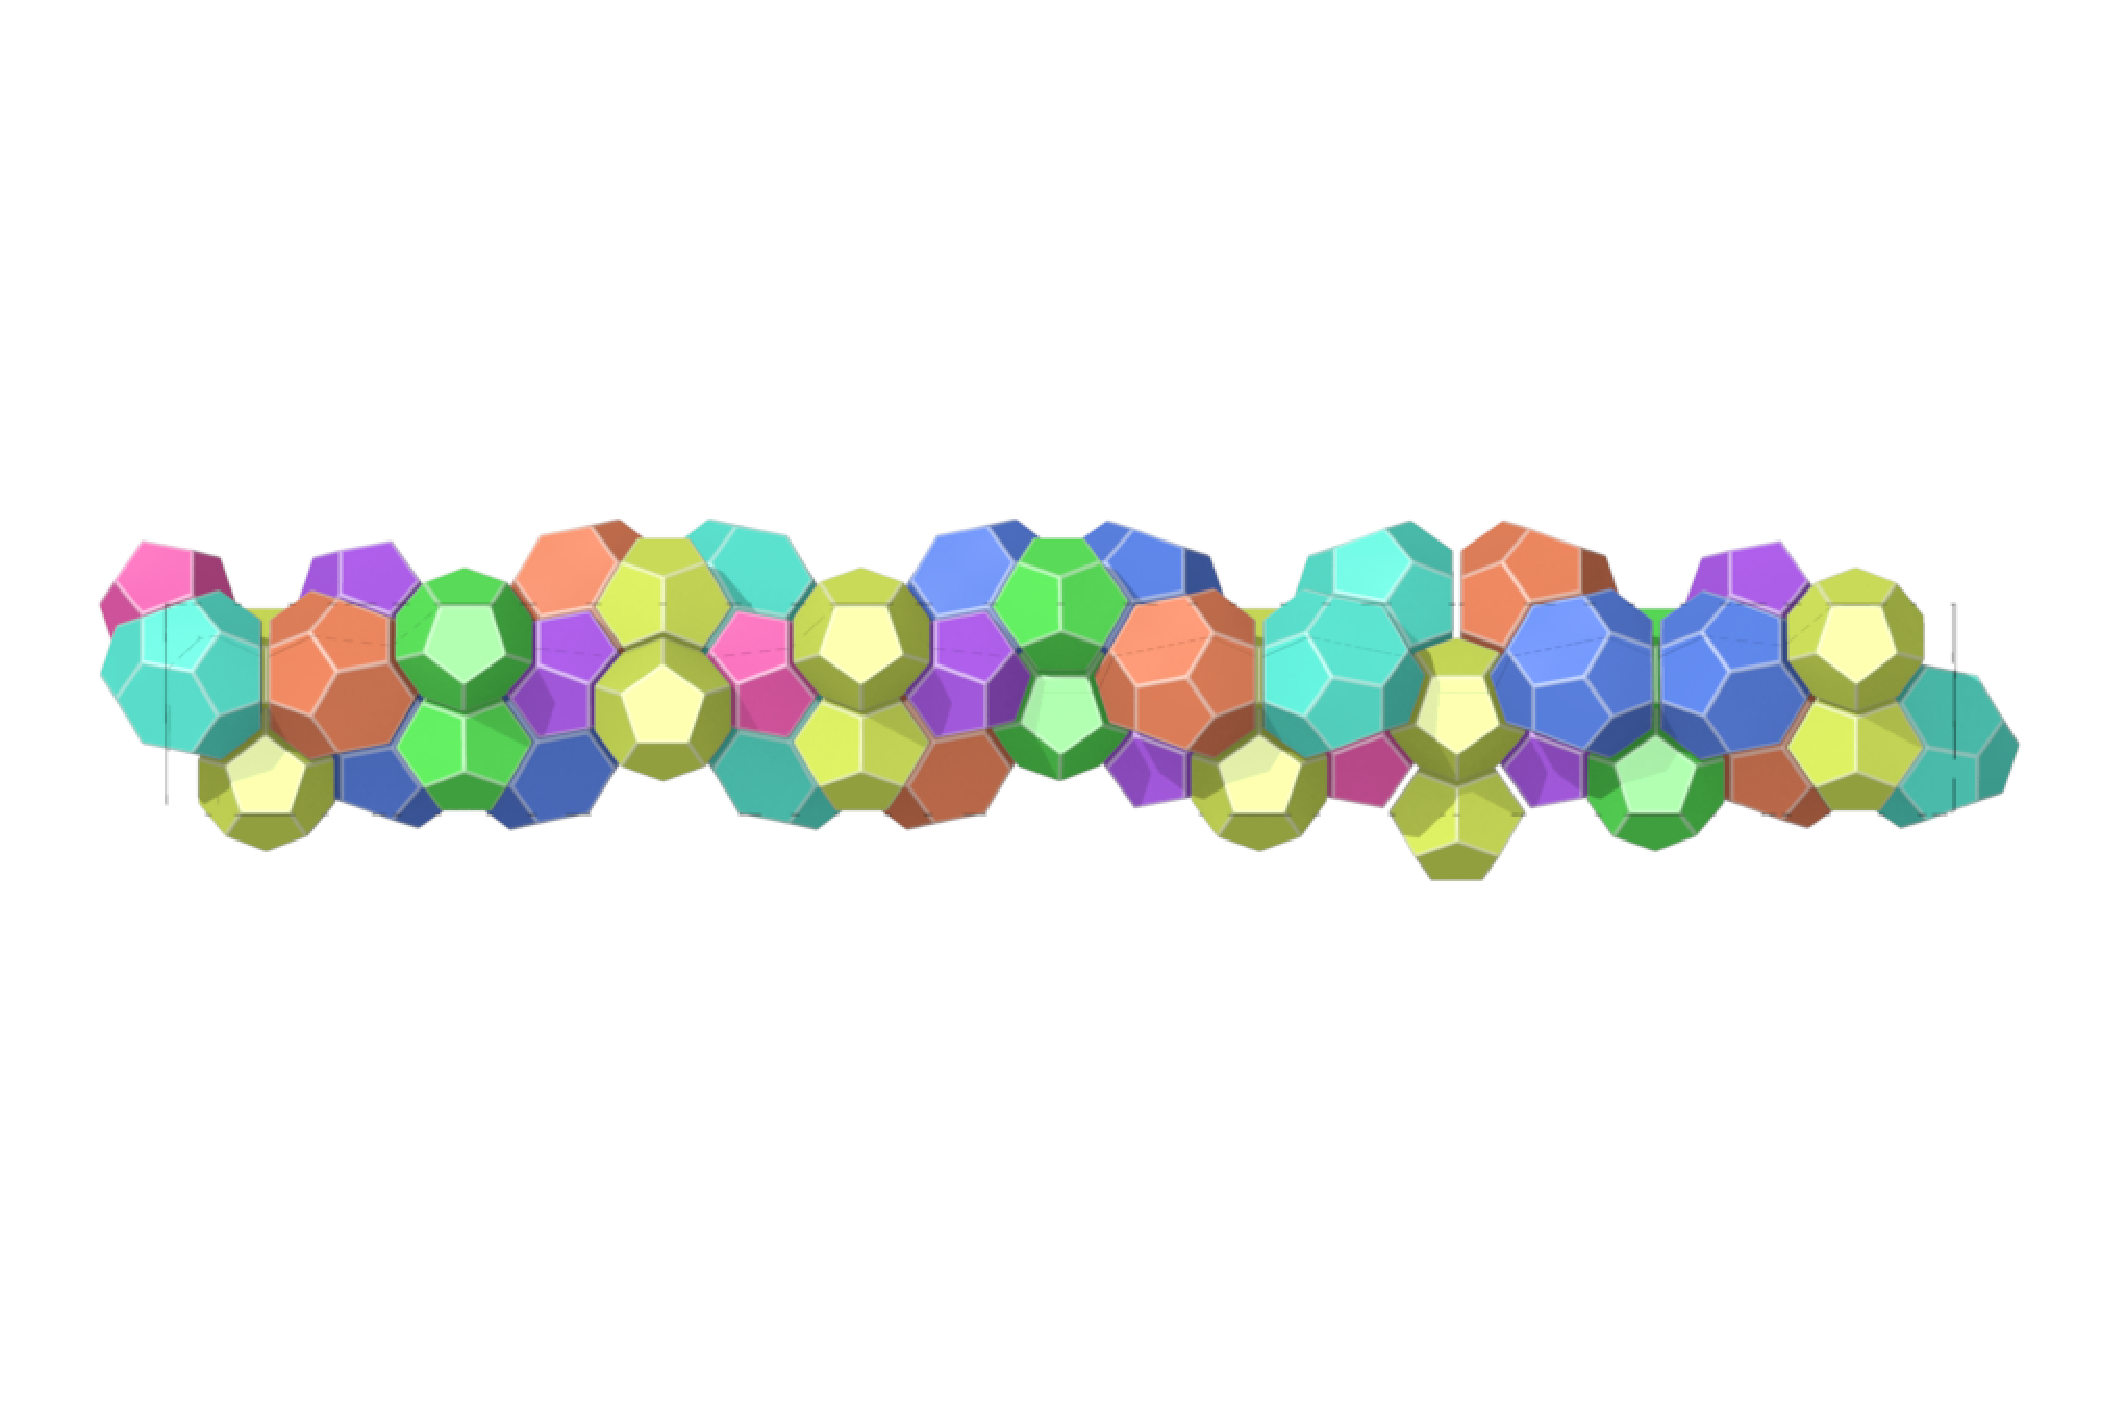
\includegraphics[bb=46 250 970 426, clip]{SpaceFullPicture/PIC20_84_V2/30_25.pdf}}\par
$R\overline{3}m$, $54$
\end{minipage}
\end{center}

}

\frame{
  \frametitle{Some other structures}

\begin{itemize}
\item Also in some mixed clathrate ``ice-like'' hydrates: 
\begin{center}
\begin{tabular}{|c|c|c|c|c|c|c|}
\hline
t.c.p.   & alloys  & exp. clathrate  &\# $20$&\# $24$&\# $26$&\# $28$\\
\hline
$A_{15}$ &$Cr_{3}Si$     & I:$4Cl_2.7H_2O$       &1  &3 &0 &0\\
$C_{15}$ &$MgCu_2$       & II:$CHCl_3.17H_2O$    &2  &0 &0 &1\\
$Z$      &$Zr_4Al_3$     & III:$Br_2.86H_2O$     &3  &2 &2 &0\\
\hline
\end{tabular}
\end{center}
vertices are $H_2O$, hydrogen bonds, cells are sites of solutes ($Cl$, $Br$, \dots).
\item At the olympic games:
\end{itemize}

\begin{center}
\begin{minipage}[b]{4.1cm}
\centering
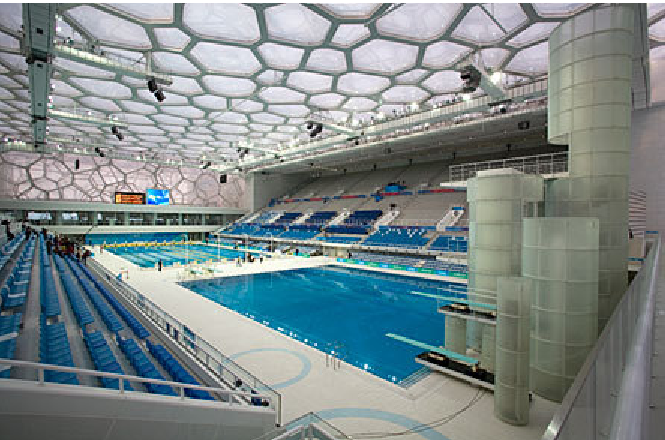
\epsfig{width=3.8cm, file=SpaceFullPicture/SWIMMING_IN_BUBBLES-crop.pdf}\par
%\resizebox{3.8cm}{!}{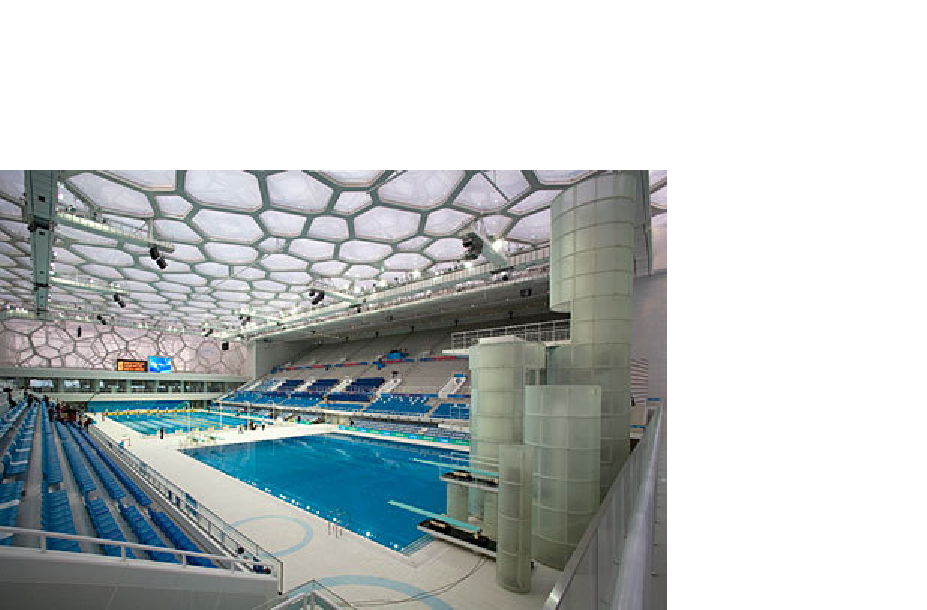
\includegraphics[bb=1 1 320 212, clip]{SpaceFullPicture/SWIMMING_IN_BUBBLES.pdf}}\par
\end{minipage}
\begin{minipage}[b]{4.1cm}
\centering
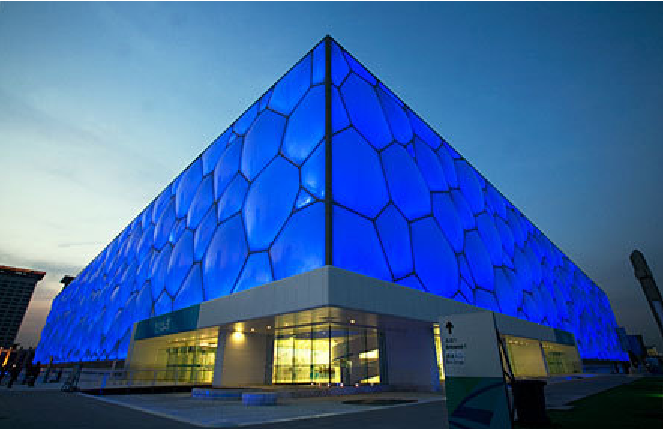
\epsfig{width=3.8cm, file=SpaceFullPicture/WATER_CUBE-crop.pdf}\par
%\resizebox{3.8cm}{!}{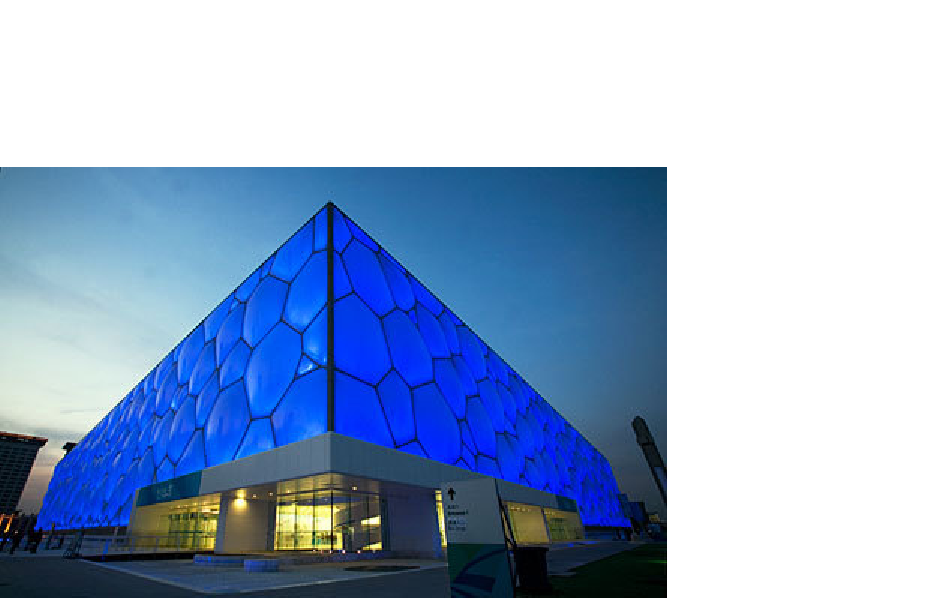
\includegraphics[bb=1 1 319 207, clip]{SpaceFullPicture/WATER_CUBE.pdf}}\par
\end{minipage}
\end{center}
}





\frame{
  \frametitle{Kelvin problem I}
\begin{itemize}
\item The \textcolor{red}{general Kelvin problem} is to partition the Euclidean space $E^n$ by some cells of equal volume and to minimize the surface between cells.
\item In dimension $2$ the solution is known to be the hexagonal structure:
\begin{center}
\begin{minipage}{5.6cm}
\centering
\resizebox{42mm}{!}{\rotatebox{90}{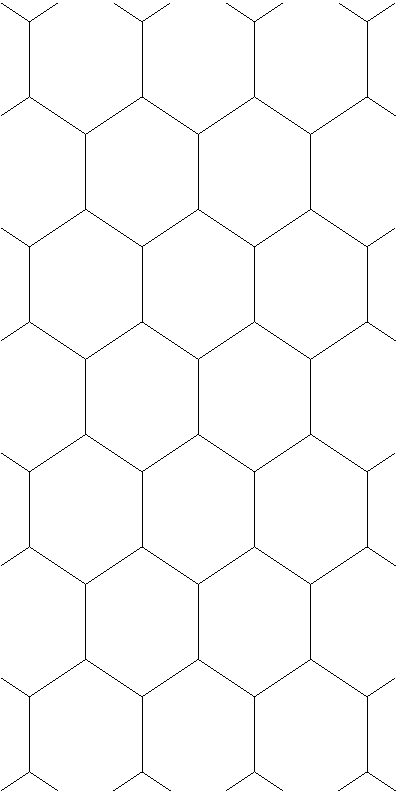
\includegraphics{FigureWythoff/Reg2.pdf}}}\par
\end{minipage}
\end{center}
\begin{itemize}
\item T. Hales, {\em The honeycomb conjecture}. Discrete Comput. Geom. {\bf 25} (2001) 1--22.
\end{itemize}
\item The solution in dimension $3$ is not known but Kelvin proposed a structure, which was the example to beat.
\item F. Almgren proposed to try to beat it by doing variational optimization over periodic structures 
\end{itemize}
}

\frame{
  \frametitle{Kelvin problem II}
\begin{center}
\begin{minipage}[b]{5.0cm}
\centering
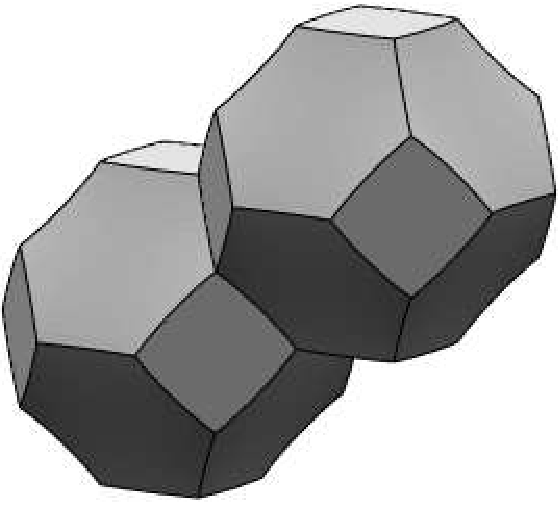
\epsfig{width=4.0cm, file=FullPresPic/kelvinend_4-crop.pdf}\par
%\resizebox{4.0cm}{!}{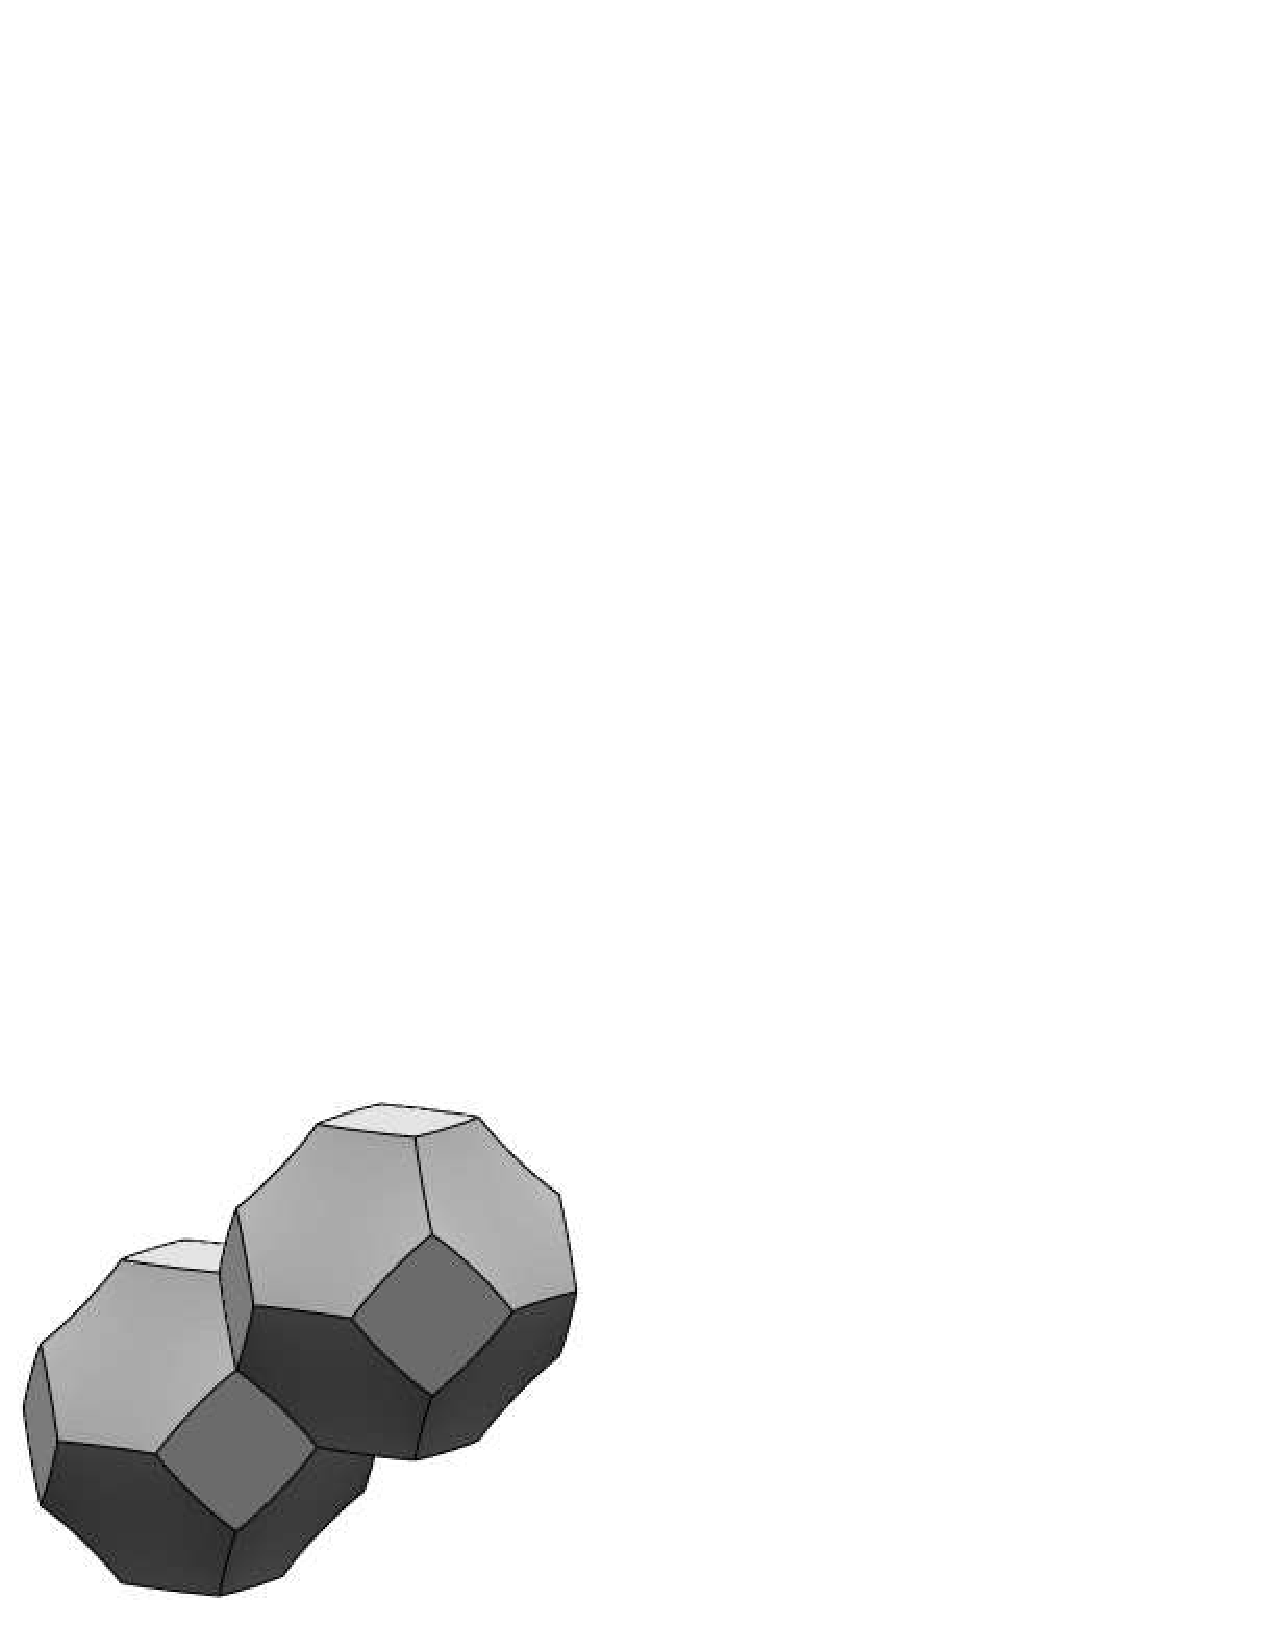
\includegraphics[bb=10 22 278 265, clip]{FullPresPic/kelvinend_4.pdf}}\par
Kelvin's partition
\end{minipage}
\begin{minipage}[b]{5.0cm}
\centering
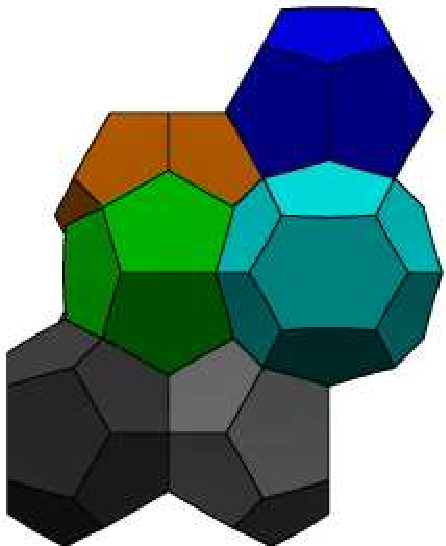
\epsfig{width=3.5cm, file=FullPresPic/wpC_4-crop.pdf}\par
%\resizebox{3.5cm}{!}{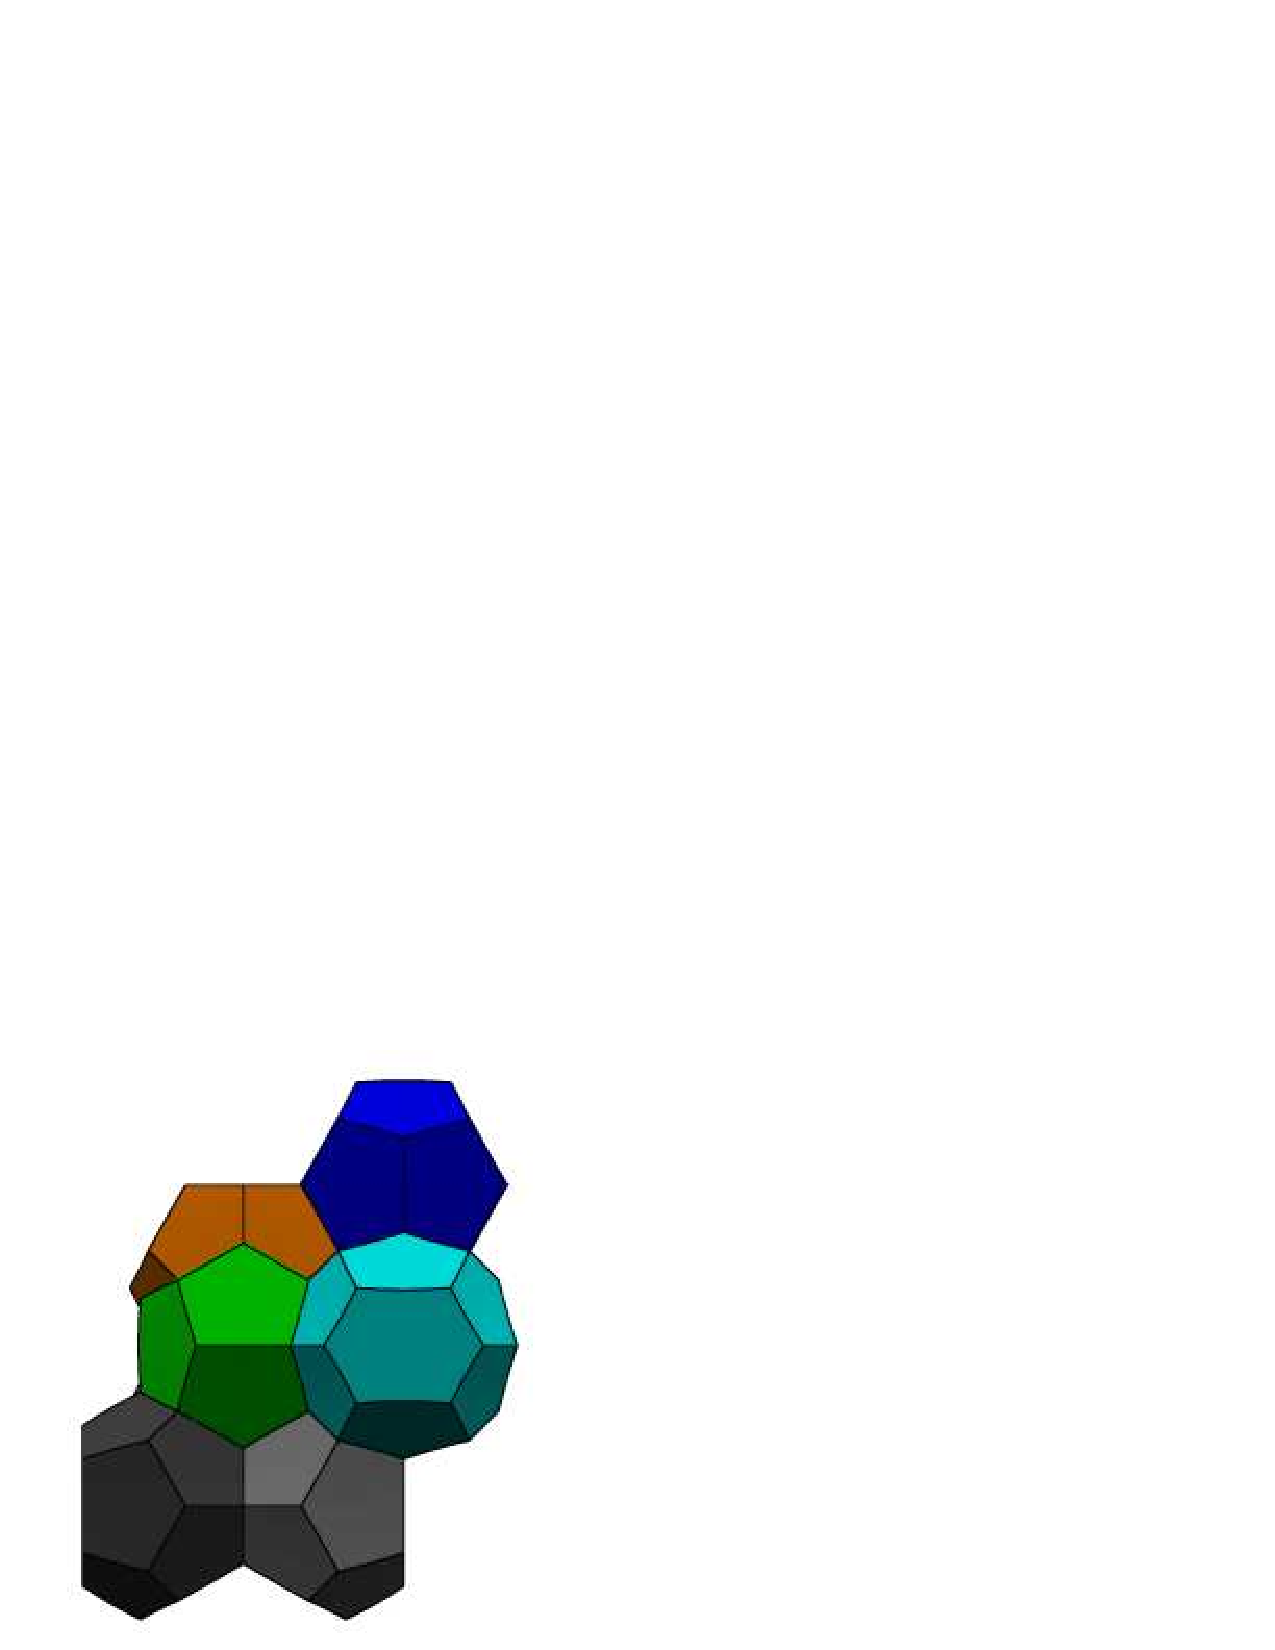
\includegraphics[bb=36 15 250 277, clip]{FullPresPic/wpC_4.pdf}}\par
Weaire, Phelan's partition
\end{minipage}
\end{center}

\begin{itemize}
\item Weaire-Phelan partition ($A_{15}$) is 0.3\% better than Kelvin's (Voronoi polytope of $\mathsf{A}_3^*$)
\item Best is unknown 
\end{itemize}
}





\frame{
\begin{center}
\begin{tabular*}{7cm}{c}
\\[-0.5cm]
{\Huge \textcolor{blue}{II. }\textcolor{red}{Combinatorial}}\\
{\Huge \textcolor{red}{encoding and}}\\
{\Huge \textcolor{red}{topological recognition}}\\
{\Huge \textcolor{red}{problem}}
\end{tabular*}
\end{center}
}


\frame{
  \frametitle{Flags and flag operators}

\begin{itemize}
\item A \textcolor{red}{cell complex} ${\cal C}$ is a family of cells with inclusion relations such that the intersection of any two cells is either empty or a single cell.\\
We also assume it to be pure of dimension $d$, i.e. all inclusion maximal cell have dimension $d$.
\item It is \textcolor{red}{closed} (or has \textcolor{red}{no boundary})
if any $d-1$ dimensional cell is contained in two $d$-dimensional cells.
\item A \textcolor{red}{flag} is an increasing sequence $F_{n_0}\subset F_{n_1}\subset \dots \subset F_{n_r}$ of cells of dimension $n_0,\dots, n_r$. $(n_0,\dots, n_r)$ is the type of the flag.
\item A flag is \textcolor{red}{complete} if its type is $(0,\dots, d)$.
\item Denote by ${\cal F}({\cal C})$ the set of complete flags of ${\cal C}$.
\item If $f=(F_0,\dots, F_d)$ is a complete flag and $0\leq i\leq d$ then the flag $\sigma_i(f)$ is the one differing from $f$ only in the dimension $i$.
\item A cell complex ${\cal C}$ is completely described by the action of $\sigma_i$ on ${\cal F}({\cal C})$.
\item The problem is that ${\cal F}({\cal C})$ may well be infinite or very large to be workable with.
\end{itemize}
}


\frame{
  \frametitle{Illustration with the cube}
\begin{itemize}
\item A flag and its images
\begin{center}
\begin{minipage}[b]{4.0cm}
\centering
\resizebox{2.7cm}{!}{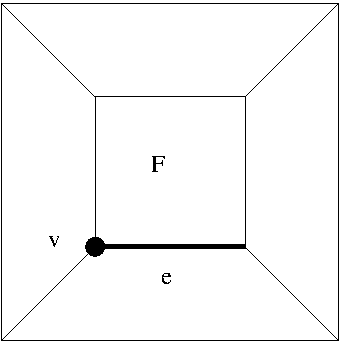
\includegraphics{SpaceFullPicture/CubeFlag.pdf}}\par
Flag $f$
\end{minipage}
\begin{minipage}[b]{4.0cm}
\centering
\resizebox{2.7cm}{!}{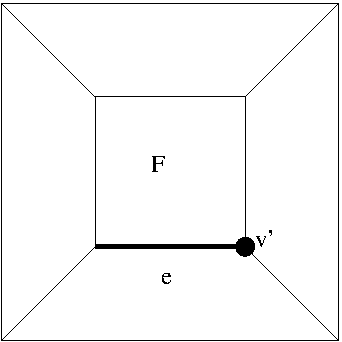
\includegraphics{SpaceFullPicture/CubeFlag_sigma0.pdf}}\par
Flag $\sigma_0(f)$
\end{minipage}
\begin{minipage}[b]{4.0cm}
\centering
\resizebox{2,7cm}{!}{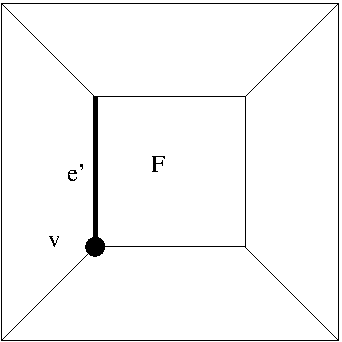
\includegraphics{SpaceFullPicture/CubeFlag_sigma1.pdf}}\par
Flag $\sigma_1(f)$
\end{minipage}
\begin{minipage}[b]{4.0cm}
\centering
\resizebox{2.7cm}{!}{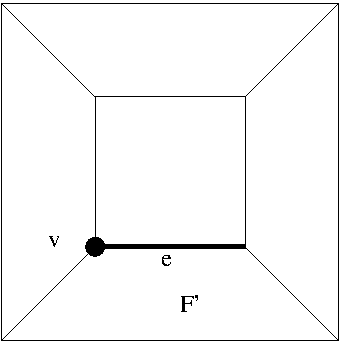
\includegraphics{SpaceFullPicture/CubeFlag_sigma2.pdf}}\par
Flag $\sigma_2(f)$
\end{minipage}
\end{center}
\item The vertices, edges and faces correspond to orbits of $\left\langle\sigma_1, \sigma_2\right\rangle$, 
$\left\langle\sigma_0, \sigma_2\right\rangle$ and $\left\langle\sigma_0, \sigma_1\right\rangle$.




\end{itemize}
}



\frame{
  \frametitle{Delaney symbol}

\begin{itemize}
\item Suppose ${\cal C}$ is a cell complex, with a group $G$ acting on it. The \textcolor{red}{Delaney symbol} of ${\cal C}$ with respect to $G$ is a combinatorial object containing:
\begin{itemize}
\item The orbits $O_k$ of complete flags under $G$
\item The action of $\sigma_i$ on those orbits for $0\leq i\leq d$.
\item For every orbit $O_k$, take $f\in O_k$, the smallest $m$ such that $(\sigma_i\sigma_j)^m(f)=f$ is independent of $f$ and denoted $m_{i,j}(k)$.
\end{itemize}
${\cal C}$ quotiented by $G$ is an \textcolor{red}{orbifold}.
\item If $G=\Aut({\cal C})$ we speak simply of \textcolor{red}{Delaney symbol} of ${\cal C}$
\item \textcolor{blue}{Theorem}: If ${\cal C}$ is a simply connected manifold, then it is entirely described by its Delaney symbol.
\begin{itemize}
\item A.W.M. Dress, {\em Presentations of discrete groups, acting on simply connected manifolds, in terms of parametrized systems of Coxeter matrices---a systematic approach}, Advances in Mathematics {\bf 63-2} (1987) 196--212.
\end{itemize}
\item This is actually a reminiscence of Poincar\'e polyhedron theorem.
\end{itemize}
}


\frame{
  \frametitle{The inverse recognition problem}

\begin{itemize}
\item Suppose we have a Delaney symbol ${\cal D}$, i.e. the data of permutations $(\sigma_i)_{0\leq i\leq d}$ and the matrices $m_{ij}(k)$.
\begin{center}
\begin{tabular}{p{8cm}}
We want to know what is the universal cover manifold ${\cal C}$ (and if it is Euclidean space).
\end{tabular}
\end{center}
\item Some cases:
\begin{itemize}
\item If we have only \textcolor{red}{$1$ orbit of flag} then the Delaney symbol is simply a Coxeter Dynkin diagram and the decision problem is related to the eigenvalues of the Coxeter matrix.
\item If \textcolor{red}{$d=2$} then we can associate a curvature $c({\cal D})$ to the Delaney symbol and the sign determines whether ${\cal C}$ is a sphere, euclidean plane or hyperbolic plane.
\item If \textcolor{red}{$d=3$} then the problem is related to hard questions in $3$-dimensional topology. But the software {\tt Gavrog}/{\tt 3dt} by O. Delgado Friedrichs can actually decide those questions.
\end{itemize}

\end{itemize}
}


\frame{
  \frametitle{Functionalities of {\tt Gavrog}/{\tt 3dt}}


\begin{itemize}
\item It can
\begin{itemize}
\item Test for euclidicity of Delaney symbols, that is recognize when ${\cal C}$ is Euclidean space.
\item Find the minimal Delaney symbol, i.e. the representation with smallest fundamental domain and maximal group of symmetry.
\item Compute the space group of the crystallographic structure.
\item Test for isomorphism amongst minimal Delaney symbols.
\item Create pictures, i.e. metric informations from Delaney symbols.
\end{itemize}
\item All this depends on difficult questions of $3$-dimensional topology, now mostly solved.
This means that in theory the program does not always works, but in practice it does.
\begin{itemize}
\item[\textcolor{red}{\ding{224}}] O. Delgado Friedrichs, {\em 3dt - Systre},
\begin{center}
\url{http://gavrog.sourceforge.net}
\end{center}
\item[\textcolor{red}{\ding{224}}] O. Delgado Friedrichs, {\em Euclidicity criteria}, PhD thesis.
\end{itemize}

\end{itemize}
}






\frame{
\begin{center}
\begin{tabular*}{7cm}{c}
\\[-0.5cm]
{\Huge \textcolor{blue}{III. }\textcolor{red}{The combinatorial}}\\
{\Huge \textcolor{red}{enumeration problem}}\\
\end{tabular*}
\end{center}
}






\frame{
  \frametitle{Proposed enumeration method}
\begin{itemize}
\item All periodic tilings can be described combinatorially by Delaney symbol.
\begin{itemize}
\item But is it good for enumeration? No, because the number of flags may be too large.
\item So, we choose not to use it for the generation of the tilings.
\end{itemize}
\item We are enumerating closed orientable $3$-dimensional manifolds with $N$ maximal cells, i.e. with an additional requirement:
\begin{itemize}
\item Every maximal cell $C$ is adjacent only to maximal cells $C'$ with $C'\not= C$.
\end{itemize}
The crystallographic structure is obtained as universal cover.
\item A partial tiling is an agglomeration of tiles, possibly with some holes.
\item The method is thus to add tiles in all possibilities and to consider adding tiles in all possible ways.
\end{itemize}
}



\frame{
  \frametitle{Tree search}
\begin{itemize}
\item When we are computing all possibilities, we are adding possible tiles one by one. All options are considered sequentially.
\item This means that we need to store in memory only the previous choices, i.e. if a structure is made of $N$ maximal cells $C_1, \dots, C_N$, then we simply have to store:
\begin{equation*}
\begin{array}{c}
\{C_1\}\\
\{C_1, C_2\}\\
\{C_1, C_2,C_3\}\\
\vdots\\
\{C_1, C_2,\dots, C_N\}\\
\end{array}
\end{equation*}
This is memory efficient.
\item There are two basic movement in the tree: go deeper or go to the next choice (at the same or lower depth).
%\item With \textcolor{red}{Orderly Enumeration} it is possible to use symmetries to go faster in the tree search.
\end{itemize}
}

\frame{
  \frametitle{Computer Science \& Orderly enumeration}
\begin{itemize}
\item The tree search needs very little memory, if $N$ cells are put, we need to store only $N+1$ levels.
\item It is entirely processors limited, with the program going over all possibilities.
\item Since it is a tree search, we can parallelize very easily: Each process runs its own part of the tree.
\item The problem is that a same structure can be obtained in many equivalent ways.
\item With \textcolor{red}{orderly enumeration} one can enumerate lexicographically minimal representations among all equivalent representations
\item See for more details
\begin{itemize}
\item M. Dutour Sikiri\'c, O. Delgado-Friedrichs, M. Deza, Space fullerenes: computer search for new Frank-Kasper structures, Acta crystallographica A {\bf 66} (2010) 602--615
\item M. Dutour Sikirić, M. Deza, Space fullerenes: computer search for new Frank-Kasper structures II, Structural Chemistry {\bf 23-4} (2012) 1103--1114
\end{itemize}
\end{itemize}
}






\frame{
\begin{center}
\begin{tabular*}{7cm}{c}
\\[-0.5cm]
{\Huge \textcolor{blue}{IV. }\textcolor{red}{The obtained}}\\
{\Huge \textcolor{red}{structures}}
\end{tabular*}
\end{center}
}




\frame{
  \frametitle{Enumeration results}
\begin{itemize}
\item We enumerate periodic structures having a fundamental domain containing at most $N$ maximal cells.
\item Note that the cells are not all congruent, Dodecahedron is not necessarily regular and the faces of ``polytopes'' can be curved.
\item For every structure, we have a fractional formula $(x_{20}, x_{24}, x_{26}, x_{28})$.
\item For $N=20$, we get $84$ structures in $1$ month of computations on about $200$ processors.
Going from $N$ to $N+1$, computation time multiply by around $2.3$.
\end{itemize}

{\scriptsize
\begin{center}
\begin{tabular}{||c|c||c|c||c|c||}
\hline
$(1,3,0,0)$ & $1$ & $(2,0,0,1)$ & $5$ & $(3,2,2,0)$ & $4$\\
$(3,3,0,1)$ & $3$ & $(3,3,2,0)$ & $1$ & $(3,4,2,0)$ & $3$\\
$(4,5,2,0)$ & $1$ & $(5,2,2,1)$ & $20$ & $(5,3,0,2)$ & $3$\\
$(5,8,2,0)$ & $2$ & $(6,5,2,1)$ & $6$ & $(6,11,2,0)$ & $1$\\
$(7,2,2,2)$ & $5$ & $(7,4,2,2)$ & $1$ & $(7,7,4,0)$ & $1$\\
$(7,8,2,1)$ & $1$ & $(8,4,4,1)$ & $2$ & $(8,5,2,2)$ & $2$\\
$(9,2,2,3)$ & $1$ & $(10,3,6,1)$ & $3$ & $(10,5,2,3)$ & $6$\\
$(11,1,4,3)$ & $1$ & $(11,2,2,4)$ & $11$ & &\\
\hline
\end{tabular}
\end{center}
}
}


\frame{
  \frametitle{The $A_{15}$ structure $(1,3,0,0)$}

\begin{center}
\resizebox{9.5cm}{!}{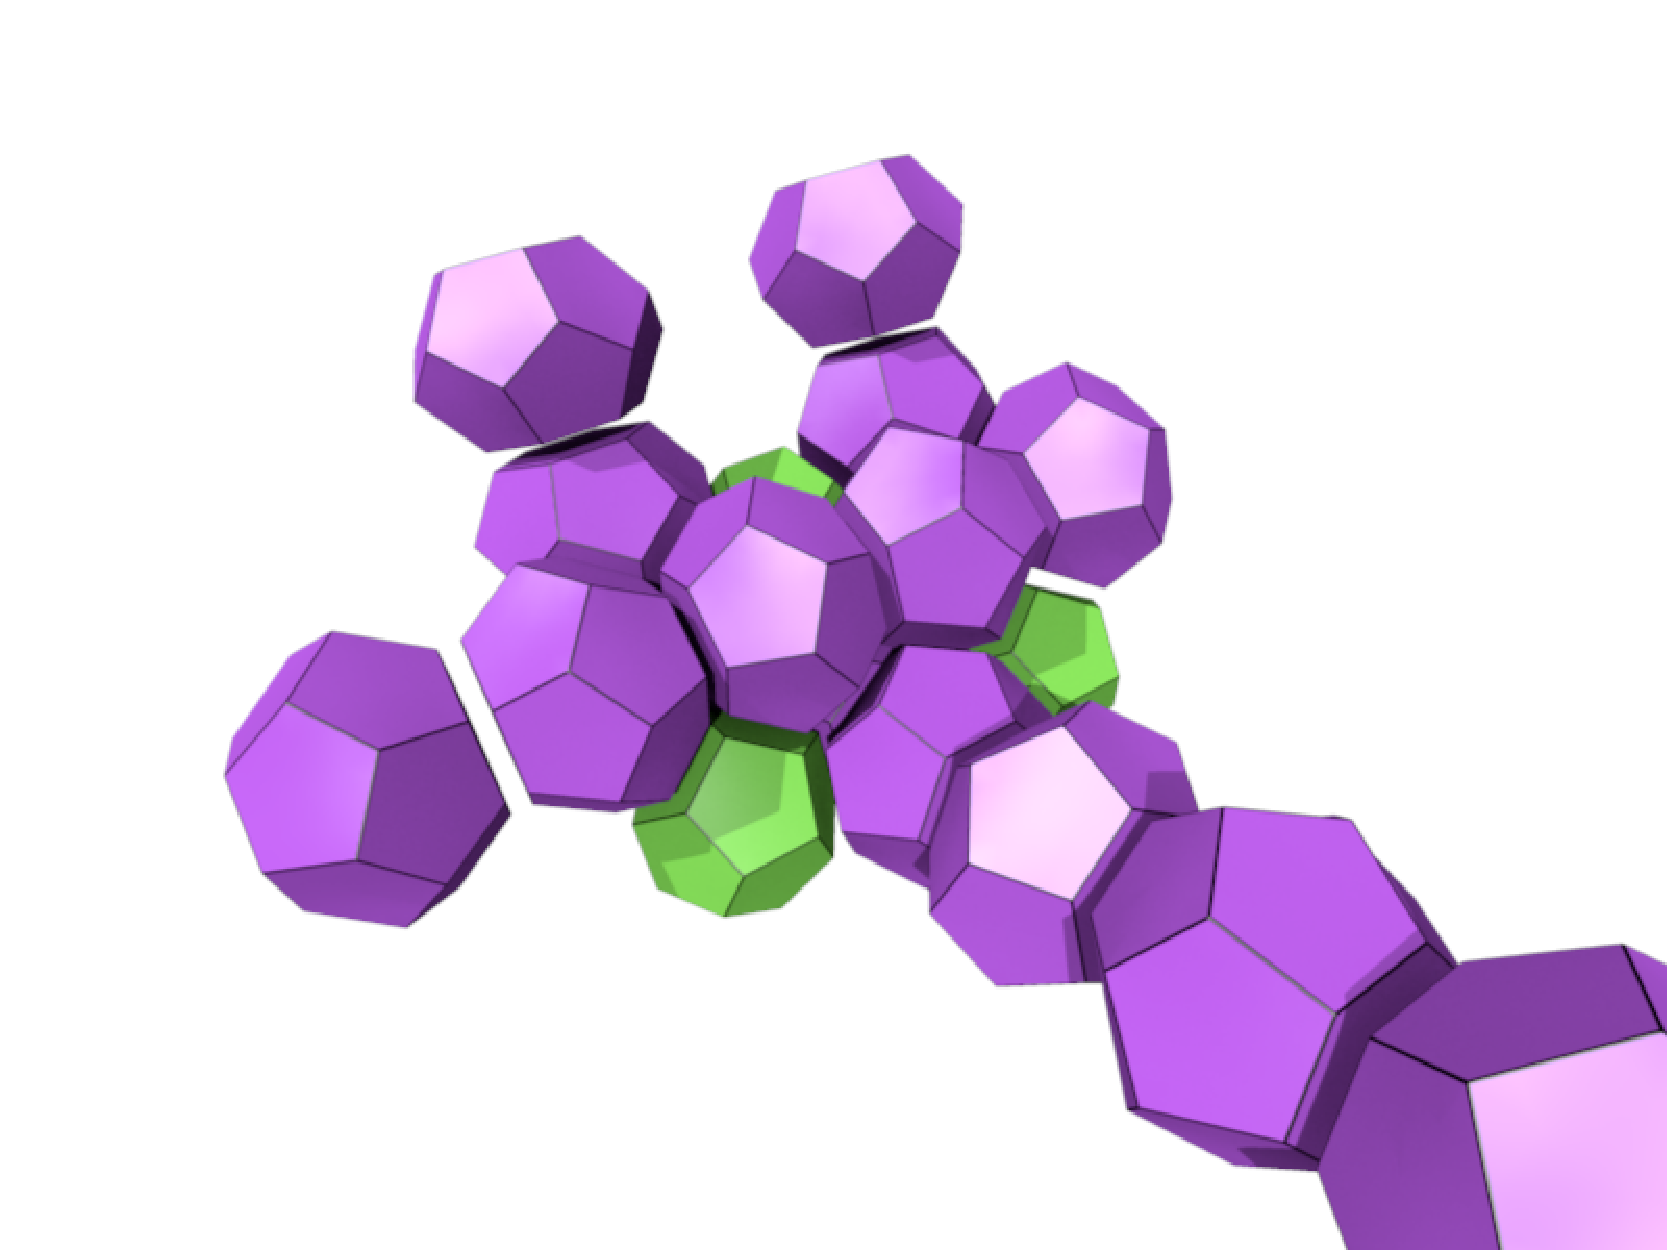
\includegraphics{SpaceFullPicture/A15_1bis.pdf}}\par
\end{center}
Uniquely determined by fractional composition.
}
\frame{
  \frametitle{The $Z$ structure $(3,2,2,0)$}

\begin{center}
\resizebox{9.5cm}{!}{\includegraphics{SpaceFullPicture/Struct7.pdf}}\par
\end{center}
}
\frame{
  \frametitle{One Laves structure $(2,0,0,1)$}

\begin{center}
\resizebox{9.5cm}{!}{\includegraphics{SpaceFullPicture/Struct1.pdf}}\par
\end{center}
The $28$ maximal cells forms a diamond structure named $C_{15}$.
The most basic Laves structure.
}






\frame{
  \frametitle{Other structure $(3,2,2,0)$}

\begin{center}
\resizebox{9.5cm}{!}{\includegraphics{SpaceFullPicture/Struct14_63.pdf}}\par
\end{center}
}
\frame{
  \frametitle{Other structure $(3,2,2,0)$}

\begin{center}
\resizebox{9.5cm}{!}{\includegraphics{SpaceFullPicture/Struct14_65.pdf}}\par
\end{center}
}
\frame{
  \frametitle{Other structure $(3,2,2,0)$}

\begin{center}
\resizebox{9.5cm}{!}{\includegraphics{SpaceFullPicture/Struct14_78.pdf}}\par
\end{center}
}







\frame{
  \frametitle{One structure $(3,3,0,1)$}

\begin{center}
\resizebox{9.5cm}{!}{\includegraphics{SpaceFullPicture/Struct14_52.pdf}}\par
\end{center}
}
\frame{
  \frametitle{One structure $(3,3,0,1)$}
\begin{center}
\resizebox{9.5cm}{!}{\includegraphics{SpaceFullPicture/Struct14_54.pdf}}\par
\end{center}
}
\frame{
  \frametitle{One structure $(3,3,0,1)$}

\begin{center}
\resizebox{9.5cm}{!}{\includegraphics{SpaceFullPicture/Struct14_74.pdf}}\par
\end{center}
}








\frame{
  \frametitle{One structure $(7,2,2,2)$}

\begin{center}
\resizebox{9.5cm}{!}{\includegraphics{SpaceFullPicture/Struct39.pdf}}\par
\end{center}
It is a mix of $C_{15}$ and $A_{15}$ in layers.
}



\frame{
  \frametitle{One structure $(7,2,2,2)$}

\begin{center}
\resizebox{9.5cm}{!}{\includegraphics{SpaceFullPicture/Struct41.pdf}}\par
\end{center}
It is a mix of $Z$ and $C_{15}$ in layers.
}

\frame{
  \frametitle{One structure $(5,2,2,1)$}

\begin{center}
\resizebox{9.5cm}{!}{\includegraphics{SpaceFullPicture/Struct18.pdf}}\par
\end{center}
%It is a mix of $Z$ and $C_{15}$ in layers.
}





\frame{
  \frametitle{One structure $(4,5,2,0)$}

\begin{center}
\resizebox{9.5cm}{!}{\includegraphics{SpaceFullPicture/Struct19.pdf}}\par
\end{center}
It is a mix of $Z$ and $A_{15}$ in layers.
}









\frame{
\begin{center}
\begin{tabular*}{7cm}{c}
\\[-0.5cm]
{\Huge \textcolor{blue}{V. }\textcolor{red}{Special}}\\
{\Huge \textcolor{red}{constructions}}\\
\end{tabular*}
\end{center}
}





\frame{
  \frametitle{Tiling by buckminsterfullerene}

\begin{itemize}
\item Does there exist space-fullerenes with maximal cells being soccer balls (i.e. buckminsterfullerenes)?
\item Given a type $T$ of flag and a closed cell complex ${\cal C}$ it is possible to build a cell complex ${\cal C}(T)$, named \textcolor{red}{Wythoff construction}, \textcolor{red}{Shadow geometry}, \textcolor{red}{Grassmann geometry}, \textcolor{red}{Kaleidoscope construction}, etc.
\item Examples:
\begin{itemize}
\item If $T=\{0\}$, then ${\cal C}(T)={\cal C}$ (identity)
\item If $T=\{d\}$, then ${\cal C}(T)={\cal C}^{*}$ (i.e. the dualof ${\cal C}$)
\item If $T=\{0,\dots, d\}$, then ${\cal C}(T)$ is the order complex.
\end{itemize}
\item The answer is that such space fullerenes are obtained by applying $T=\{0,1\}$ to the Coxeter geometry of diagram $(5,3,5)$, which is hyperbolic. So, no such object exist as a polytope or as a space-fullerene
\begin{itemize}
\item A. Pasini, {\em Four-dimensional football, fullerenes and diagram geometry}, Discrete Math {\bf 238} (2001) 115--130.
\end{itemize}

\end{itemize}
}



\frame{
  \frametitle{A special tiling by fullerenes}

\textcolor{red}{Deza and Shtogrin}: There exist tilings by fullerenes
different from $F_{20}$, $F_{24}$, $F_{26}$ and $F_{28}(T_d)$.
By $F_{20}$, $F_{24}$ and its elongation $F_{36}(D_{6h})$
in ratio $7:2:1$;

\begin{center}
\begin{minipage}[b]{5.0cm}
\centering
\epsfig{width=4.1cm, file=FullPresPic/Scrn1s-crop.pdf}\par
%\resizebox{4.1cm}{!}{\includegraphics[bb=1 4 434 485, clip]{FullPresPic/Scrn1s.pdf}}\par
\end{minipage}
\begin{minipage}[b]{5.0cm}
\centering
\epsfig{width=4.1cm, file=FullPresPic/Scrn3s-crop.pdf}\par
%\resizebox{4.1cm}{!}{\includegraphics[bb=3 3 511 595, clip]{FullPresPic/Scrn3s.pdf}}\par
\end{minipage}
\end{center}
\begin{itemize}
\item \textcolor{red}{Delgado Friedrichs, O'Keeffe}: All tiling by fullerenes with at most $7$ kinds of flags: $A_{15}$, $C_{15}$, $Z$, $\sigma$ and this one.
\end{itemize}
}





\frame{
  \frametitle{Yarmolyuk Kripyakevich conjecture}

\begin{itemize}
\item They conjectured that for a space fullerene to exist, we should have 
\begin{equation*}
-x_{20}+\frac{x_{24}}{3}+\frac{7}{6}x_{26}+2x_{28} = 0
\end{equation*}
\item But some counterexamples were found:
\begin{center}
\epsfig{width=7.5cm, file=SpaceFullPicture/Struct14_17-crop.pdf}\par
%\resizebox{7.5cm}{!}{\includegraphics[bb=20 47 752 498, clip]{SpaceFullPicture/Struct14_17.pdf}}\par
\end{center}
\item Some other conjecture are broken.

\end{itemize}
}


%\frame{
%  \frametitle{Other counterexample}
%
%\begin{itemize}
%\item 
%\end{itemize}
%}





\frame{
  \frametitle{The Sadoc-Mosseri inflation I}

\begin{itemize}
\item Call ${\rm snub Prism}_5$ the Dodecahedron and ${\rm snub Prism}_6$ the fullerene $F_{24}$.
\item Given a space fullerene ${\cal T}$ by cells $P$, we define the inflation $IFM({\cal T})$ to be the simple tiling such that
\begin{itemize}
\item Every cell $P$ contains a shrunken copy $P'$ of $P$ in its interior.
\item On every vertices of $P$ a $F_{28}$ has been put.
\item On every face of $P'$ with $m$ edges, a $snub\,Prism_{m}$ is put
which is contained in $P$.
\end{itemize}
\item Thus for individual cells $F_{20}$, $F_{24}$, $F_{26}$, $F_{28}$ the operations goes as follows:
\begin{equation*}
\left\{\begin{array}{rcl}
F_{20} &\rightarrow & F_{20} + 12 F_{20} + \frac{20}{4} F_{28}\\
F_{24} &\rightarrow & F_{24} + \{12 F_{20} + 2F_{24}\} + \frac{24}{4} F_{28}\\
F_{26} &\rightarrow & F_{26} + \{12 F_{20} + 3F_{24}\} + \frac{26}{4} F_{28}\\
F_{28} &\rightarrow & F_{28} + \{12 F_{20} + 4F_{24}\} + \frac{28}{4} F_{28}
\end{array}\right.
\end{equation*}

\end{itemize}
}




\frame{
  \frametitle{The Sadoc-Mosseri inflation II}

\begin{itemize}
\item The inflation on the $A_{15}$ structure: the shrunken cells of $A_{15}$ and the generated $F_{28}$
\end{itemize}

\begin{center}
\begin{minipage}[b]{4.1cm}
\centering
\epsfig{width=3.8cm, file=SpaceFullPicture/IFM_A15_1-crop.pdf}\par
%\resizebox{3.8cm}{!}{\includegraphics[bb=202 34 815 644, clip]{SpaceFullPicture/IFM_A15_1.pdf}}\par
\end{minipage}
\begin{minipage}[b]{4.1cm}
\centering
\epsfig{width=3.8cm, file=SpaceFullPicture/IFM_A15_2-crop.pdf}\par
%\resizebox{3.8cm}{!}{\includegraphics[bb=203 33 815 644, clip]{SpaceFullPicture/IFM_A15_2.pdf}}\par
\end{minipage}
\end{center}
}





\frame{
  \frametitle{The Frank Kasper Sullivan construction I}

\begin{itemize}
\item The construction is first described in Frank \& Kasper, 1959 but a better reference is:
\begin{itemize}
\item J.M. Sullivan, {\em New tetrahedrally closed-packed structures}.
\end{itemize}
\item We take a tiling of the plane by regular triangle and regular squares and define from it a space fullerene with $x_{28}=0$.
\item Every edge of the graph is assigned a color (\textcolor{red}{red} or \textcolor{blue}{blue}) such that
\begin{itemize}
\item Triangles are monochromatic
\item colors alternate around a square.
\end{itemize}
\item Local structure is
\begin{center}
\begin{minipage}[b]{5.0cm}
\centering
\resizebox{4.1cm}{!}{\includegraphics{SpaceFullPicture/LocalSullivanStructure.pdf}}\par
\end{minipage}
\end{center}
\end{itemize}
}

\frame{
  \frametitle{The Frank Kasper Sullivan construction II}

\begin{itemize}
\item The construction explains a number of structures:
\end{itemize}
\begin{center}
\begin{minipage}[b]{10.0cm}
\centering
\resizebox{9.5cm}{!}{\includegraphics{SpaceFullPicture/SullivanCases.pdf}}\par
\end{minipage}
\end{center}
\begin{itemize}
\item Actually a structure with $x_{28}=0$ is physically realized if and only if it is obtained by this construction.
\item Another name is \textcolor{red}{Hexagonal t.c.p.} since there are infinite columns of $F_{24}$ on each vertex of the tesselation by triangle and squares.
\end{itemize}
}


\frame{
  \frametitle{Pentagonal t.c.p. I. general}

\begin{itemize}
\item Those structures are described in
\begin{itemize}
\item Shoemaker C.B. and Shoemaker D., {\em Concerning systems for the generation and coding of layered, tetrahedrally closed-packed structures of intermetallic compounds}, Acta Crystallographica (1972) \textbf{B28} 2957--2965.
\end{itemize}
They generalize Laves phases, generalized Laves phases (by Frank and Kasper) and various constructions by Pearson Shoemaker and Kripyakevich.
\item The input of the construction is a plane tiling by, not necessarily regular, quadrangles and triangles
with vertex configuration $(3^6)$, $(3^3, 4^2)$,
$(4^4)$, $(3^5)$, $(3^4, 4)$ and $(3^5,4)$ being allowed.
Some of the edges are doubled and the non-doubled edges are colored
in red and blue so that:
\begin{itemize}
\item Every square contains exactly two doubled edges on opposite sides.
\item Every triangle contains exactly one double edge.
\item For every face the non-doubled edges are of the
same color.
\item If two faces share a black edge then their color (red or blue)
is the same if and only if their size are different.
\end{itemize}
\end{itemize}
}


\frame{
  \frametitle{Pentagonal t.c.p. II. general}
\begin{itemize}
\item The result is a FK space fullerene with $x_{24}=x_{26}$.
\item The structure is organized in layers with alternating structures.
\begin{center}
\begin{minipage}[b]{7.0cm}
\centering
\resizebox{6.1cm}{!}{\includegraphics{SpaceFullPicture/ConfigurationTCP.pdf}}\par
\end{minipage}
\end{center}
\item We have:
\begin{itemize}
\item chains of Dodecahedron on each vertex (hence the name \textcolor{red}{Pentagonal t.c.p.}).
\item Dodecahedron on doubled edges
\item $24$-cells and $26$-cells inside squres.
\item $28$-cells near the triangles.
\end{itemize}

\end{itemize}
}


\frame{
  \frametitle{Pentagonal t.c.p. III. Laves phases}

\begin{center}
\input{SpaceFullPicture/PentagonalShSh_Laves.pdf_t}
\end{center}
}



\frame{
  \frametitle{Pentagonal t.c.p. IV. generalized Laves phases}

\begin{center}
\input{SpaceFullPicture/PentagonalShSh_GenLaves.pdf_t}
\end{center}
}


\frame{
  \frametitle{Pentagonal t.c.p. V. sporadic structures}

\begin{center}
\input{SpaceFullPicture/PentagonalShSh_Sporadic.pdf_t}
\end{center}
}






\end{document}
